\documentclass{article}
\usepackage[utf8]{inputenc}
\usepackage{fullpage} % Package to use full page
\usepackage{parskip} % Package to tweak paragraph skipping
\usepackage{tikz} % Package for drawing
\usepackage{float}
\usepackage{subfig}
\usepackage{amsmath}
\usepackage{hyperref}
 
\title{Benediction Final Report}
\author{Group Members: 1862457 Chayanit Krairit , 1781404 Isaac Muhumuza,\\ 1846353 Jihye Hwang, 1833095 Yao Te-Chien, \\1863752 Yan Li, 1876334 Yiwei Zhang}
\date{28th March 2019}

\begin{document}

\maketitle

\section{Introduction}
This project details the work undertaken to develop a multi-person large system; a file synchroniser system that's secure and enables multiple users on different platforms to upload, download, delete files with conflict resolution and in synchronisation with a single server. Development involved 6 members in a group to undertake certain tasks in a waterfall project management approach. 3 teams were set-up; a mobile, back-end and front-end team to develop the application. A number of languages and platforms were used including Node.js, Swift, React, Express as will be seen later in this report.  
Additionally, a public central repository; GitHub was used to support the project and developmental management as well as code hosting and access, seamless changes, peer review and many more whilst also following feature branch/pull request (PR) development.

The file synchroniser system developed for this project supports a hub and spoke; single central server (hub) hosted on the google cloud platform to which multiple clients (spokes) both mobile (standalone application) and desktop can connect, it also allows for file synchronisation between clients and server in real-time. The application supports explicit file transfer between the server and client, file synchronisation, and uses a locking mechanism to prevent conflicts where two users might try and update the same file simultaneously. Furthermore, security mechanisms for logging in and secure end-points was implemented using JSON web token (JWT) and MD5 hashing for passwords.


\section{Review}
In this project, the system will be developed in a similar idea to Dropbox and Microsoft OneDrive. Similarities between all are the ability to store and access files from anywhere, i.e. a computer, phone or tablets, creating and logging into the user accounts and any file changes are automatically synced to a server. This system will however take files uploaded to the server as being up-to-date, allowing every client to fetch the latest file from the server.

The system is accessible only through logging in and there exists a local folder in the application directory for each user that is automatically synced to the central server. Users can move or copy files from their local hard drive to this folder, make modifications, delete and download and each action will be synced with the server. downloading files from the server into this folder will make sure the user has access to the latest files.

The system's mobile application uses HTTP methods with the help of a Swift library \cite{c11} for performing HTTP requests and follows the traditional TableView design \cite{c19}. The team only uses the POST and GET methods to interact with the server to create/update resources.

\section{Requirements and Design}
\subsection{Requirements}
The aim for this project is to create the ‘hub and spoke’ file synchroniser. A single central server is needed to host the server-side files and back-end API that will interact with client-side UI and synchronise local user files. The hub is required to speak a network protocol to clients, be able to deal with multiple simultaneous clients and handling conflicts. Two separate clients will be developed for this project; a desktop client which can be a command-line or background utility and a mobile client which will be a stand-alone application. Having at least 2 clients will allow files to be uploaded onto the server with different users on different platforms. This will ensure that the server will be able to handle multiple simultaneous clients and clashes of having identical copies of the same files.\newline

To tackle this problem, the team has decided to divide into 3 sub-teams: a mobile client team, a desktop client team and back-end server team to ensure that every member contributes to the system’s implementation and to be able to complete all the tasks required. Each sub-team has created a Gantt chart that acts as a guide to complete this project and was then combined with input from the group as a whole to create a complete planning schedule for the project. The figure below shows the overall Gantt chart for this project.

\begin{figure}[H]
\begin{center}
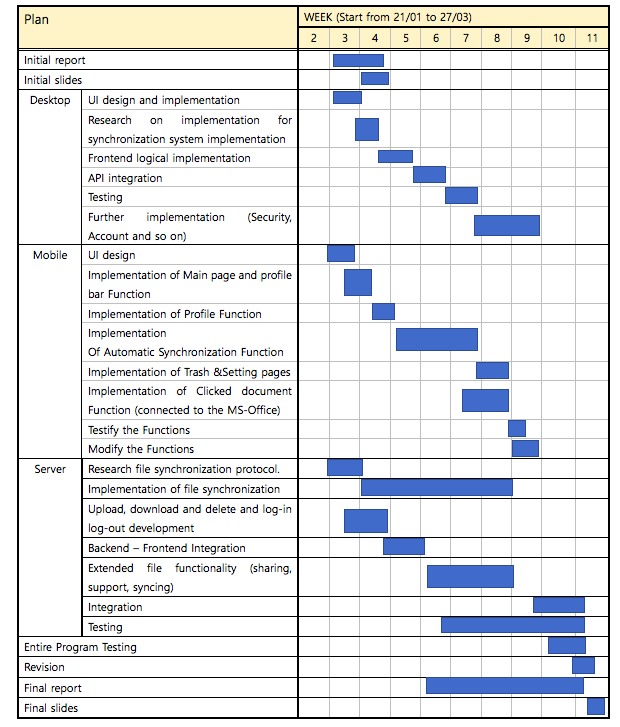
\includegraphics[width=7cm]{timetable.png}
\end{center}
\caption{Benediction Gantt Chart}\label{ex4}
\end{figure}

After group consultation and input, the desktop client team’s work was to develop a react desktop application for users to conveniently use the user interface (UI) to upload, modify and download files from the server instead of using the command-line. 
The mobile client team’s requirement was to implement an application in the iOS environment as the members have previous iOS development experience. The back-end team‘s requirement was to develop a server API to handle clients request and a WebSocket server to sync server-side changes with the client. \newline

The team decided to reconsider the objectives initially proposed in the group's initial report as one of the members suggested a change on the system. The team agreed agreed to a log in and or sign up development for a user to get access to the system. This will help to identify each individual user when they are using the system. Furthermore, the team have also removed the 'extend the support for file types' in the optional objectives as the team believes that the user should be able to upload or download any files they want to/from the server.
The updated objectives for this project is as follows:

\begin{itemize}
  \item Develop a main server, a web and desktop client and a mobile client (based on iOS).
  \item Create Log-in page and users are required to log-in before accessing the files.
  \item Clients must be able to upload, download, modify and delete files.
  \item Local user files must be in sync with the main server files.
  \item Software testing and integration.
\end{itemize}
The optional objectives to be considered as an advanced implementation to the project with time permitting are:
\begin{itemize}
  \item Implement security algorithms to protect private information and address the security system running smoothly.
  \item Apply encryption, decryption, compression and sharing functions to local files.
\end{itemize}

The \emph{Waterfall} model is used as a planning model for this project, where the whole process of this project is divided into separate phases \cite{c3}. The phases of this project are: Requirements, Design, Implementation, Testing and Evaluation. The team will only begin the next phase only after the previous one is complete. The team has decided to use this model as it is easy to understand and helps the team to work towards a goal each time as the schedule is set with deadlines for each stage of this project. Iteration between previous and current phases is supported in this model due to changes that might be required to be implemented.

\subsection{Design}
The UI for both desktop and mobile clients are similar to ensure its ease of use and does not require the users to learn the interface again in different platforms. For the team to be able to achieve this, the mobile and desktop client team has worked together to design the UI for both platforms to ensure that layout is nearly identical as well as including other concepts such as similar colour scheme and functions/buttons needed on the UI, etc.

\subsubsection{Mobile Client}

\paragraph{Architecture}\mbox{} \\

The mobile client will be develop in a MAC environment, with X-code 10.1 and Swift 4.2 \cite{c1}. The client is based on hierarchical navigation and MVC (Model-View-Controller) architecture which consists of a model layer, a view layer and a controller layer. Users of mobile clients interact with the view layer; the model layer decides what data should be collected as components of the view. At the same time, the controller layer acts as a bridge between the view and the model. 


\begin{figure}[H]
\begin{center}
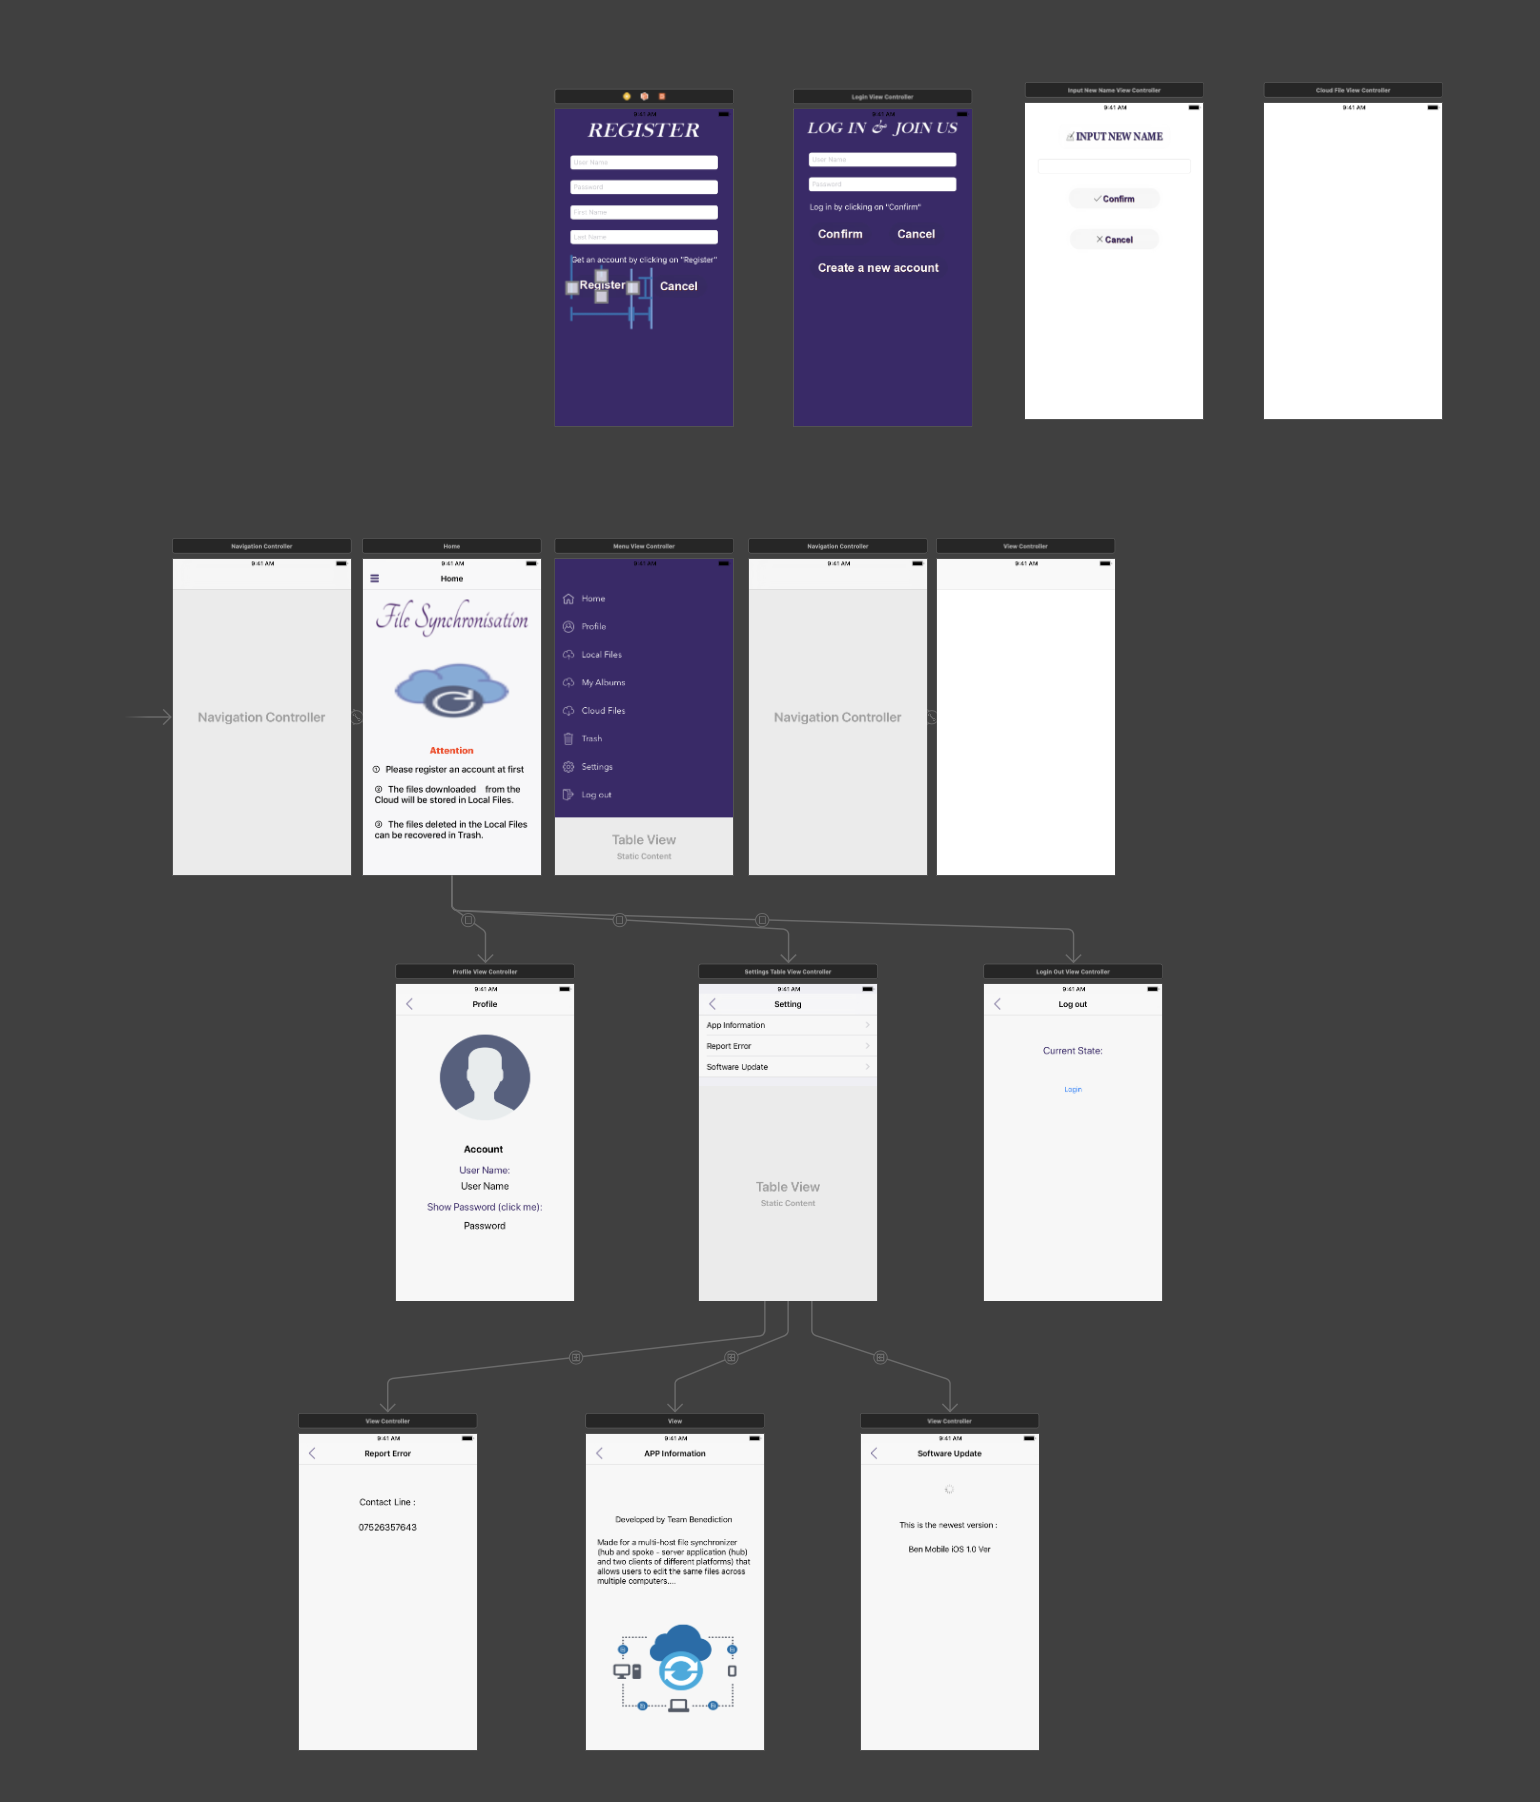
\includegraphics[width=6.3cm]{1111.png}
\end{center}
\caption{Hierarchical navigation in Main.storyboard}\label{ex777}
\end{figure}

Figure \ref{ex777} shows the hierarchical navigation in the Main.storyboard. There are five Xib files (custom views) that are not shown in storyboard. The Xib is used for implementing TableView and is actually embedded by coding methods in Main.storyboard, which allows the mobile client to provide a compatible overview for various iPhone models. This architecture is applied in pages of Local files, Cloud and Trash, with basic operations (download, upload, delete, rename) that can be handled by users. The users can upload documents to the server by choosing the file they want in the local memory.

In order to make the mobile application run smoothly, HTTP and Websocket are used to create a communication and file synchronization with the server. When the user trigger an operation, a HTTP request will be sent to the server and the server will send back the response messages (JSON) to the application. The JSON message will get decoded locally and saved as  a global public structured data. If there are any changes happening in server, it will multi-cast notifications via WebSocket to every client in the system. After receiving the notification, the mobile app will update the cloud files immediately and automatically. A synchronization button situated in the top of cloud page that supports manual update of the server files for users. The file conflict problems are also handled locally in the mobile application, where before the user triggers an operation to upload, update or delete a file, the file ID will be checked first and then a system latency is set for analyzing the information sent from the server (completion or error). 

\paragraph{User Interface}\mbox{} \\

The main page of the mobile client aims to provide directions for those who are not familiar with this app. A side menu shown in the left field of main page follows the strategy of hierarchical navigation, providing eight choices (\textbf{Welcome, Profile, Local Files, My Album, Cloud, Trash, Settings, Login/Logout}) for users to reach a destination, which will be addressed in more details in this section. 

The interface introduction begins with the Cloud page that shows all the files in the server. Users are not allowed to manipulate cloud files until they have logged in successfully. Security and confidentiality are two of the main issues that both the client and the server want to address in the program to prevent information leakage during the period of data transmission, otherwise, without authentication, all the communications based on HTTP request will be forbidden by the server. Figure \ref{fig:f5}, \ref{fig:f6}, \ref{fig:f7} and \ref{fig:f8} shown below gives a brief overview of the login and register design.

\begin{figure}[H]
  \centering
  \subfloat[User Status]{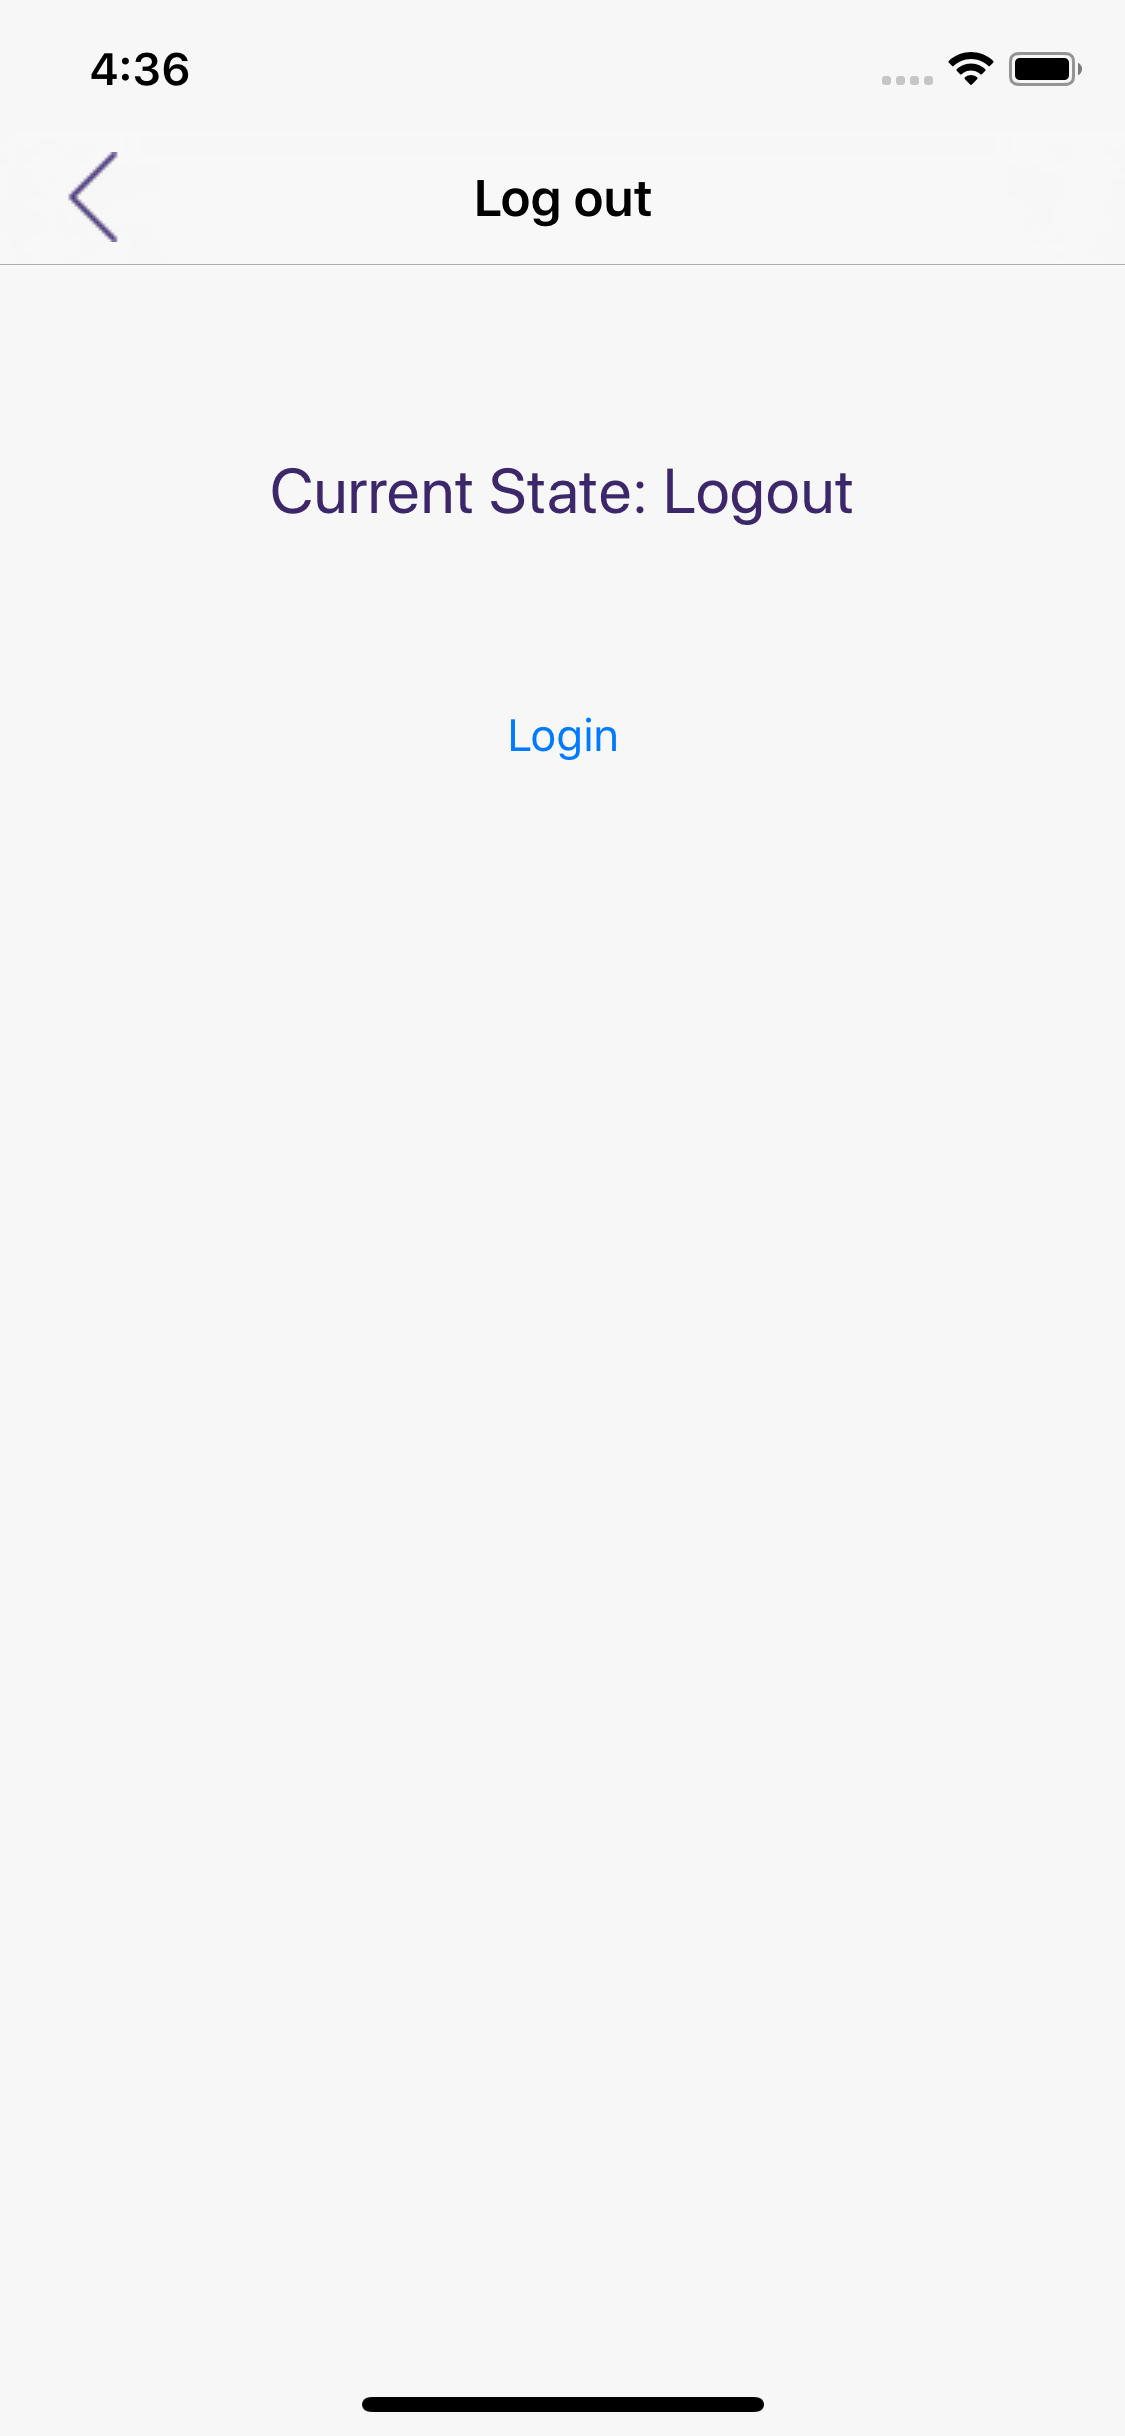
\includegraphics[width=0.19\textwidth]{2.png}\label{fig:f5}}
  \hfill
  \subfloat[Log In]{
\includegraphics[width=0.19\textwidth]{3.png}\label{fig:f6}}
  \hfill
  \subfloat[Login Successfully]{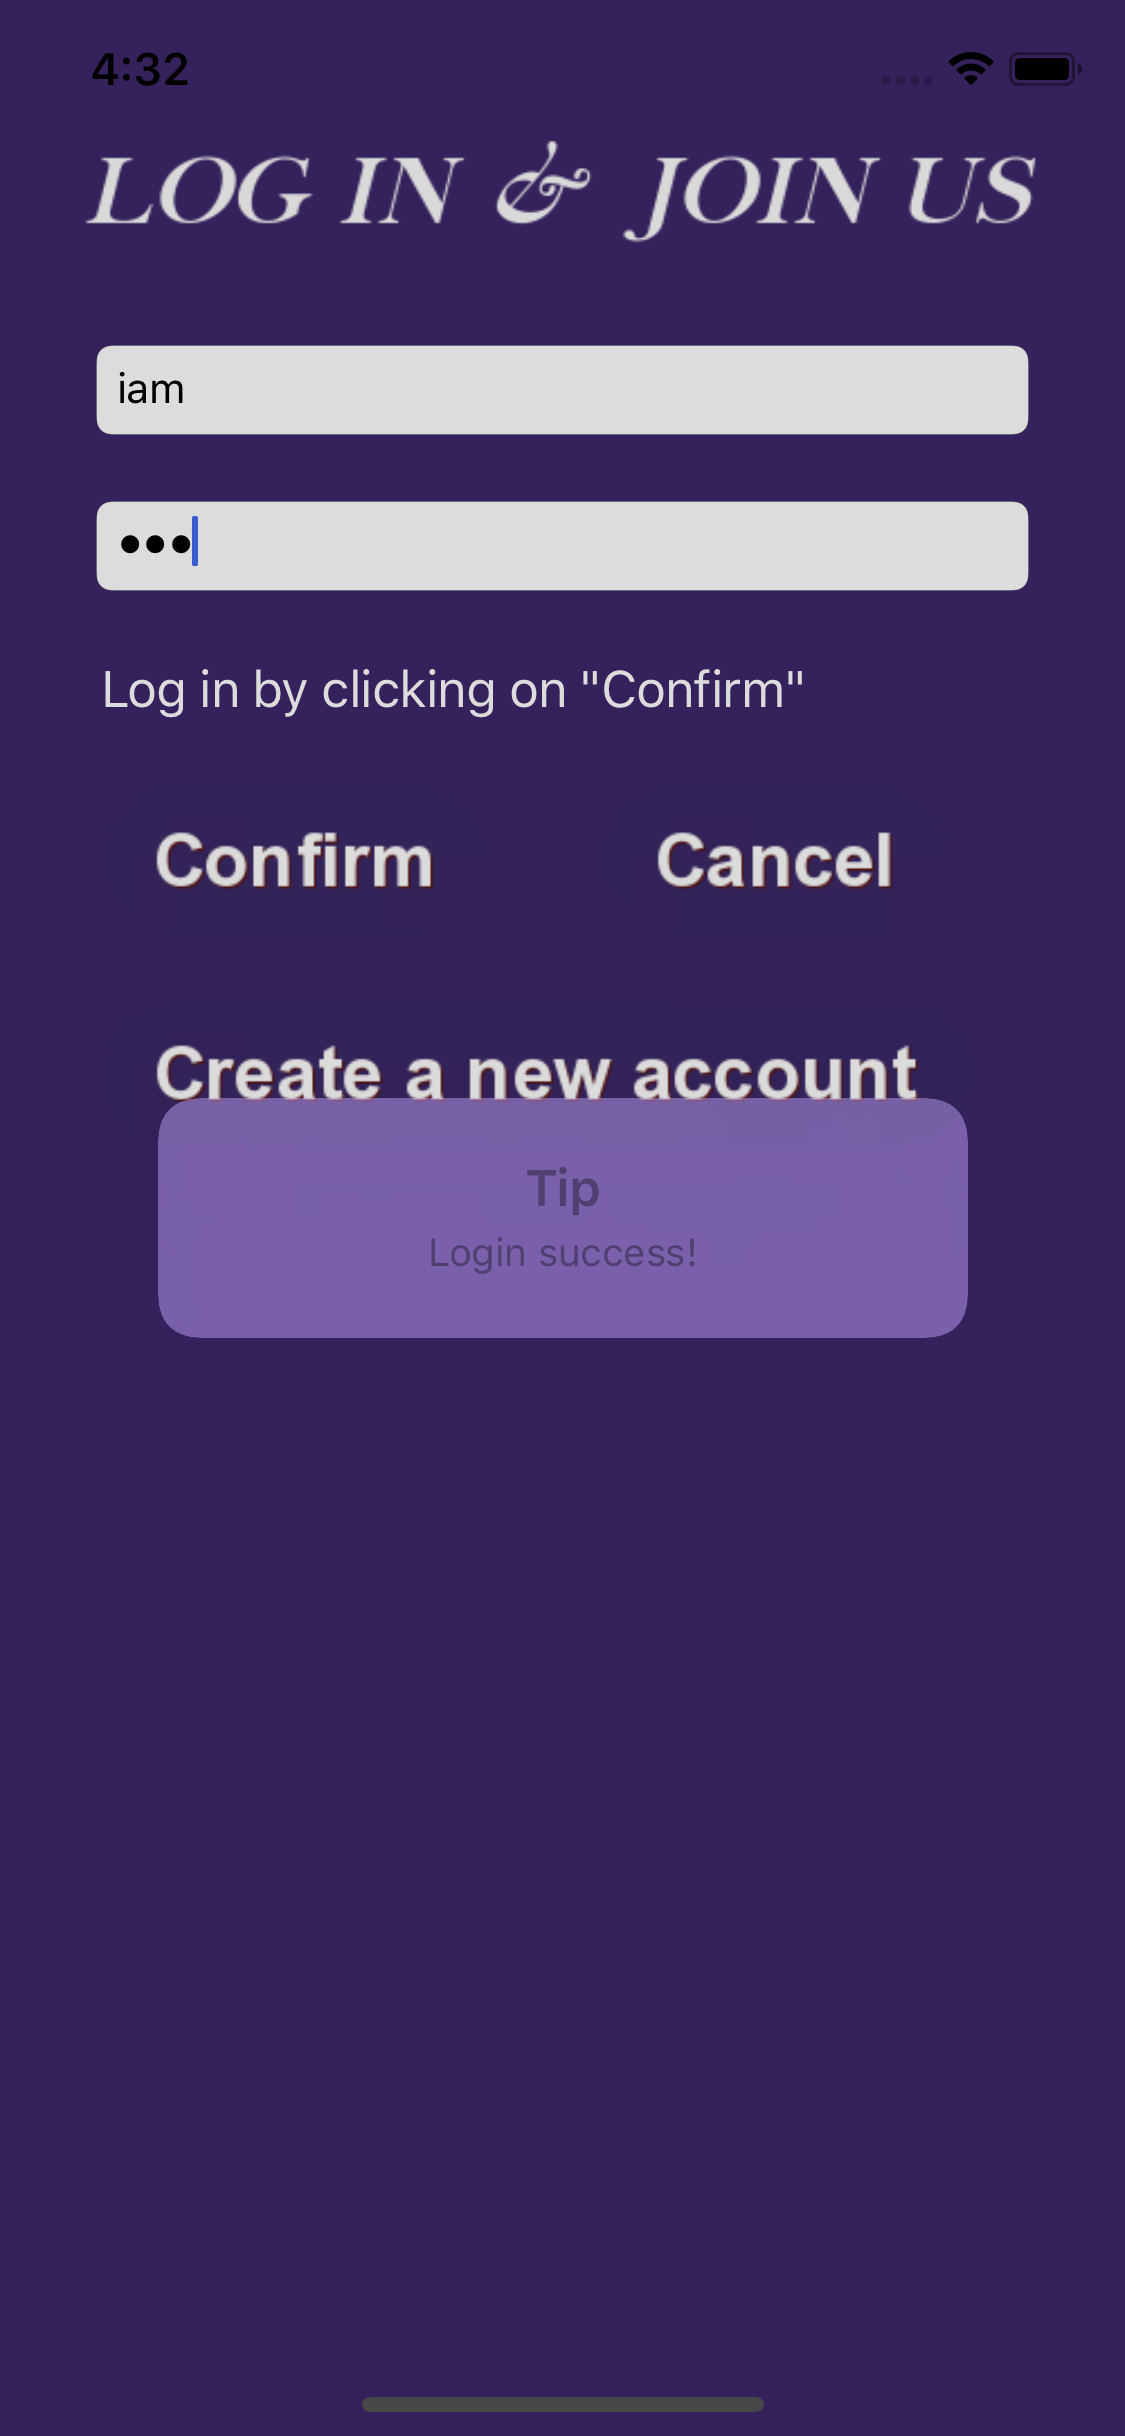
\includegraphics[width=0.19\textwidth]{4.png}\label{fig:f7}}
  \hfill
  \subfloat[Register Successfully]{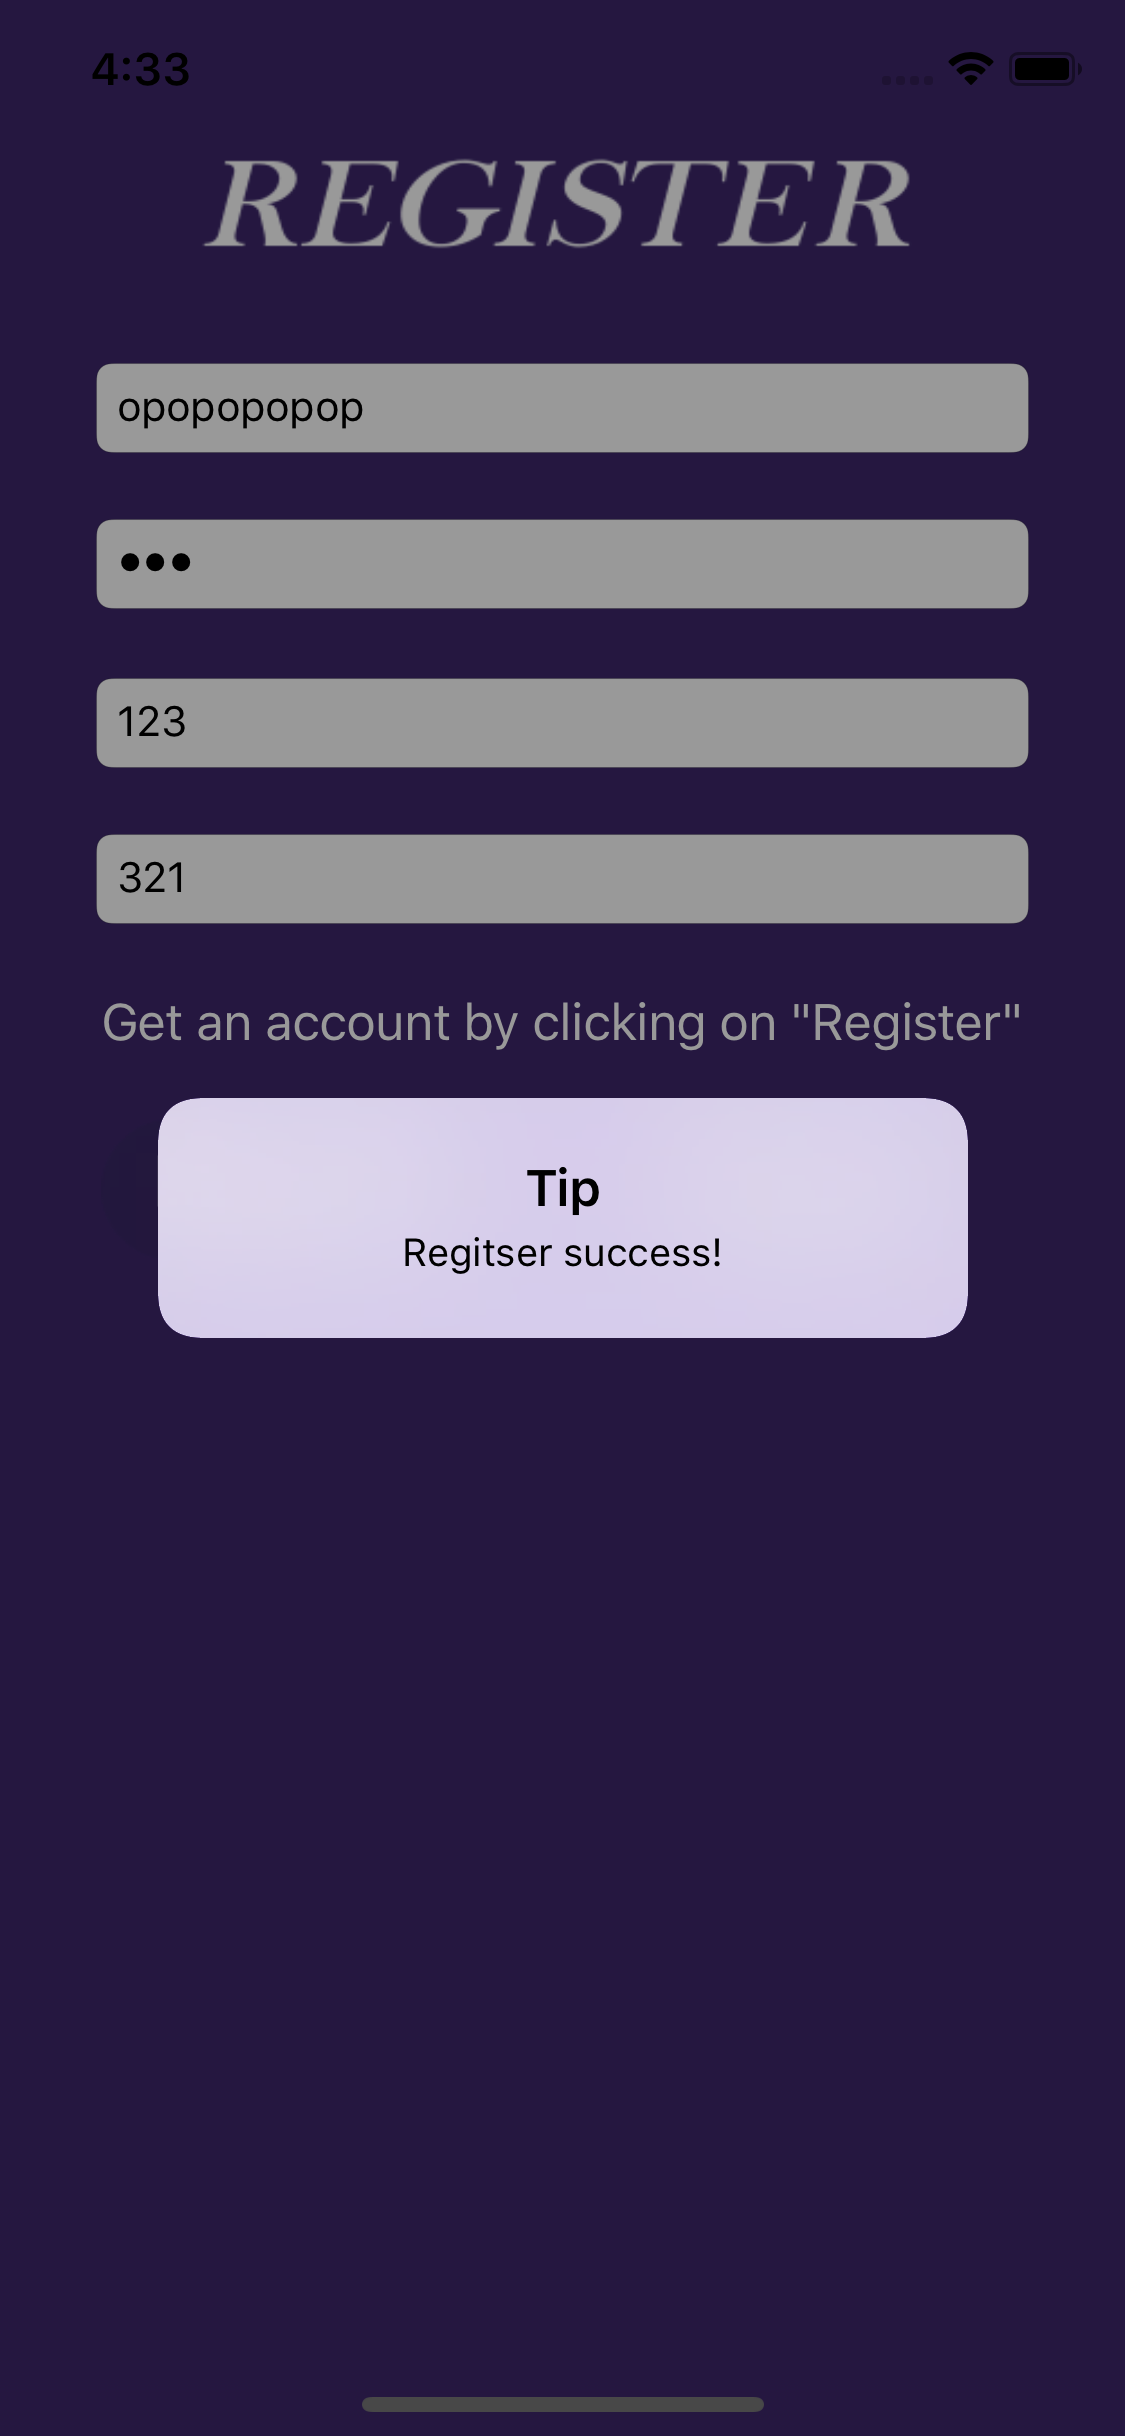
\includegraphics[width=0.19\textwidth]{5.png}\label{fig:f8}}
  \caption{Login and register in mobile client}
\end{figure}


The Profile page contains information about the current user. The user can choose to make the password visible or invisible (both of username and password are messages sent by the server after logging in successfully). Figure \ref{fig:example} shows the profile interface deisgn.

\begin{figure}[H]
    \centering
    \subfloat[Password visible]{{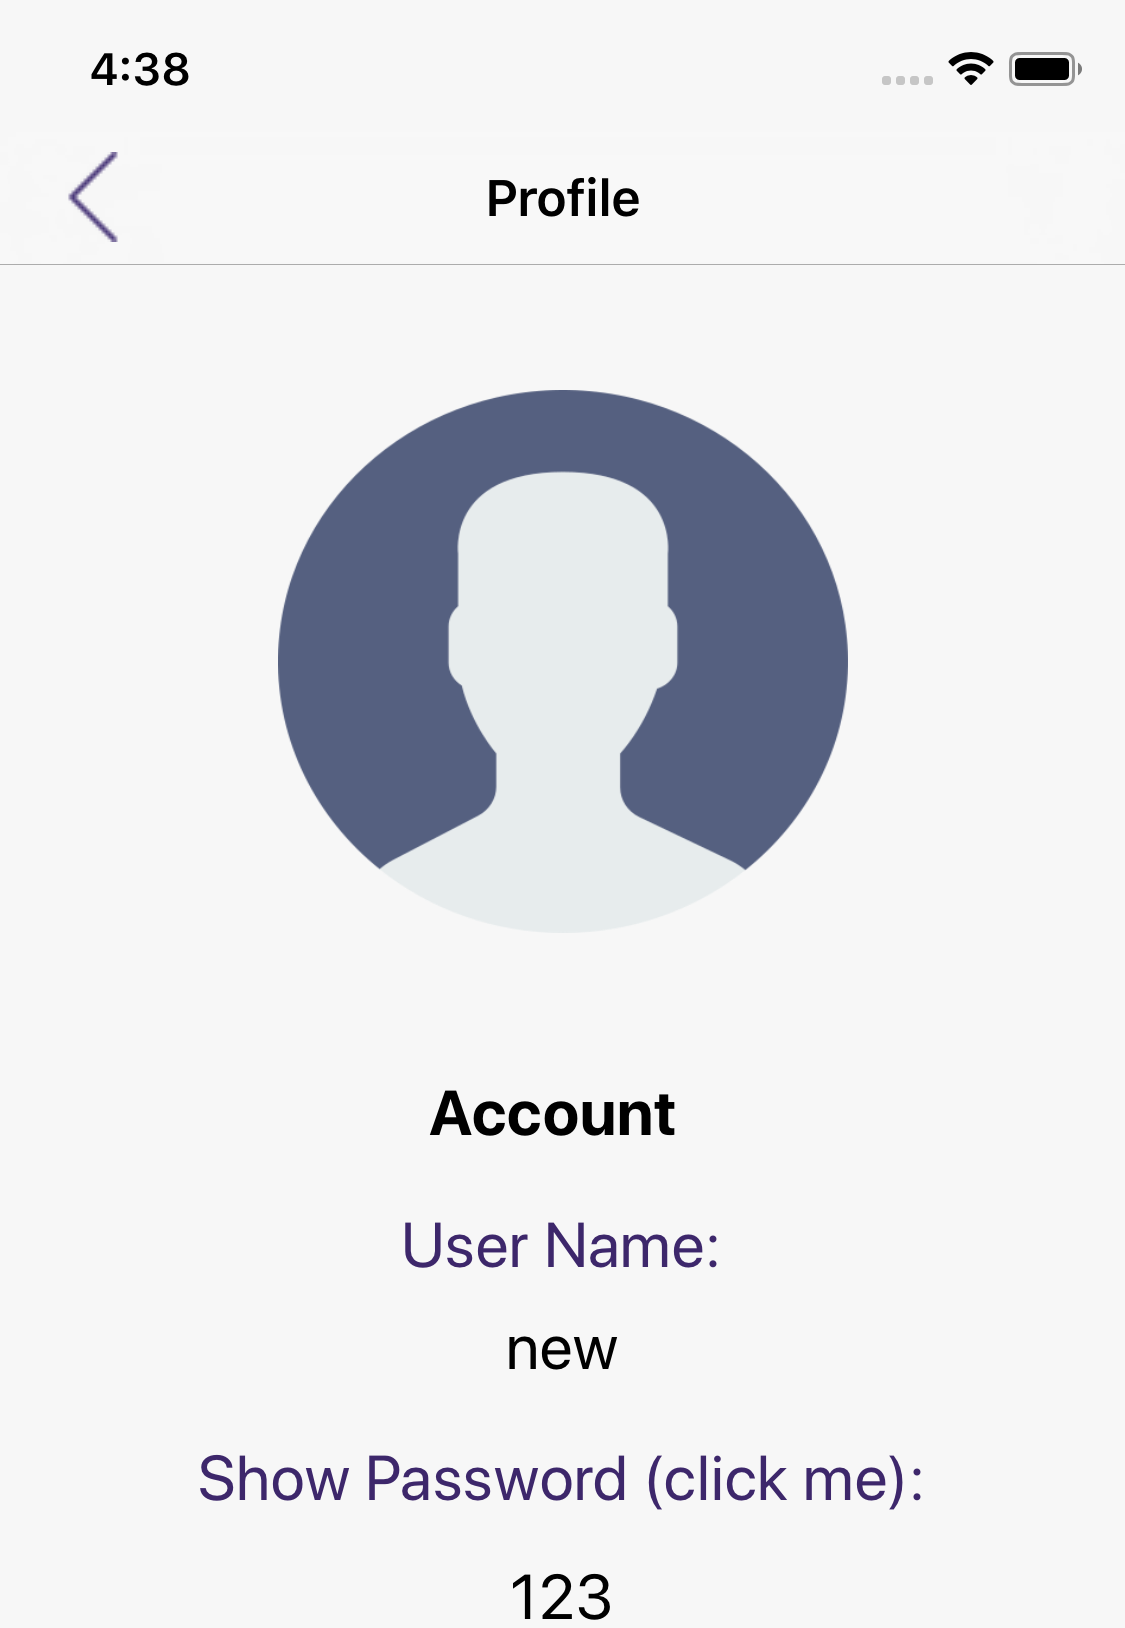
\includegraphics[width=3cm]{7.png}}}
    \qquad
    \subfloat[Password invisible]{{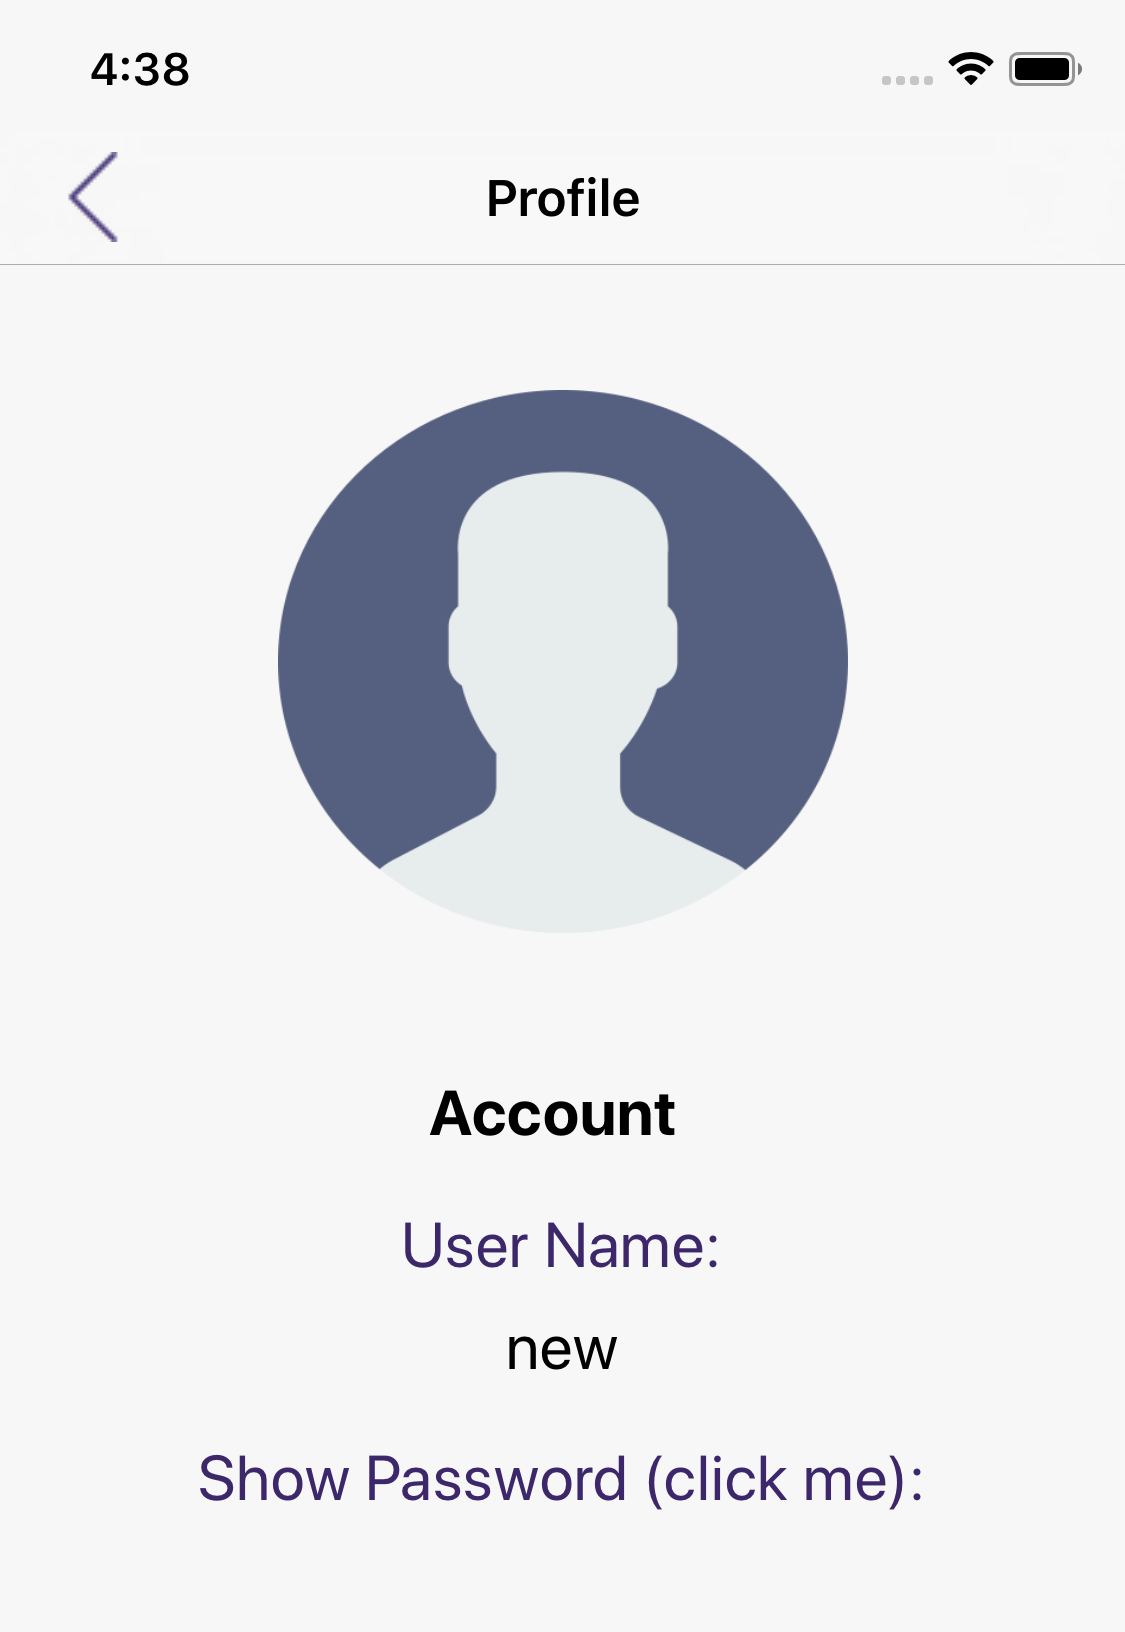
\includegraphics[width=3cm]{8.png}}}
    \caption{User Profile}%
    \label{fig:example}%
\end{figure}

Next, the Local Files page gives the user access to files that are saved locally, this will be done by creating a local directory to store the files downloaded from the server. The user will be able to slide the table view cell from right to left and 3 buttons should appear for Upload, Rename and Delete to trigger the operations on the local file. The team follows the rules of flat interface design, where Upload means that the user can upload a local file to the server, Rename is the function to change the file name locally and Delete is for deleting a file where this file will be moved to Trash where a new directory will be created for saving deleted documents from the local files. On the top of Cloud, Local files and Trash, a search bar can be found for searching files' name. The mobile client will be able to provide a preview of various file format, including rtf, doc, zip, png, gif, mp4, mp3, jpg, txt and so on. Figure \ref{fig:f1}, \ref{fig:f2}, \ref{fig:f3} and \ref{fig:f4} shown below demonstrate the fundamental functions of TableView in mobile client. Figure \ref{fig:f10}, \ref{fig:f11}, \ref{fig:f12} and \ref{fig:f13} displays the operations that can be done in Local Files and Cloud Files.


\begin{figure}[H]
  \centering
  \subfloat[Local files]{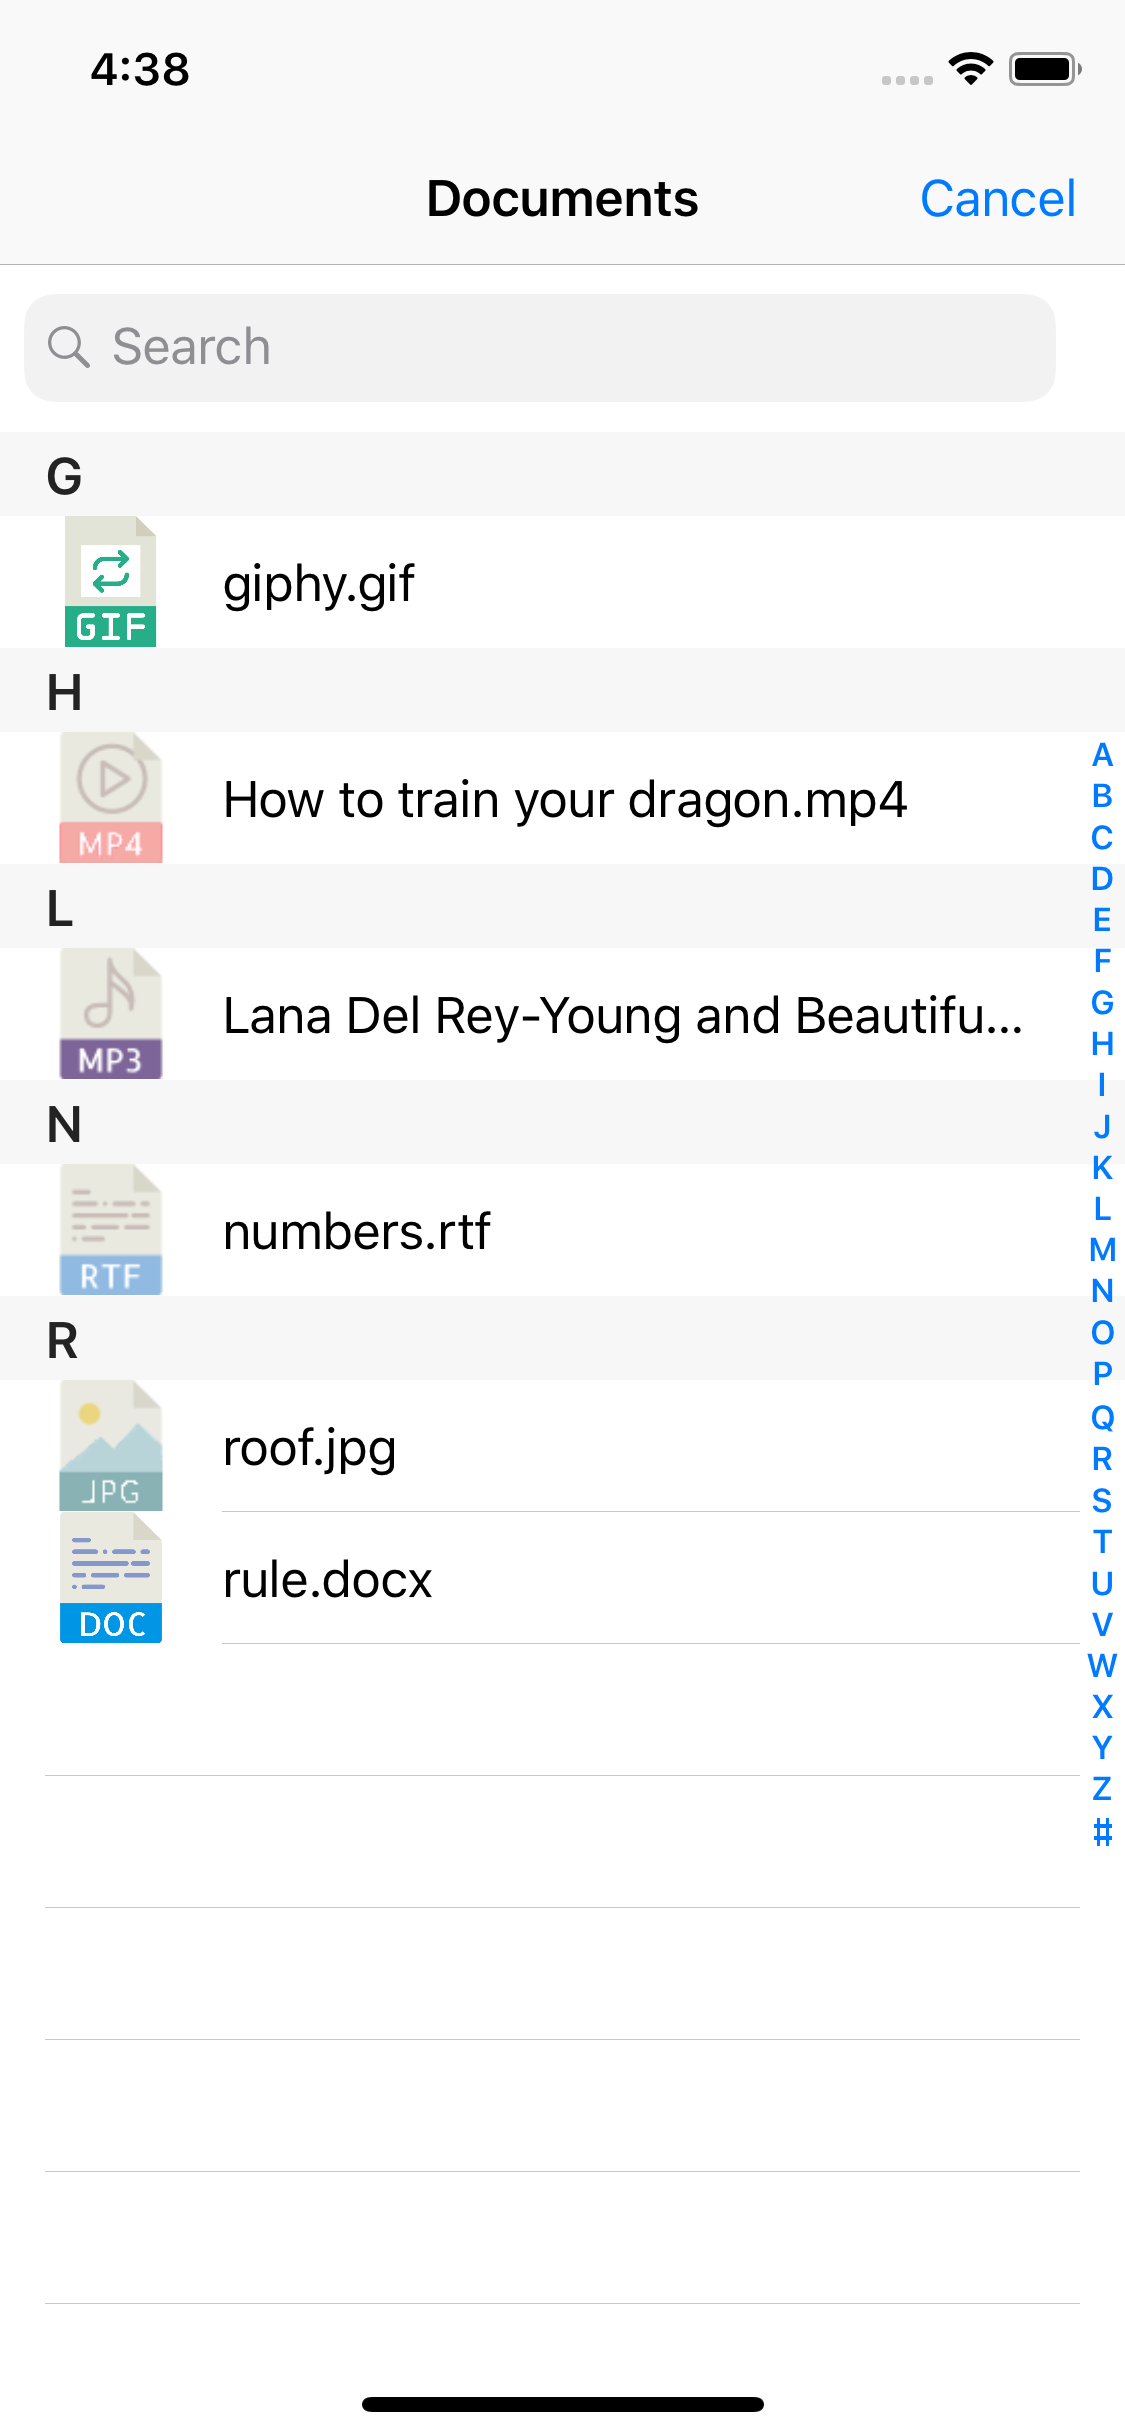
\includegraphics[width=0.19\textwidth]{9.png}\label{fig:f1}}
  \hfill
  \subfloat[Playing MP4]{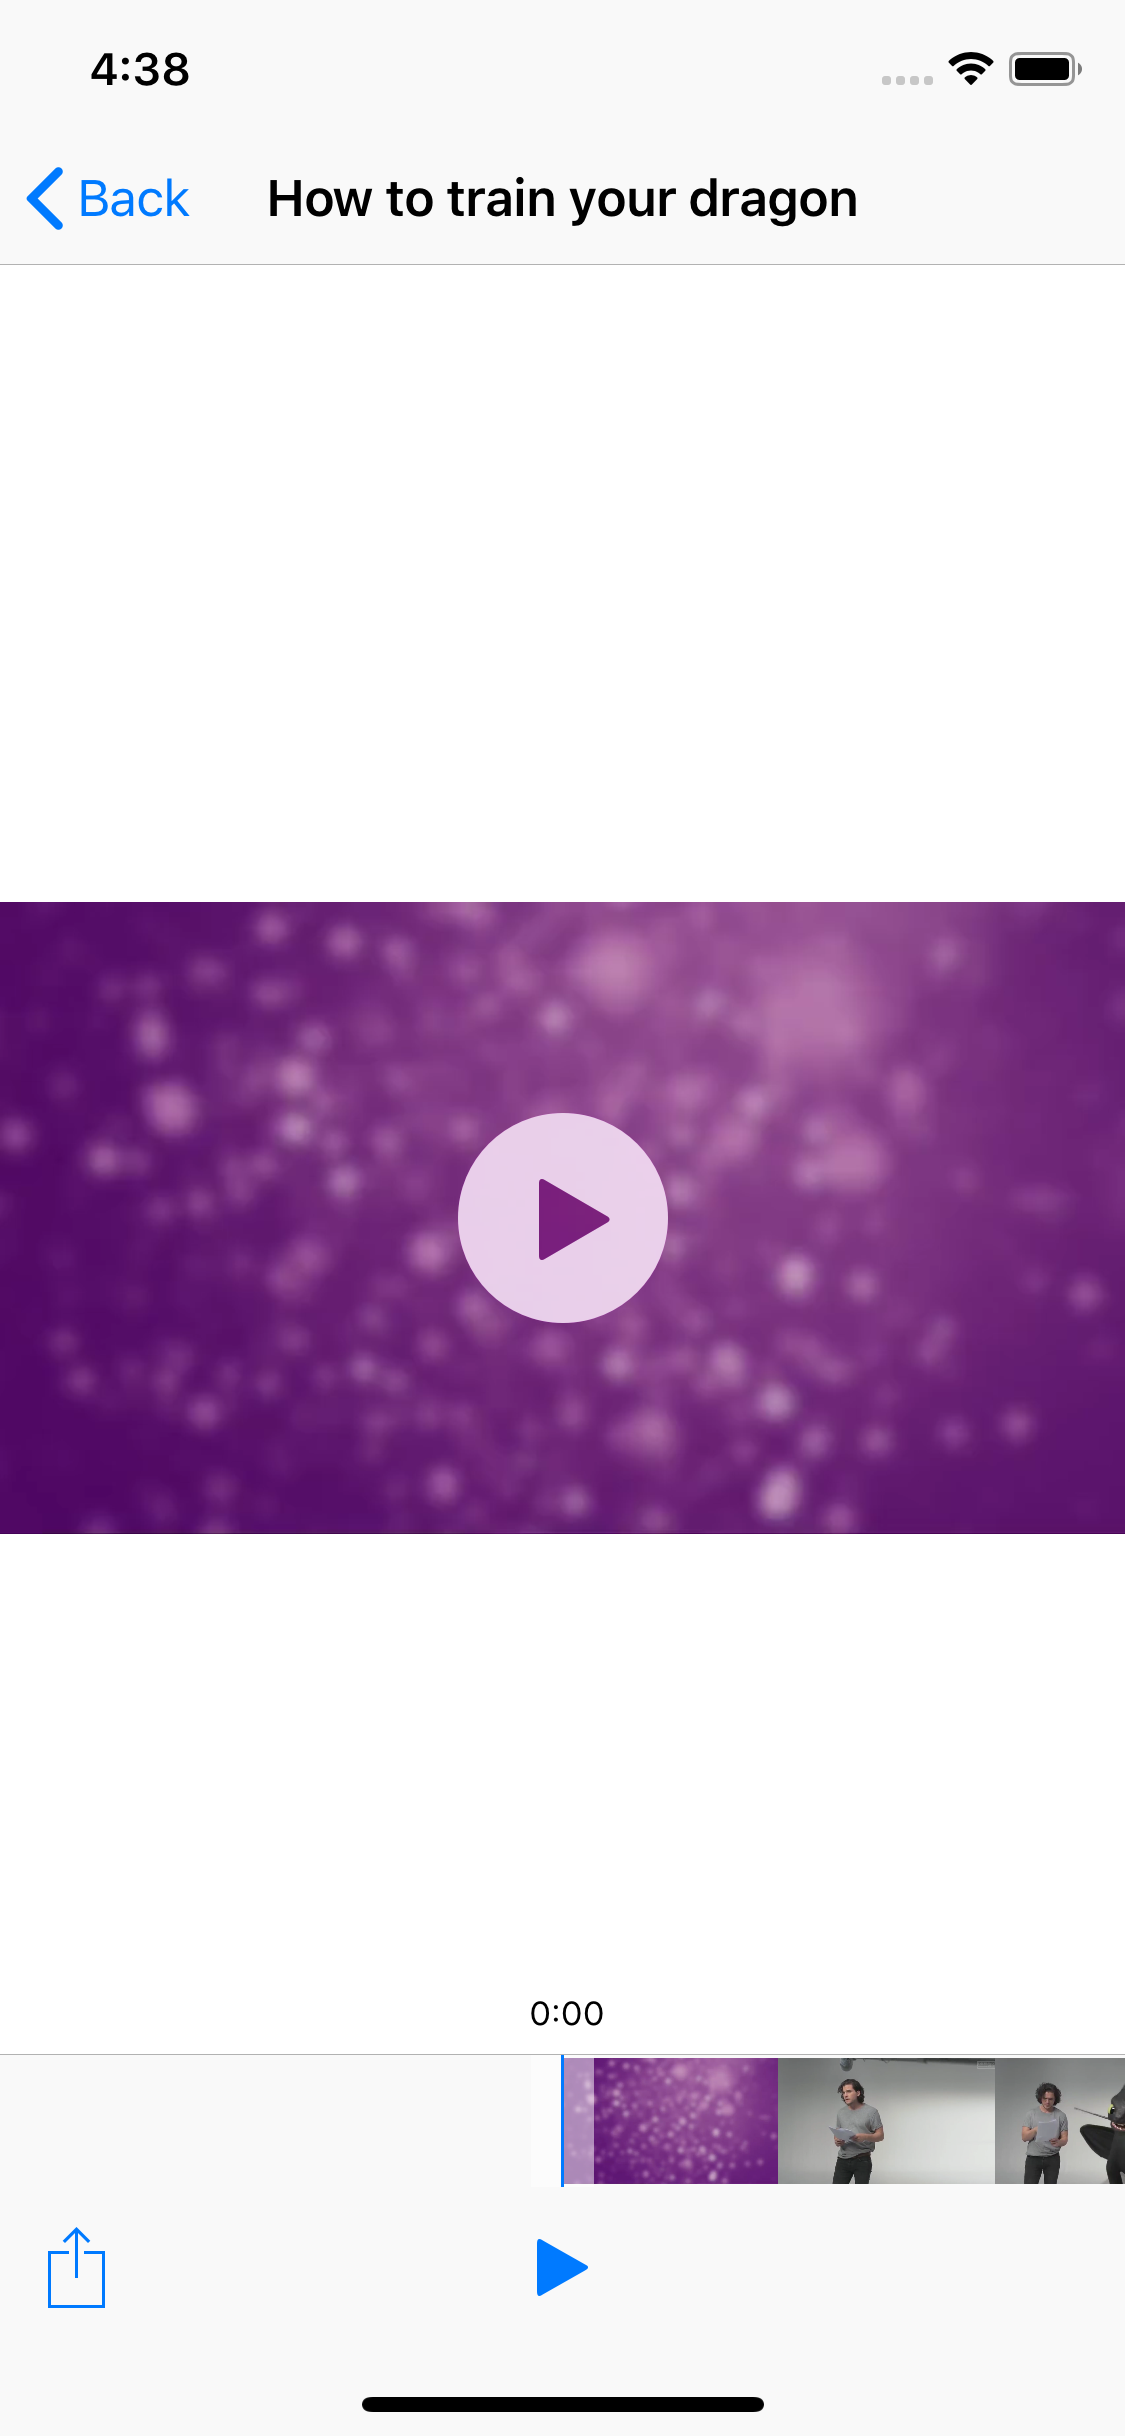
\includegraphics[width=0.19\textwidth]{10.png}\label{fig:f2}}
  \hfill
  \subfloat[Playing MP3]{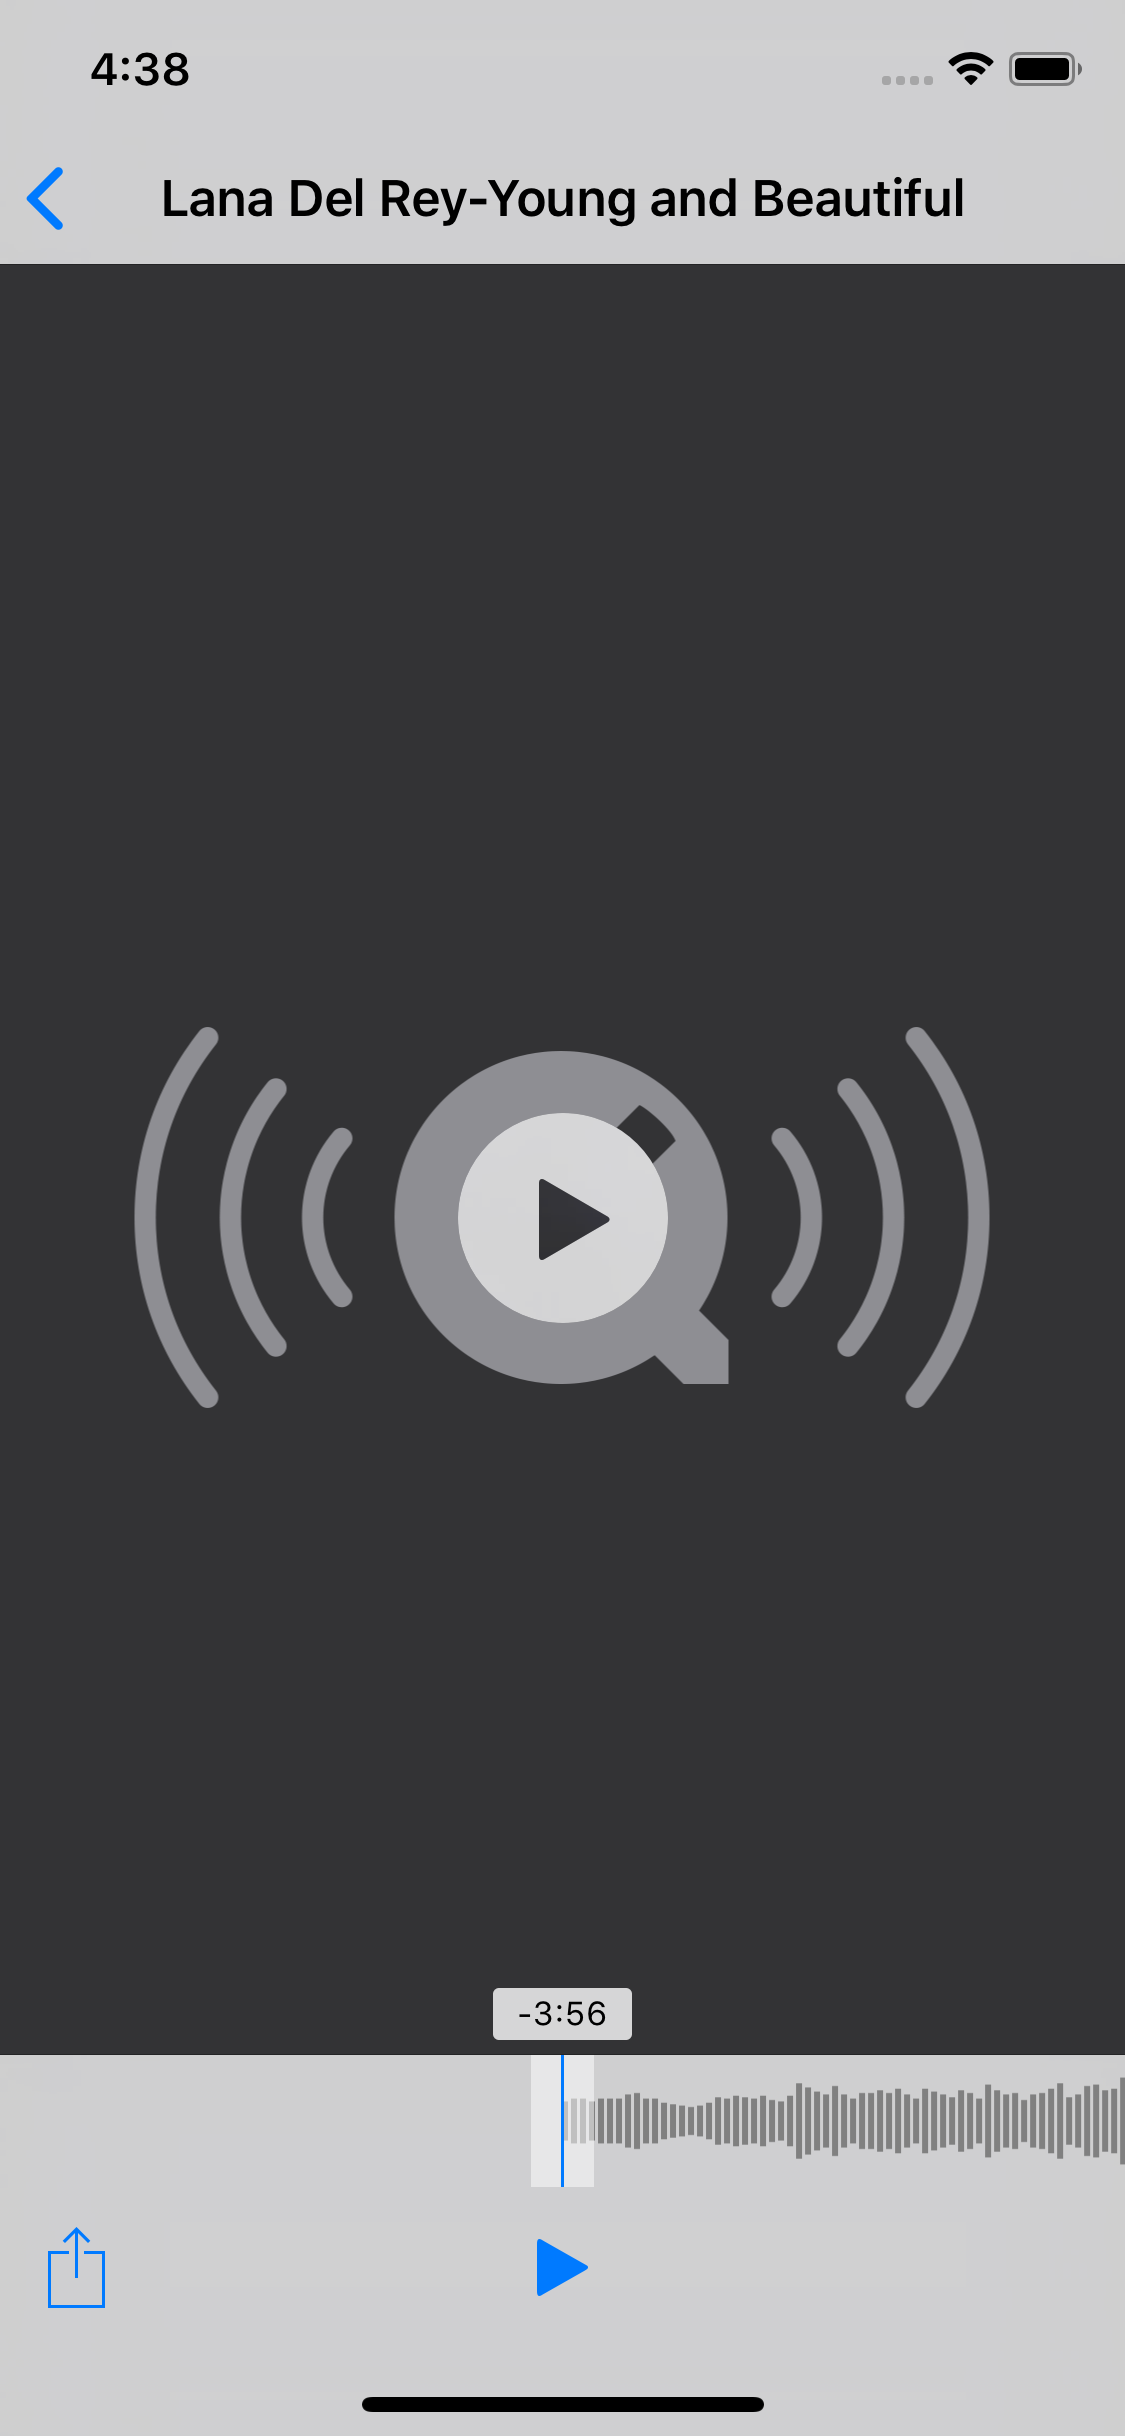
\includegraphics[width=0.19\textwidth]{11.png}\label{fig:f3}}
  \hfill
  \subfloat[Search a file]{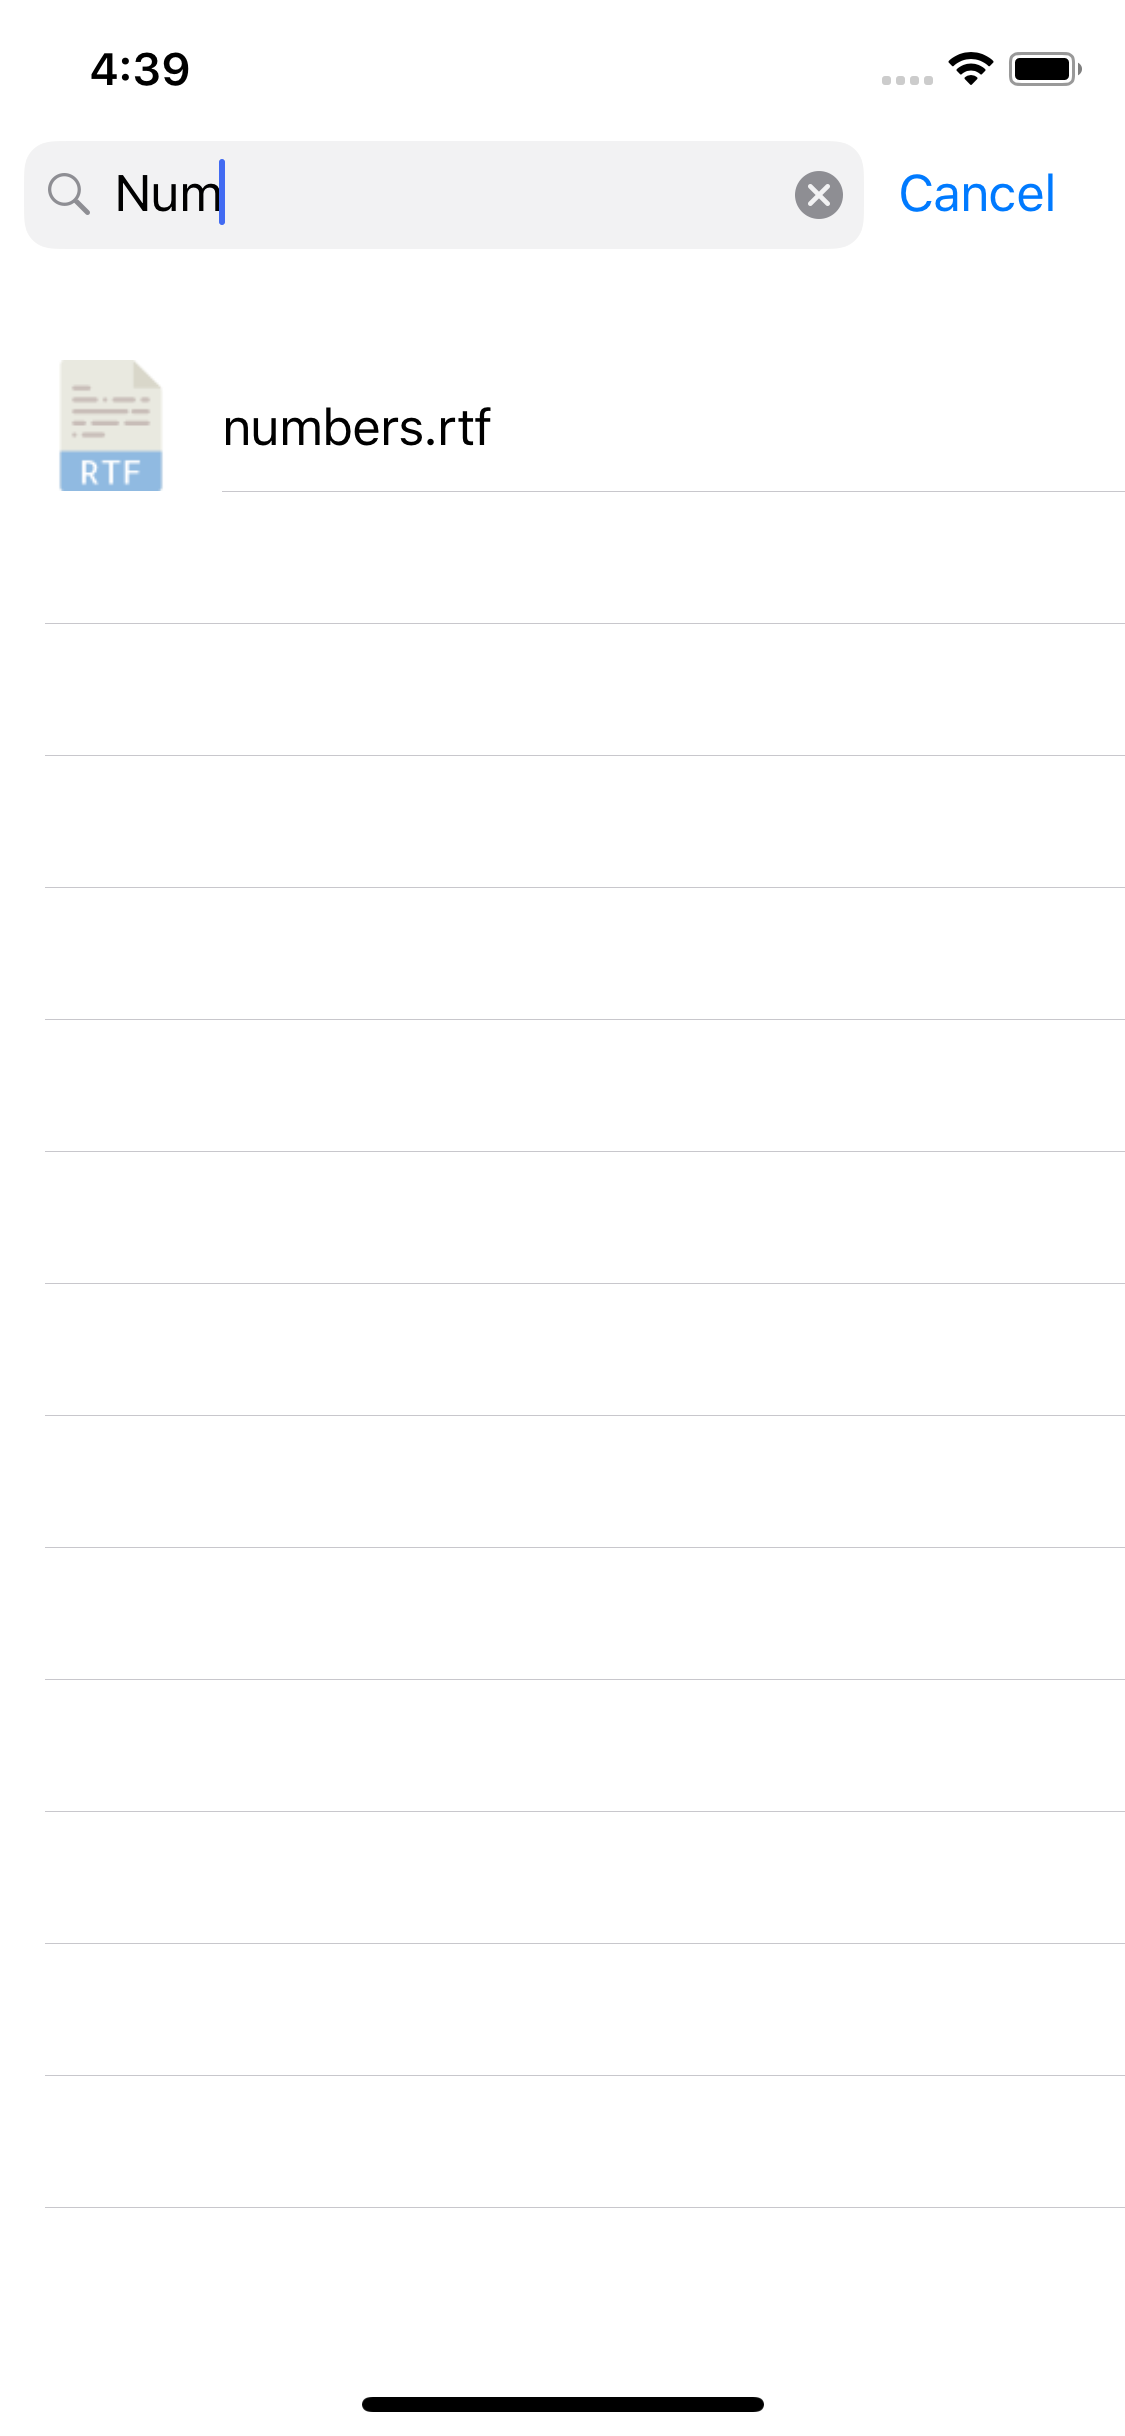
\includegraphics[width=0.19\textwidth]{12.png}\label{fig:f4}}
  \caption{TableView functions}
\end{figure}

\begin{figure}[H]
  \centering
  \subfloat[Local files]{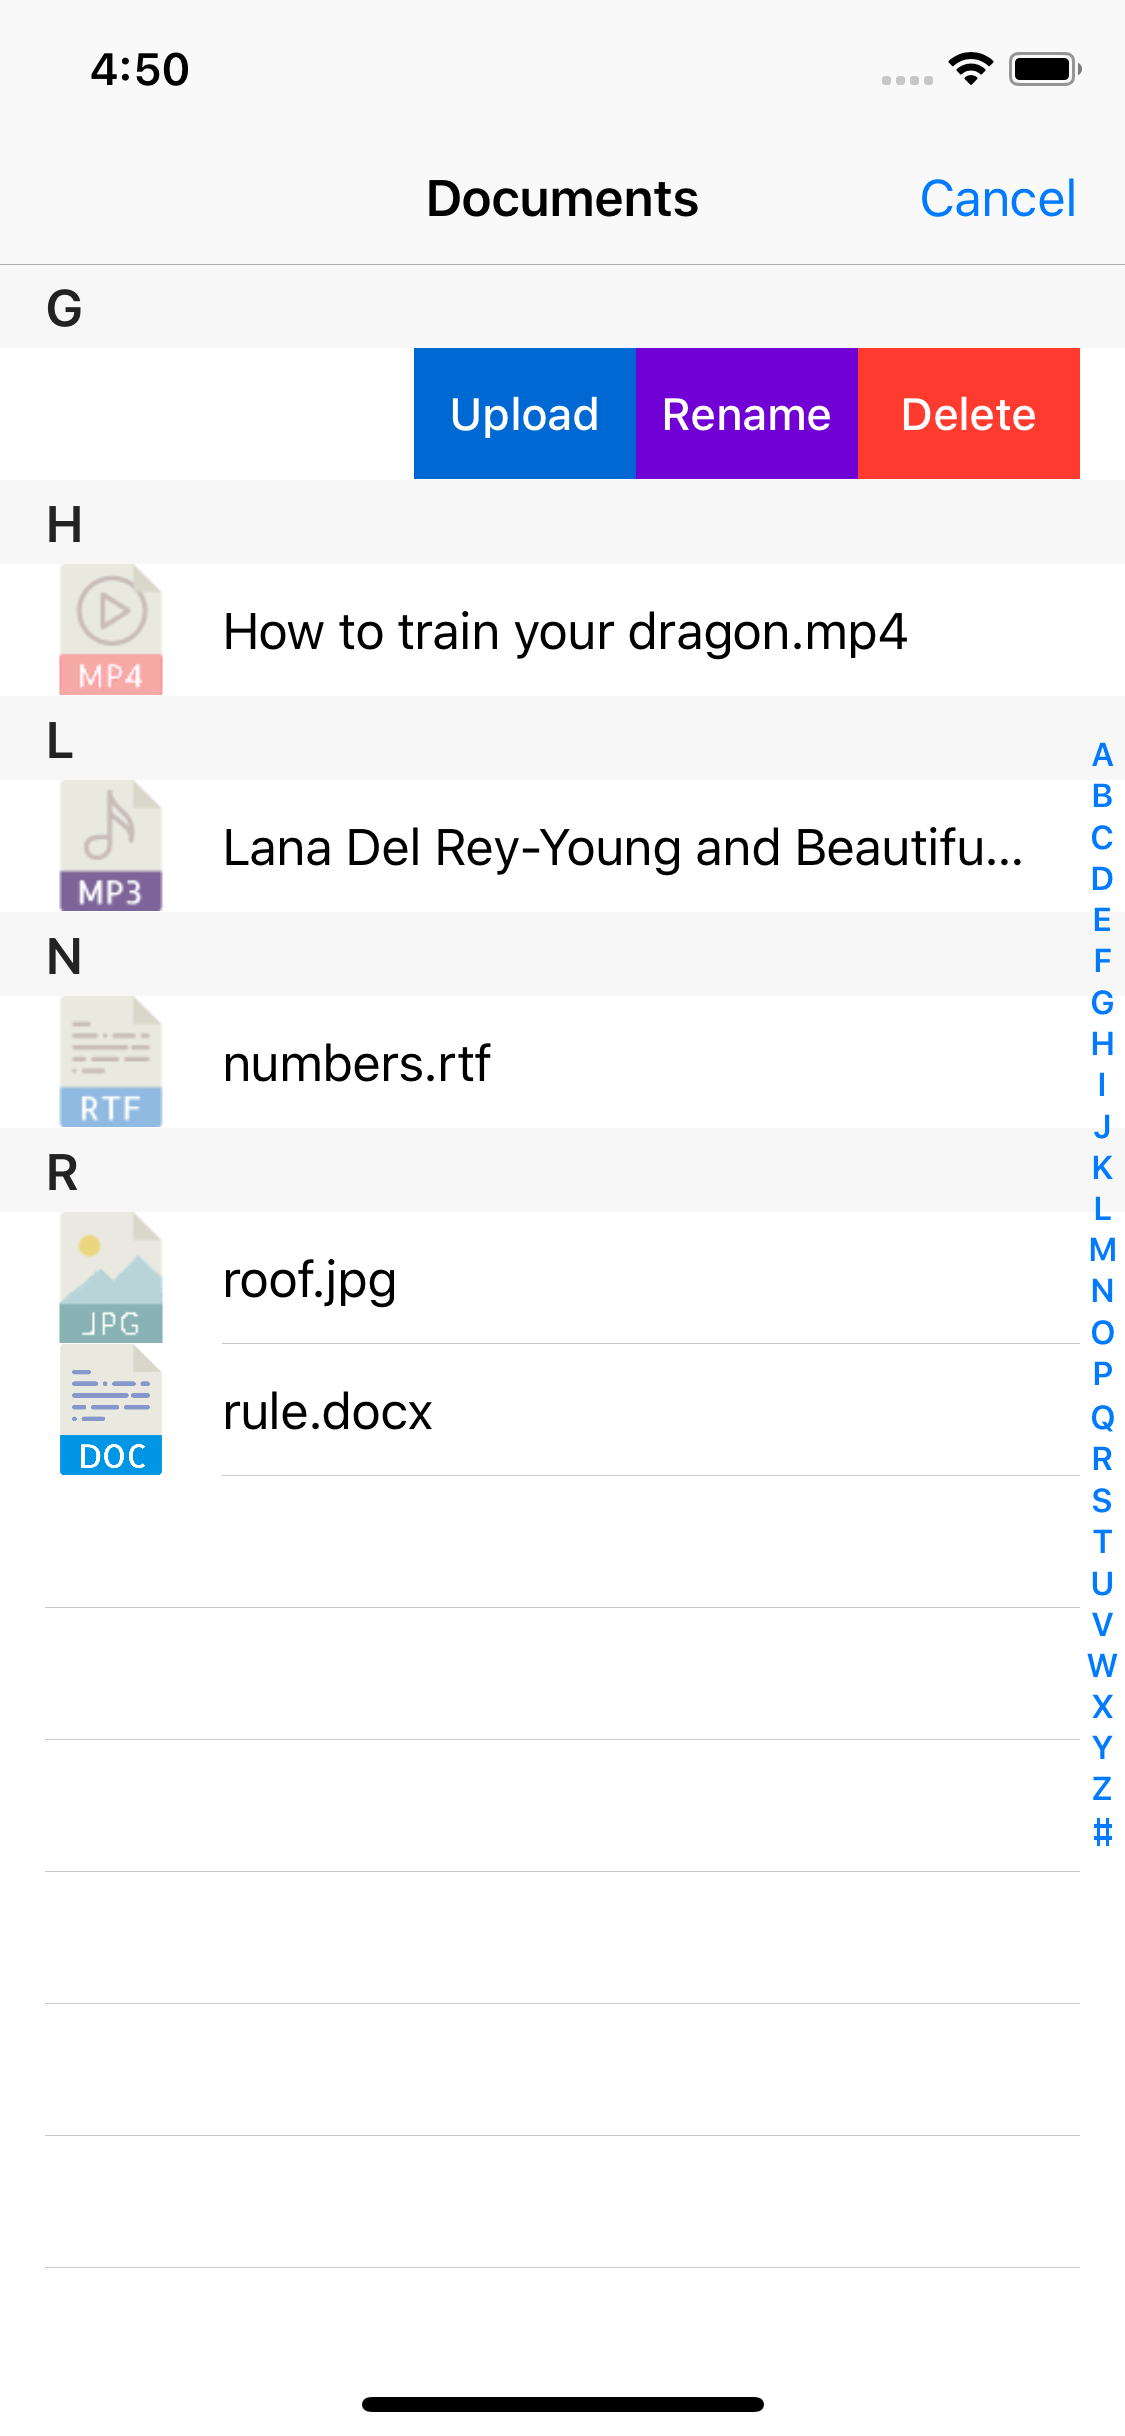
\includegraphics[width=0.19\textwidth]{16.png}\label{fig:f10}}
  \hfill
  \subfloat[Rename]{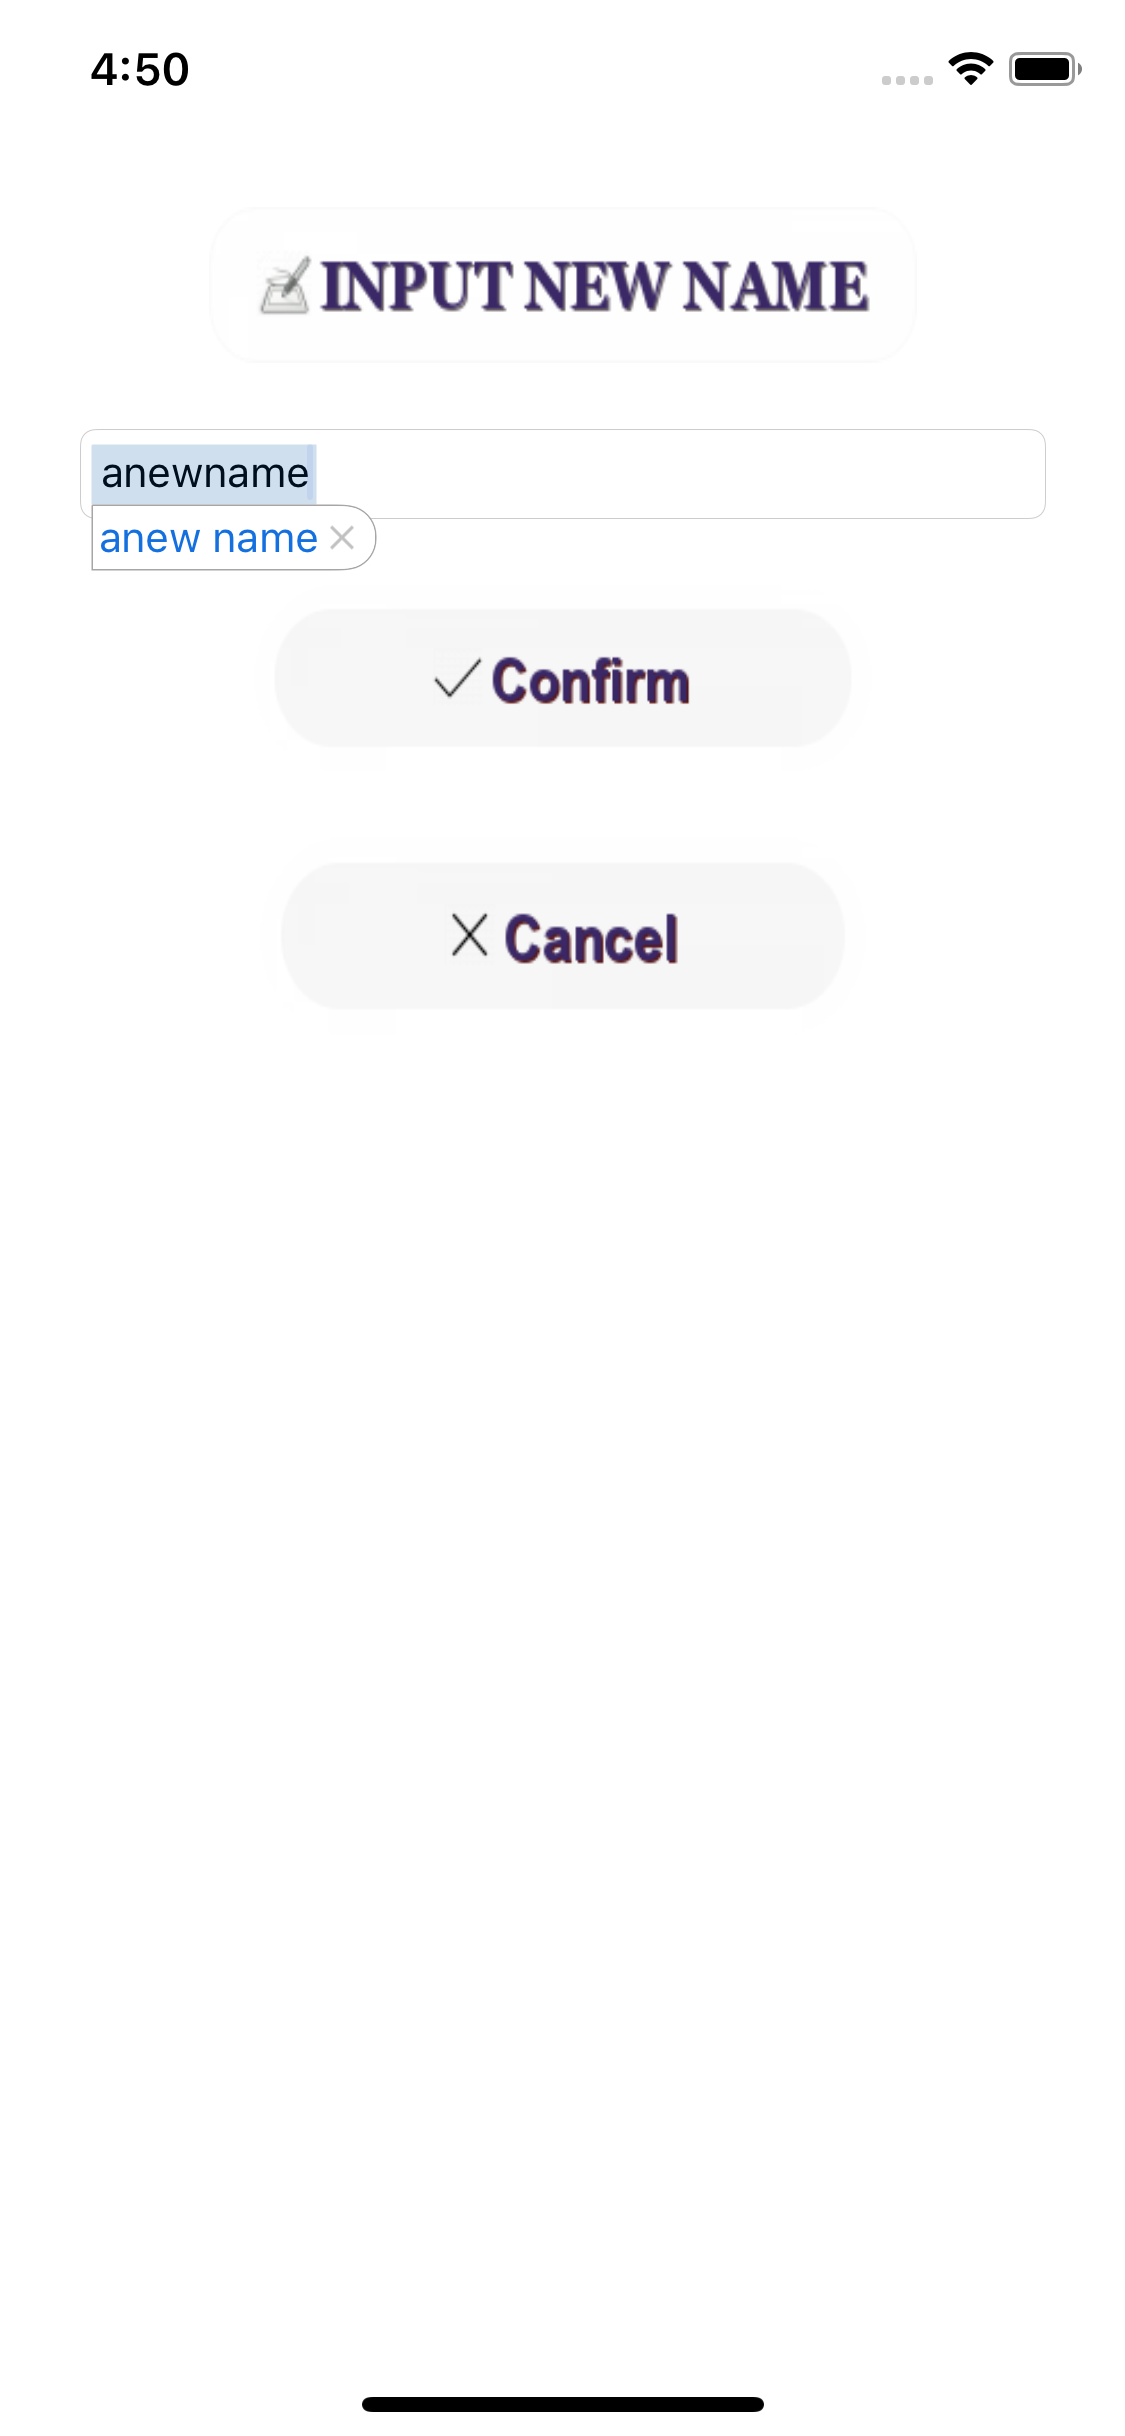
\includegraphics[width=0.19\textwidth]{17.png}\label{fig:f11}}
  \hfill
  \subfloat[Multi-select files]{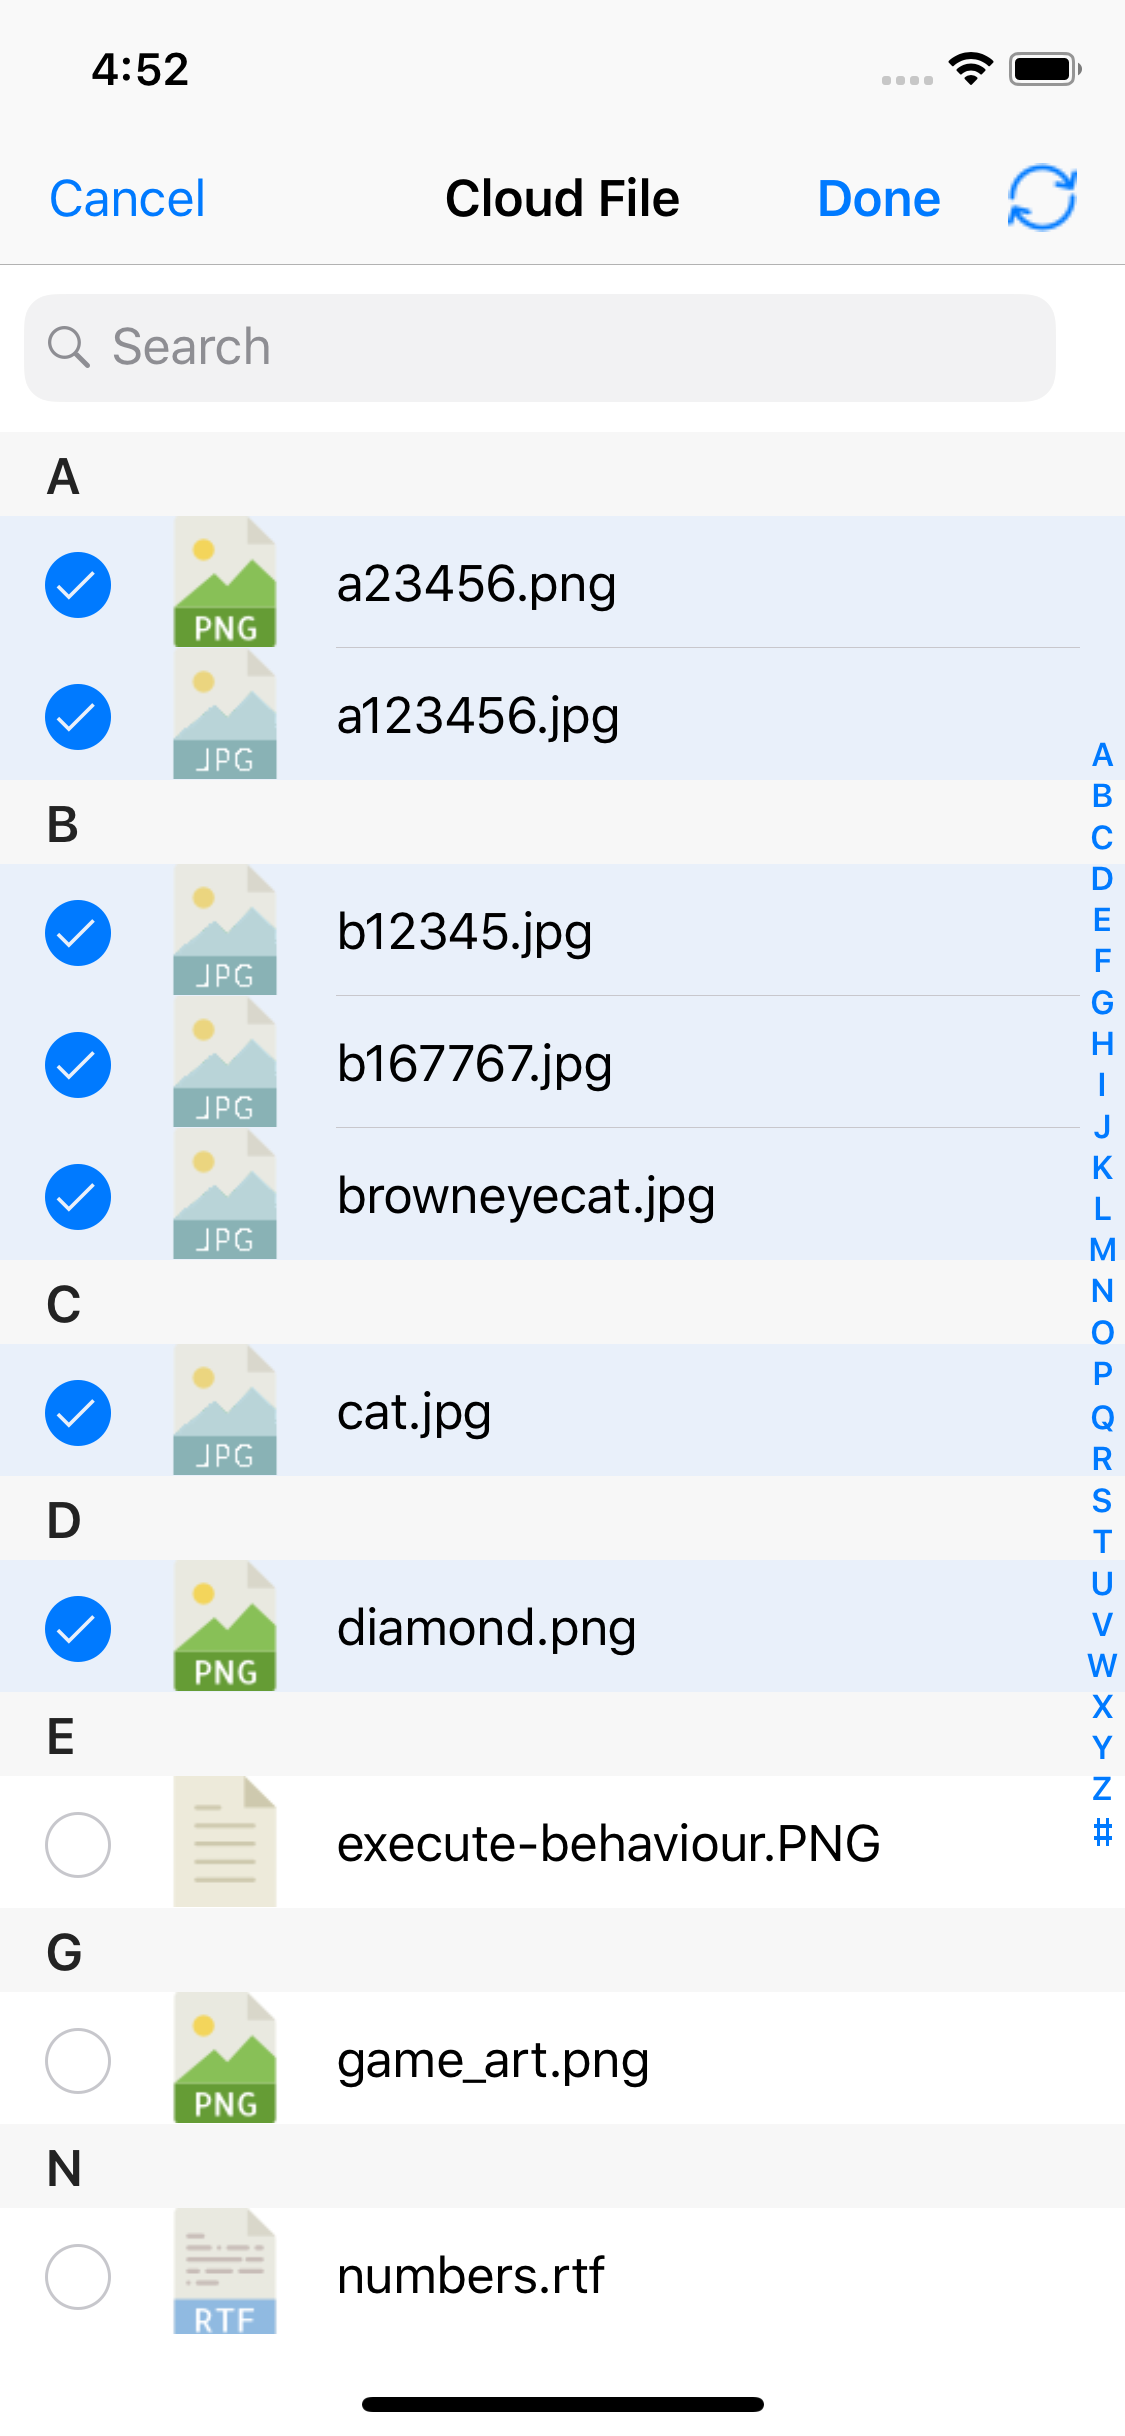
\includegraphics[width=0.19\textwidth]{23.png}\label{fig:f12}}
  \hfill
  \subfloat[Cloud files]{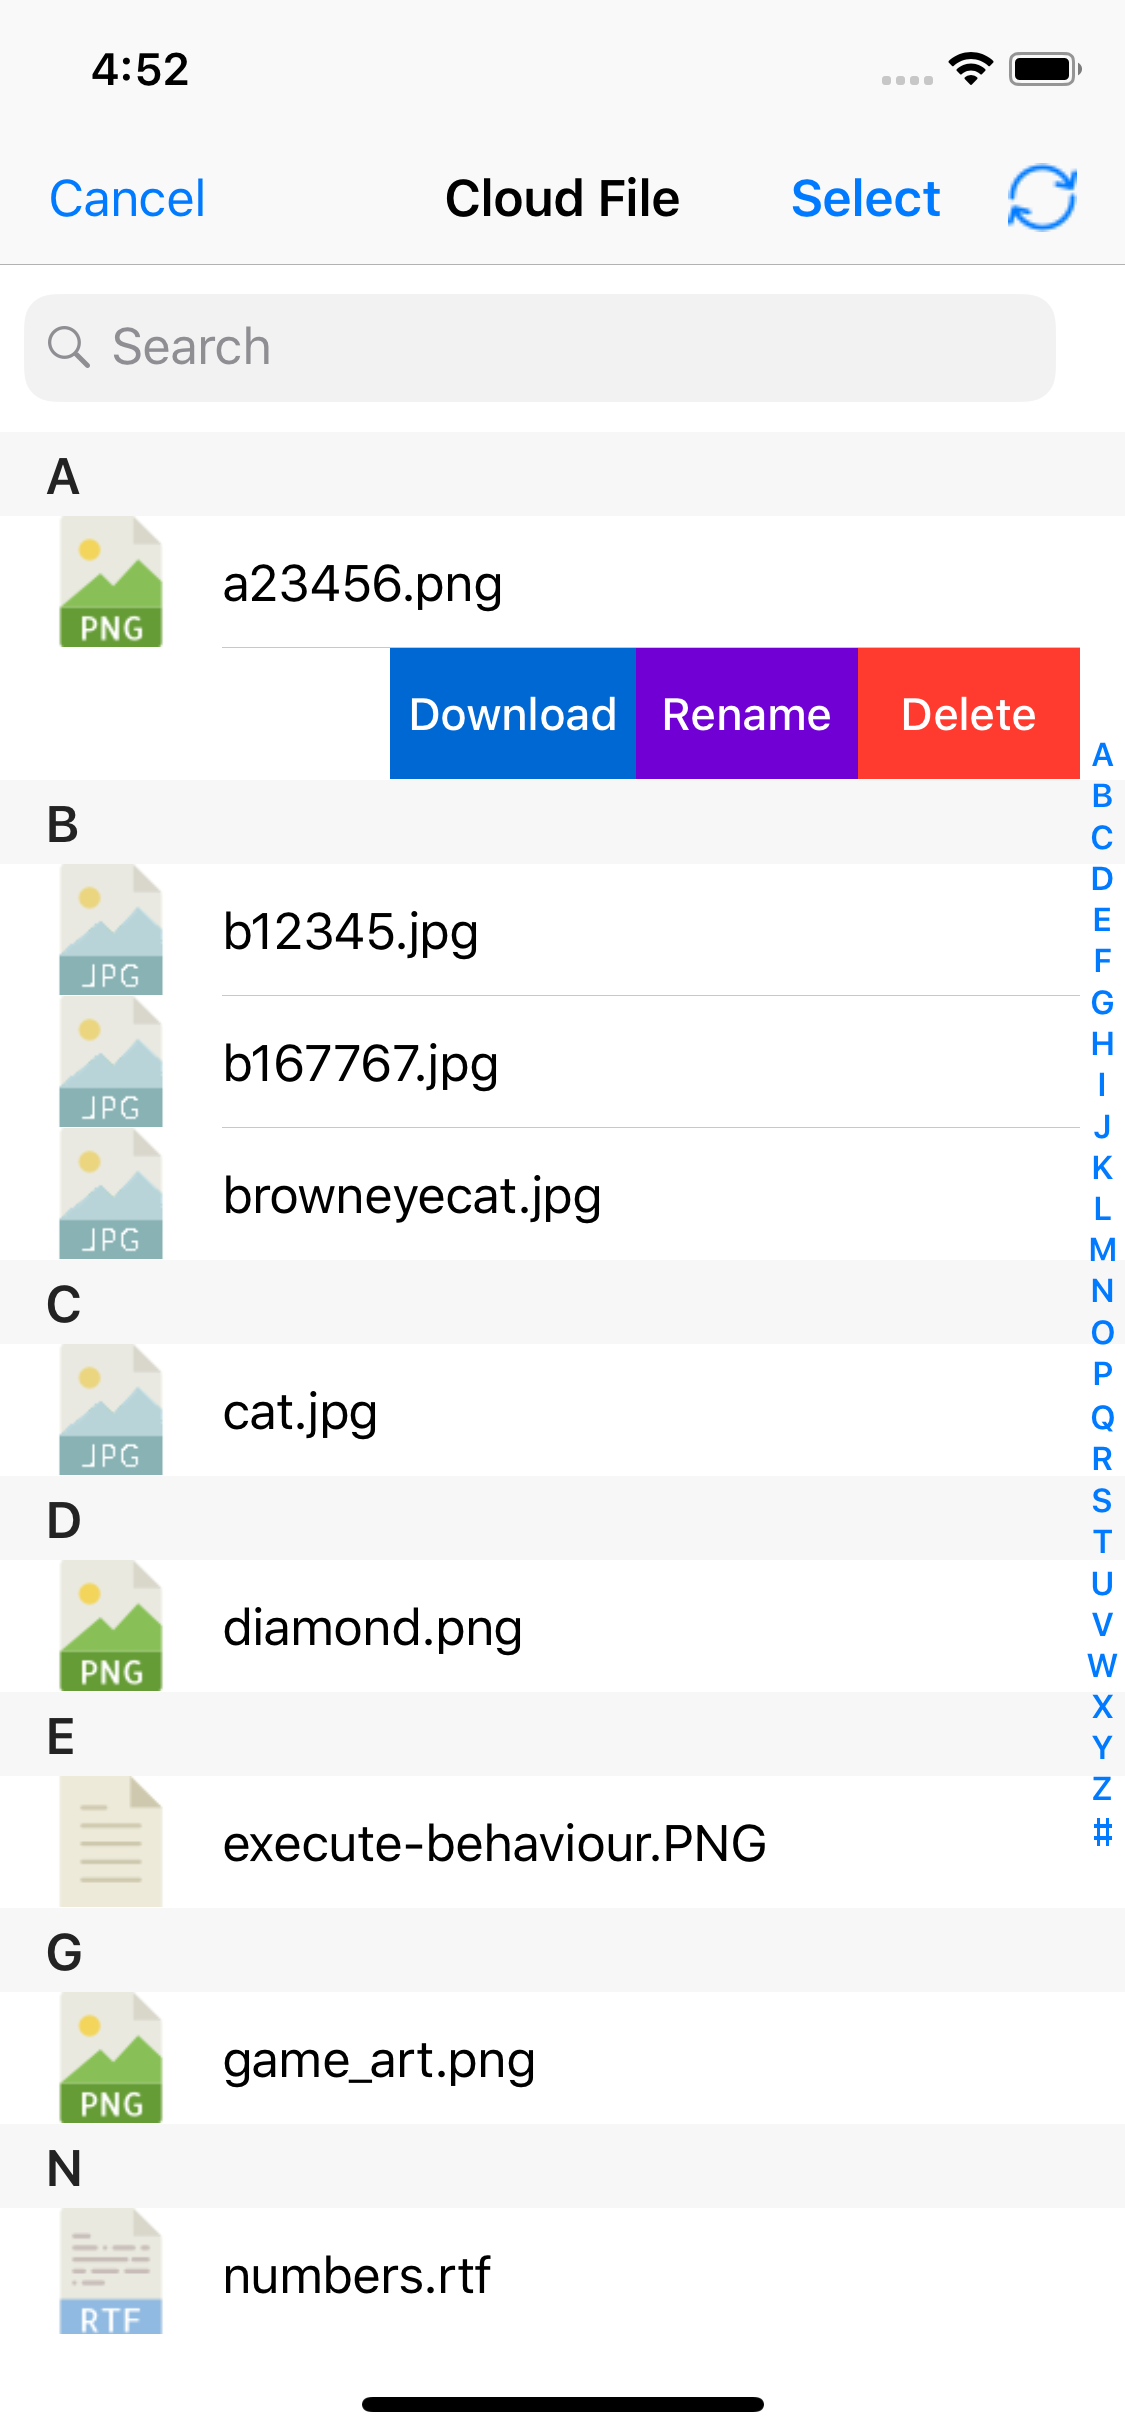
\includegraphics[width=0.19\textwidth]{24.png}\label{fig:f13}}
  \caption{TableView Functions}
\end{figure}
 
The mobile client regards to access the photo album for following the current trend. My Album page is also part of Local Files. The expectation of the users to operate a flexible and extensible application which allows them to upload and share photos opens the way for adding functions of picking up a photo in iOS album. Users can look through and check photos locally before uploading one of them to the server. Figure \ref{fig:example17} below shows the user interface of picking a photo from your iPhone.

\begin{figure}[H]
    \centering
    \subfloat[Albums]{{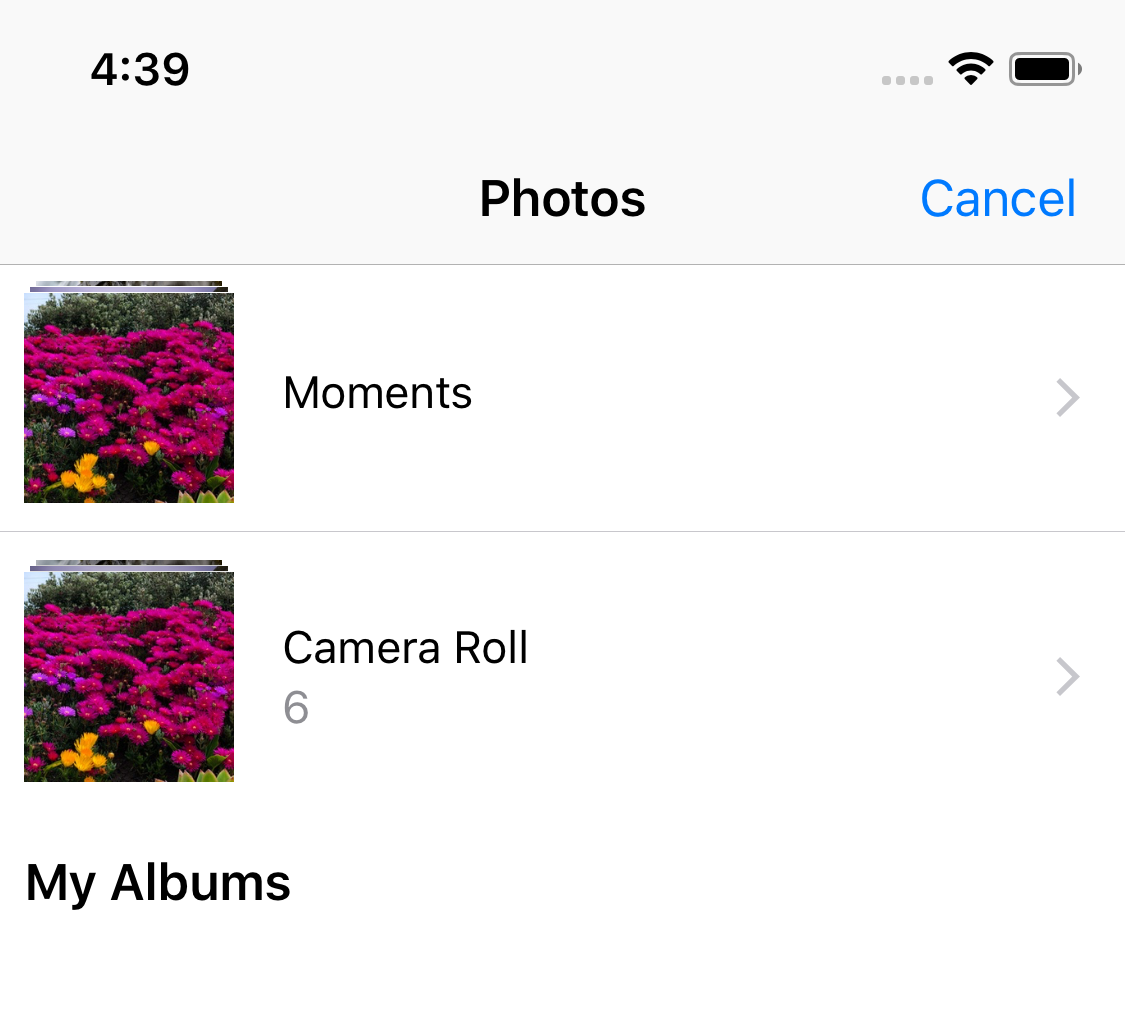
\includegraphics[width=4cm]{13.png}}}
    \qquad
    \subfloat[Selecting a photo]{{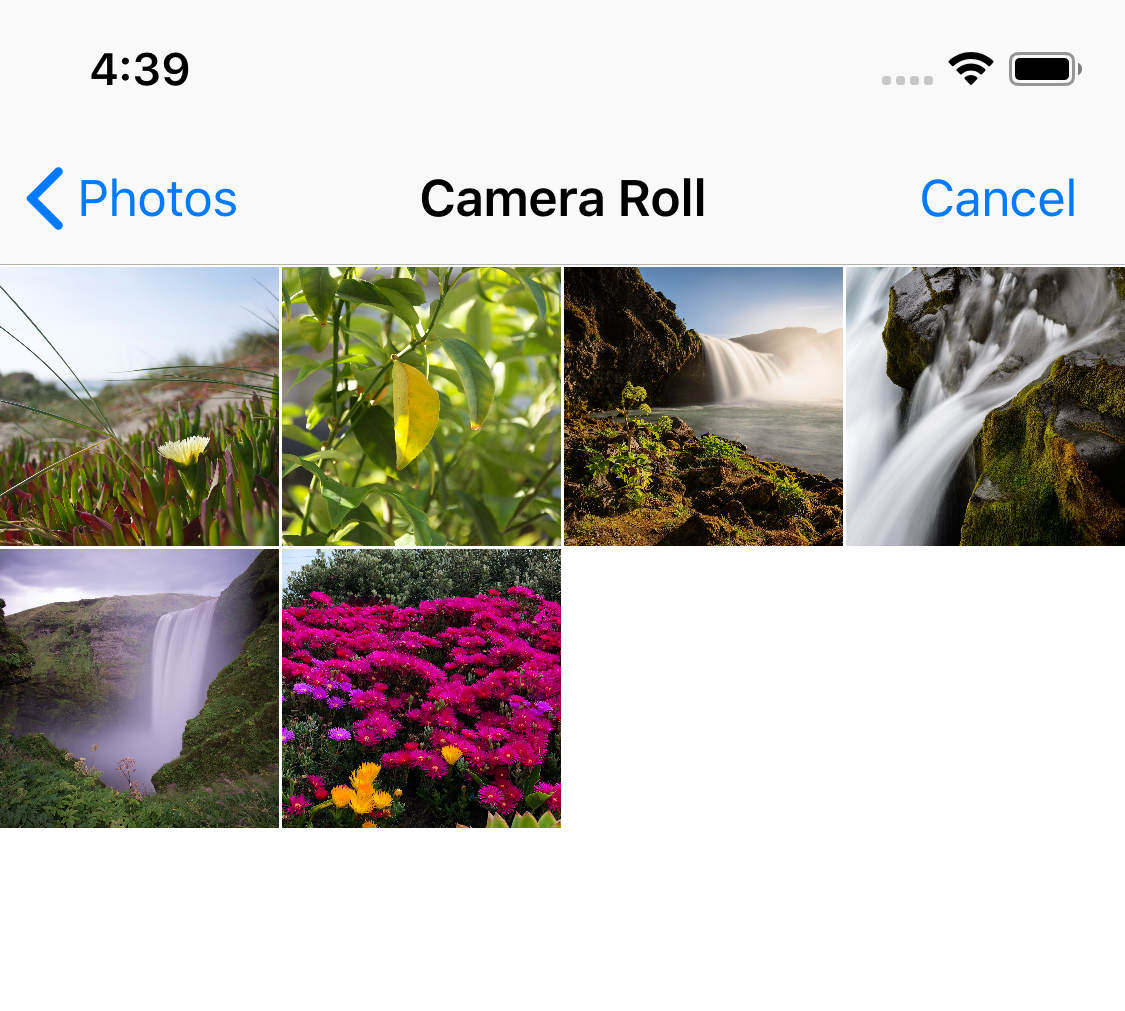
\includegraphics[width=4cm]{14.png}}}
    \caption{Photo Album}%
    \label{fig:example17}%
\end{figure}

Like Trash and Local Files, the Cloud page follows Xib design of TableView and files are listed in alphabetical order. A preview of the web page is supported for the users to have a look at the cloud files they are interested in. The mobile team will use API and HTTP to get the file data from the server (more details will bed discussed in the next section). Different icons will be used to support each file format inside the TableView. The cancel button is designed to allow the user to return to the welcome page, the select button will be for selecting specific files to download into local memory and the sync button will be for manually synchronising with the server,where all of these buttons can be found in a navigation bar. 

In the Cloud page, users are able to slide a table cell from right to left which allows them to access the rename, delete and download buttons. All of the operations shown in the Cloud page are directly connected to the server with HTTP request and the TableView will automatically update when receiving a WebSocket messages from the server. The search bar shown in the top can help the users to find a specific server file in a convenient way. The files deleted in the Cloud page will be removed permanently from the server, while the files deleted from Local Files will be move into Trash. The Trash will provide a function that can help the user to recover the files back to the Local Files. The figure shown below lists the Trash views.

\begin{figure}[H]
  \centering
  \subfloat[Trash page]{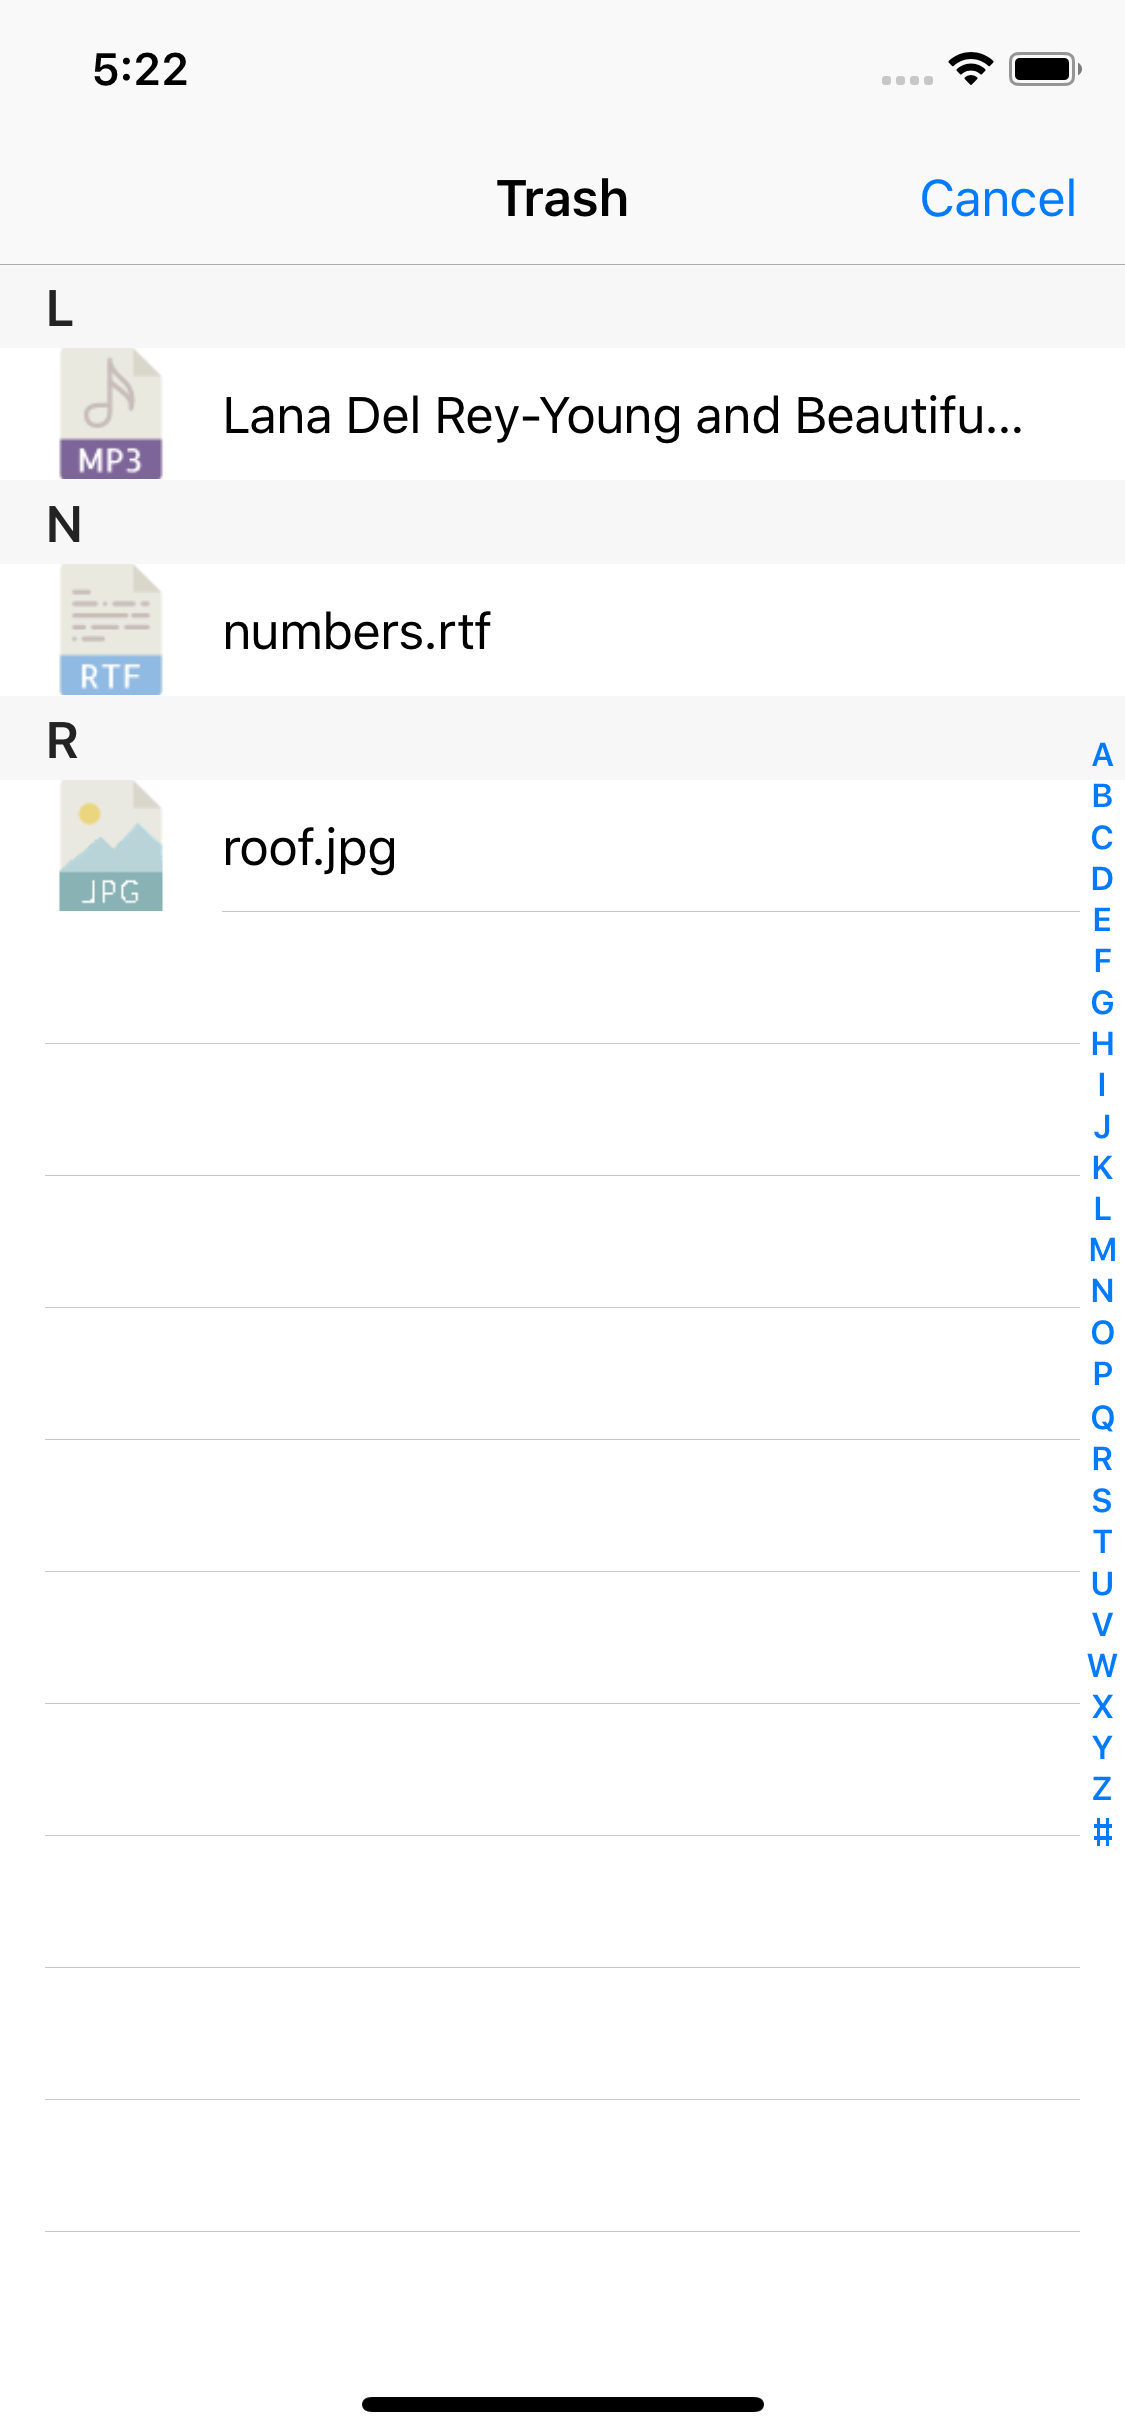
\includegraphics[width=0.19\textwidth]{25.png}\label{fig:f20}}
  \hfill
  \subfloat[Trash functions]{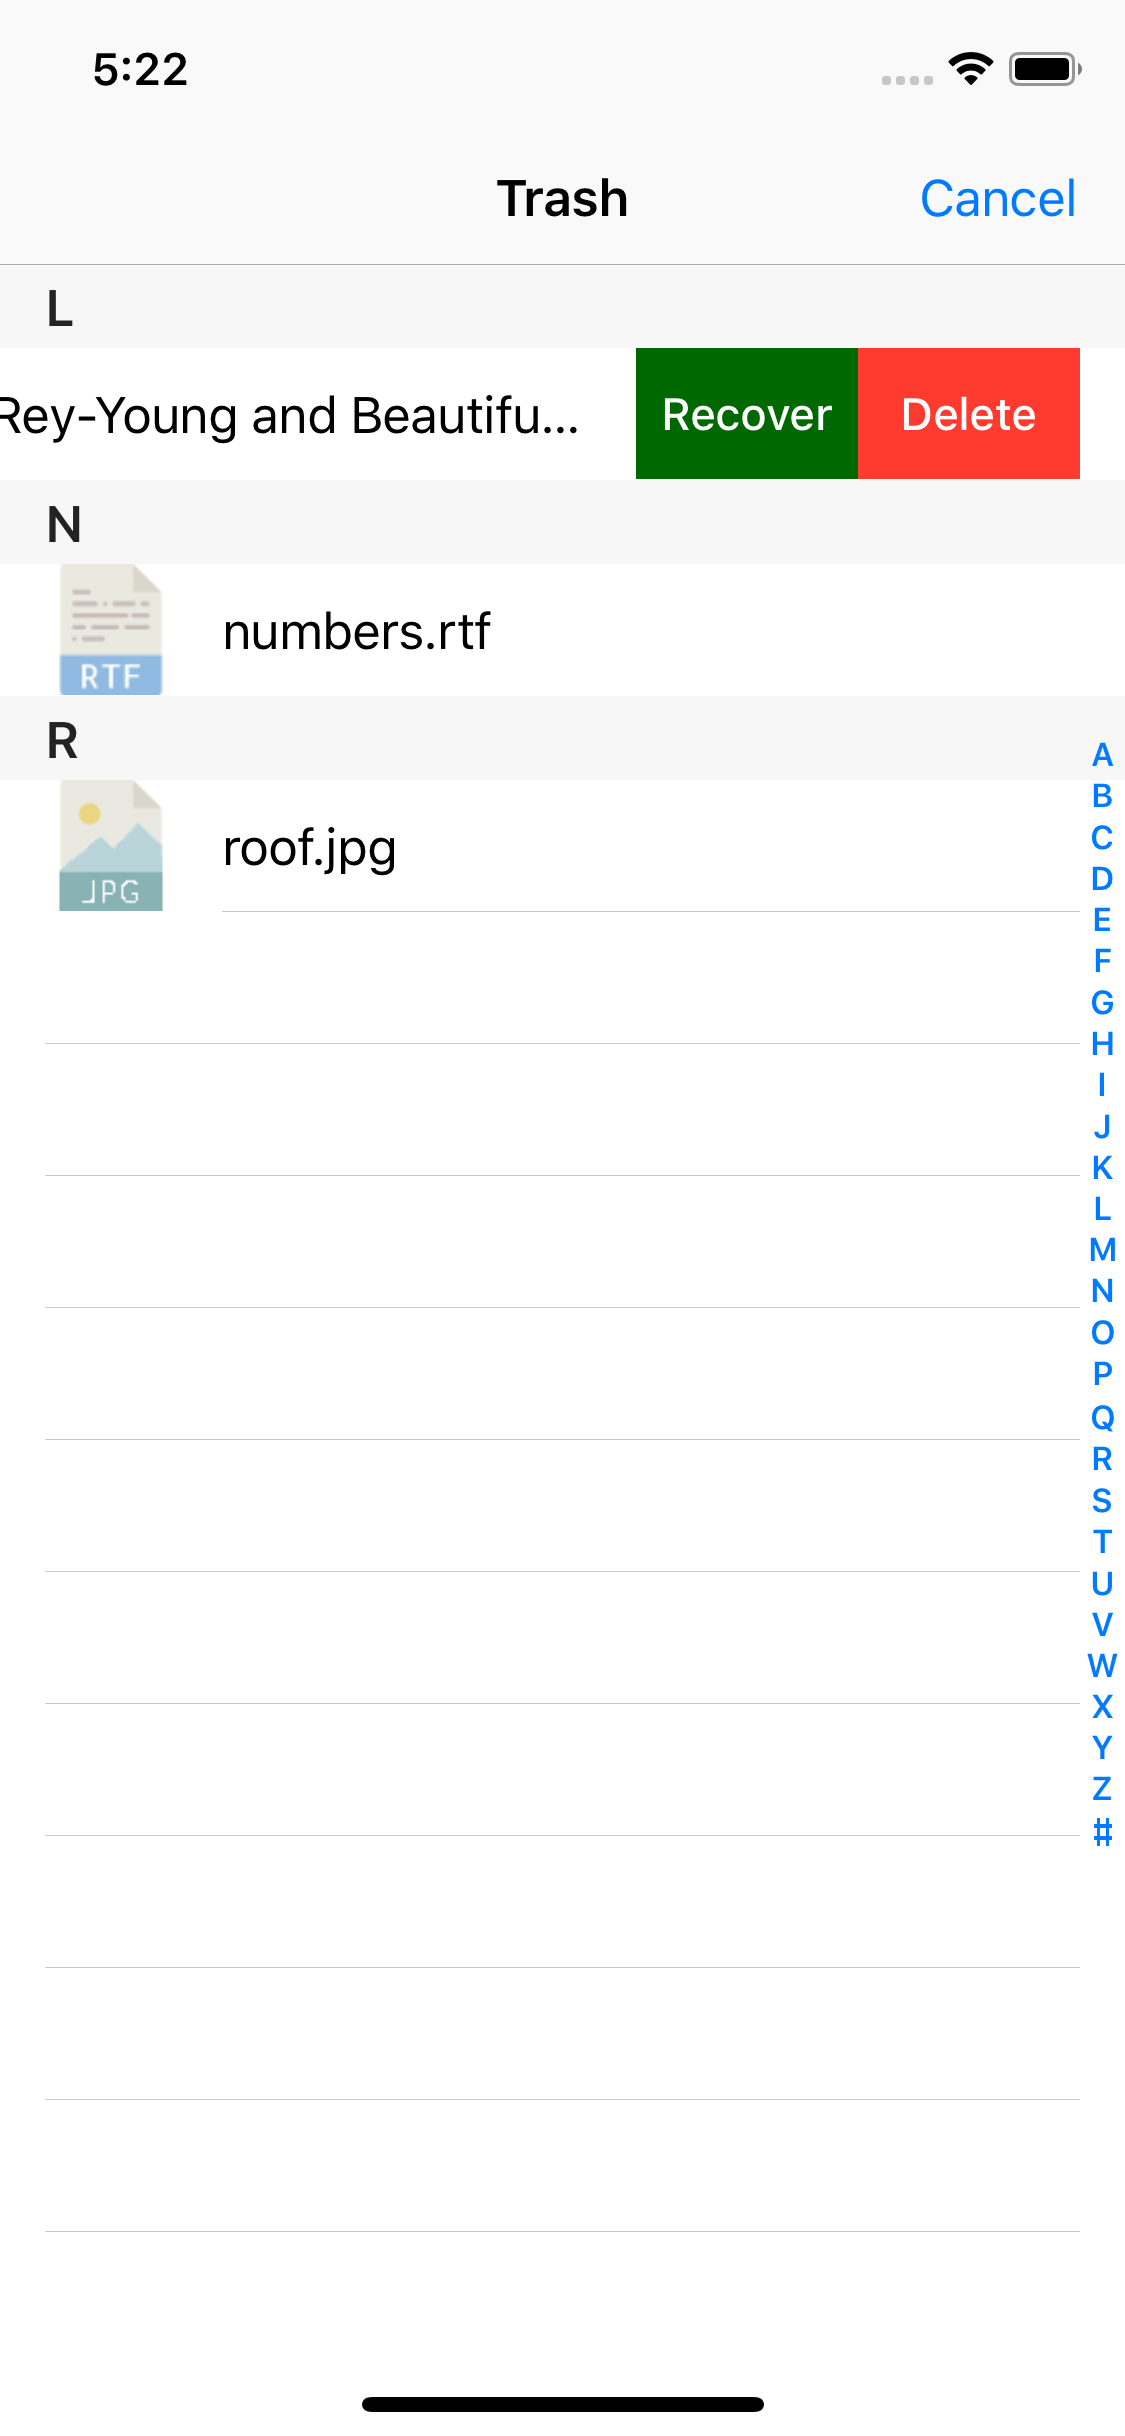
\includegraphics[width=0.19\textwidth]{26.png}\label{fig:f21}}
  \hfill
  \subfloat[After recovering]{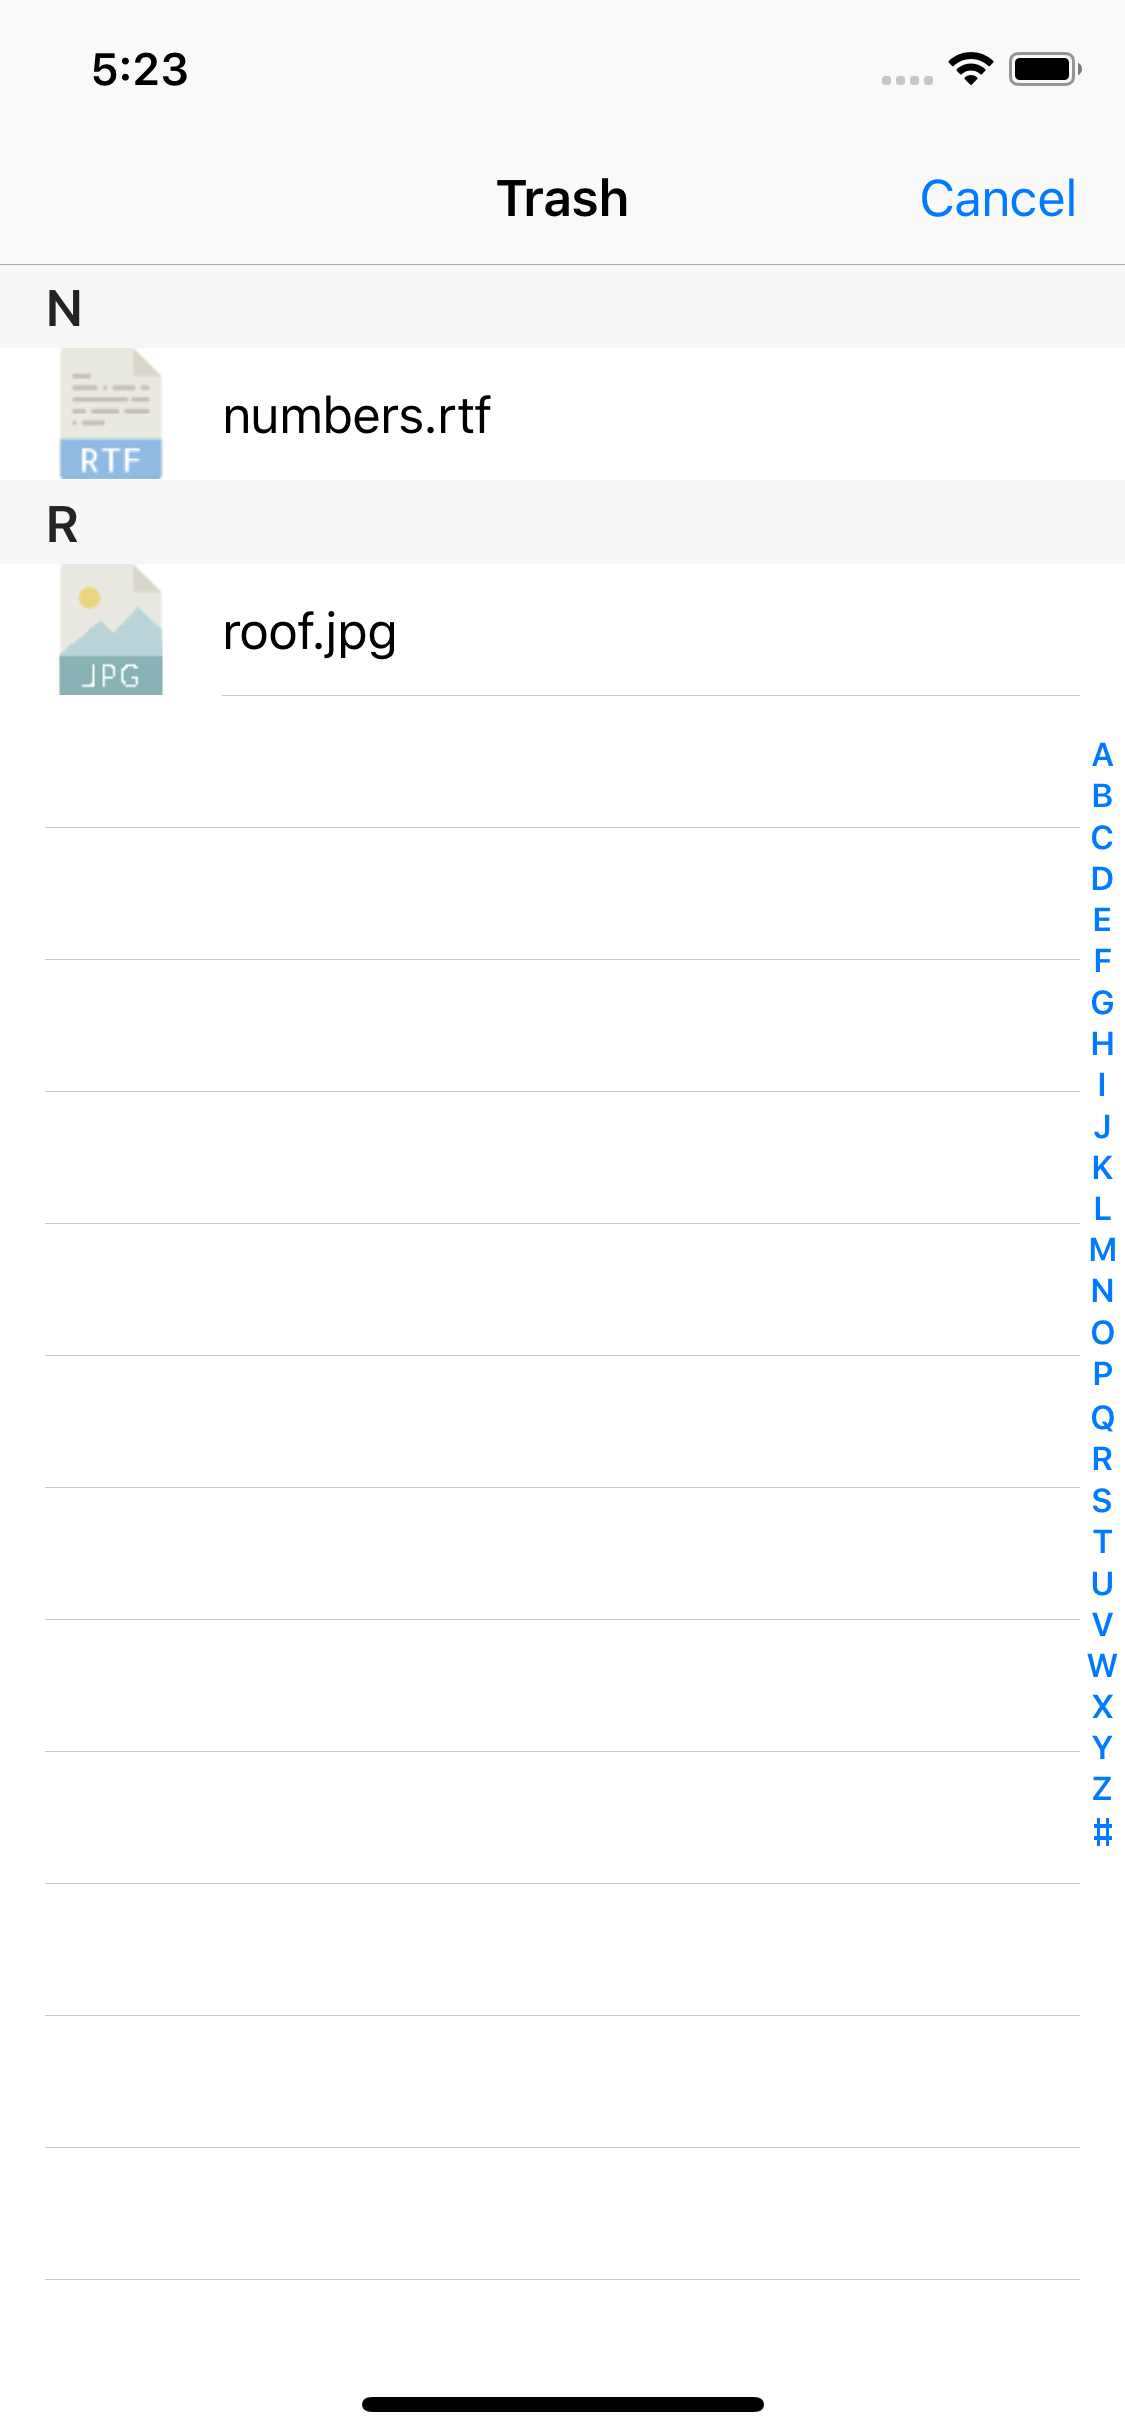
\includegraphics[width=0.19\textwidth]{28.png}\label{fig:f22}}
  \hfill
  \subfloat[Recovred files]{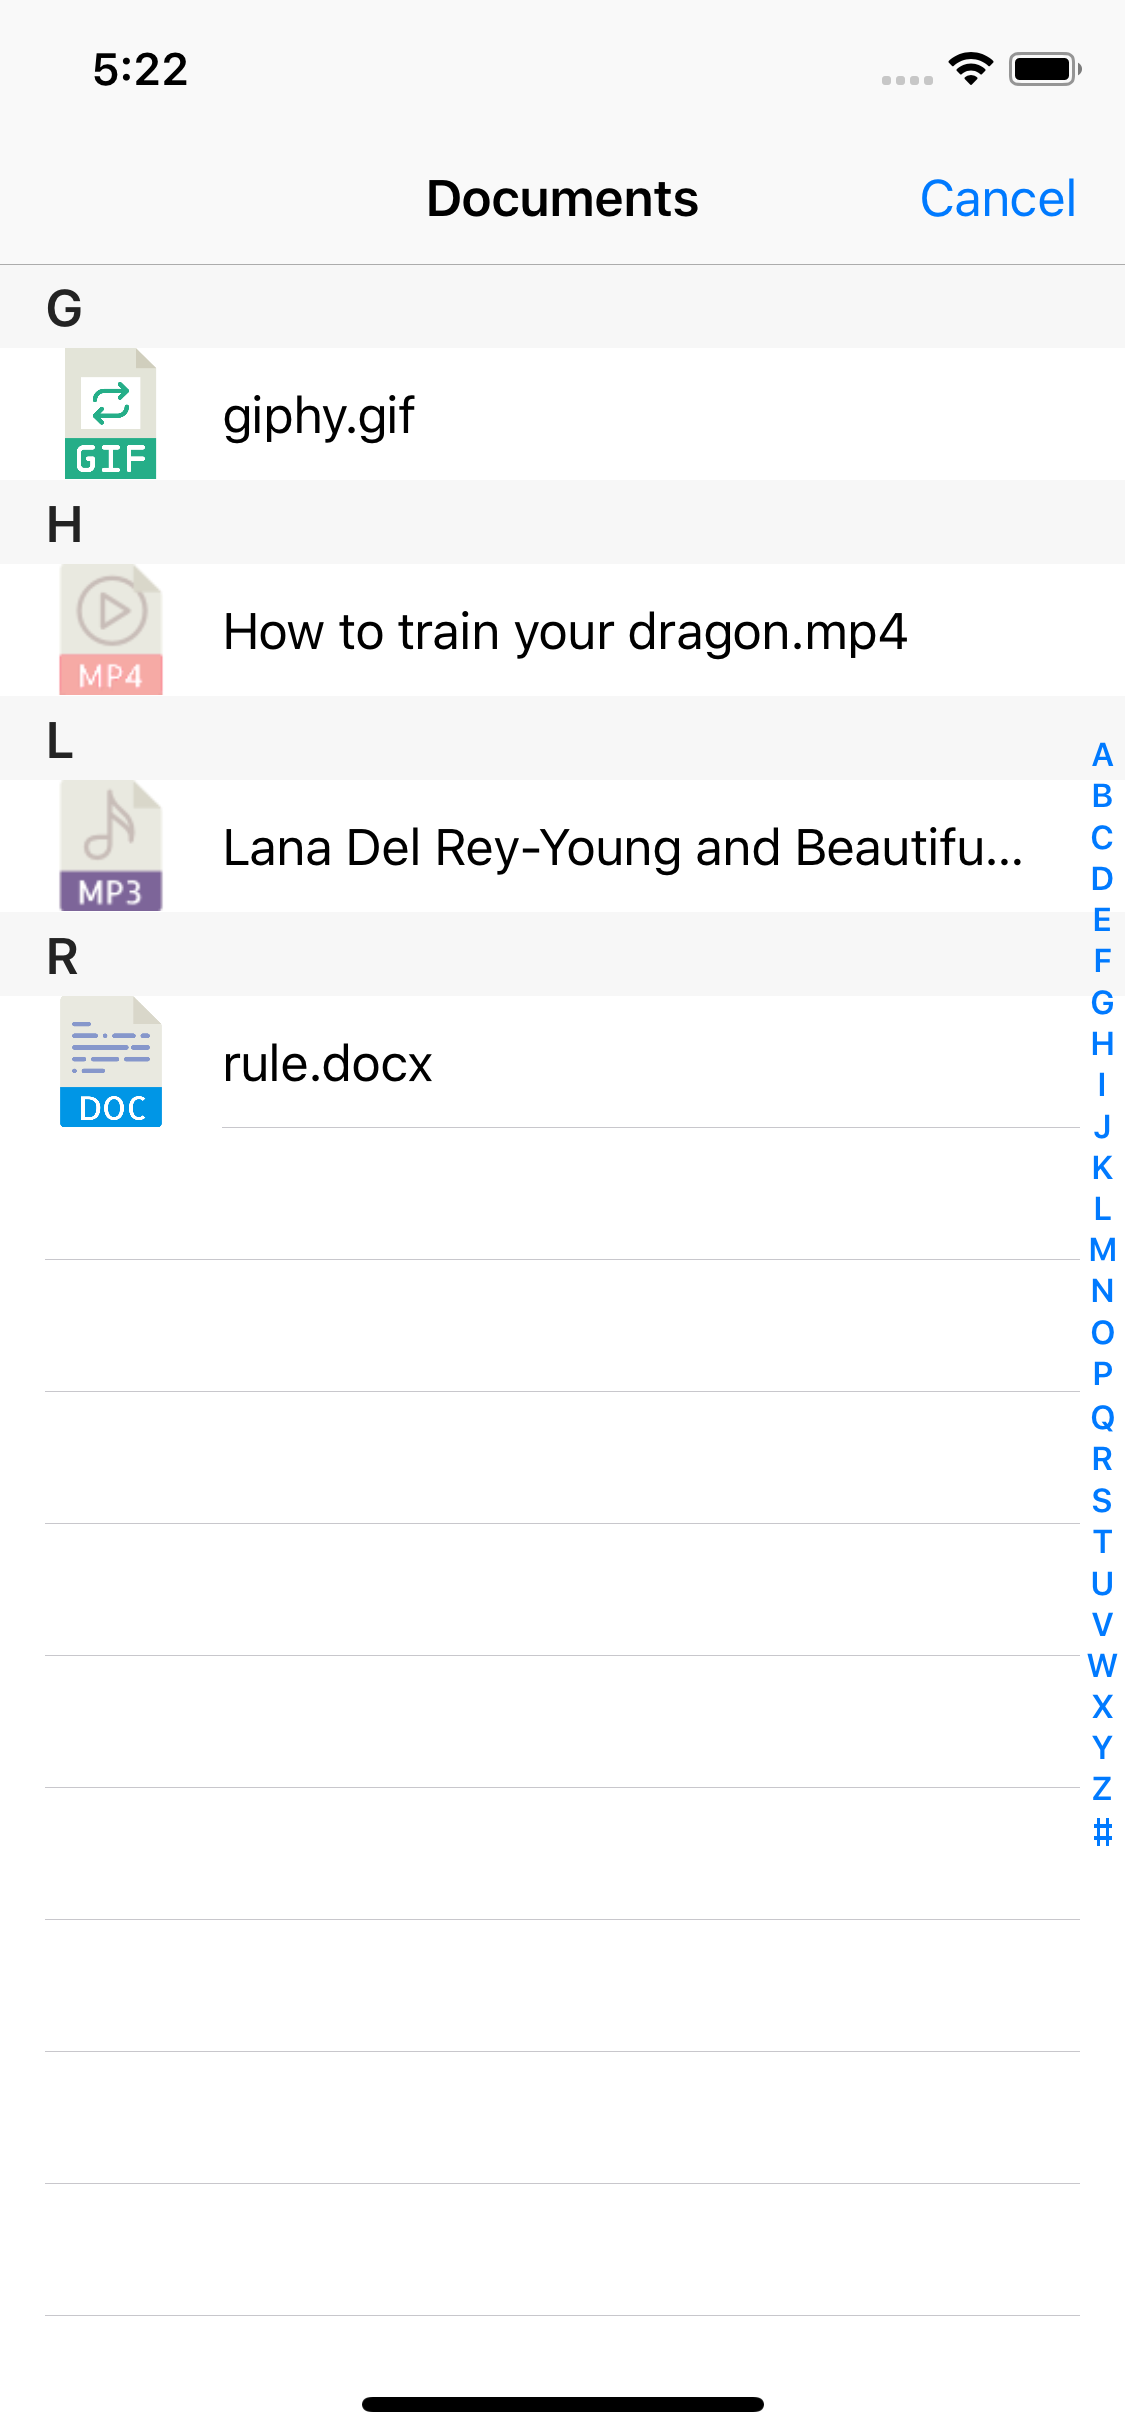
\includegraphics[width=0.19\textwidth]{27.png}\label{fig:f22}}
  \caption{TableView functions}
\end{figure}

The settings page has three table cells: App Information, Report Error and Software update menu, where it will displays the relevant information to the users.

Every page has a back button for users to return to the previous page and the navigation menu is set for users to transfer between different pages. However, the users will have to return to the main page before moving to another page. All the pages except for the custom TableView has constraints on defining the sizes of components. For example, the height and width of the navigation bar will be fixed and the navigation bar will always be kept horizontally inside the container. This allows the mobile clients to be able to run the app in every iPhone models without component compatibility problems. Finally, the Figure \ref{ex4} shown below represents the mobile application icon.
\newline
\begin{figure}[H]
\begin{center}

\includegraphics[width=3cm]{APPIcon.png}
\end{center}
\caption{Mobile Client Application Icon}\label{ex4}
\end{figure}

\subsubsection{Desktop Client}

\begin{figure}[H]
\begin{center}
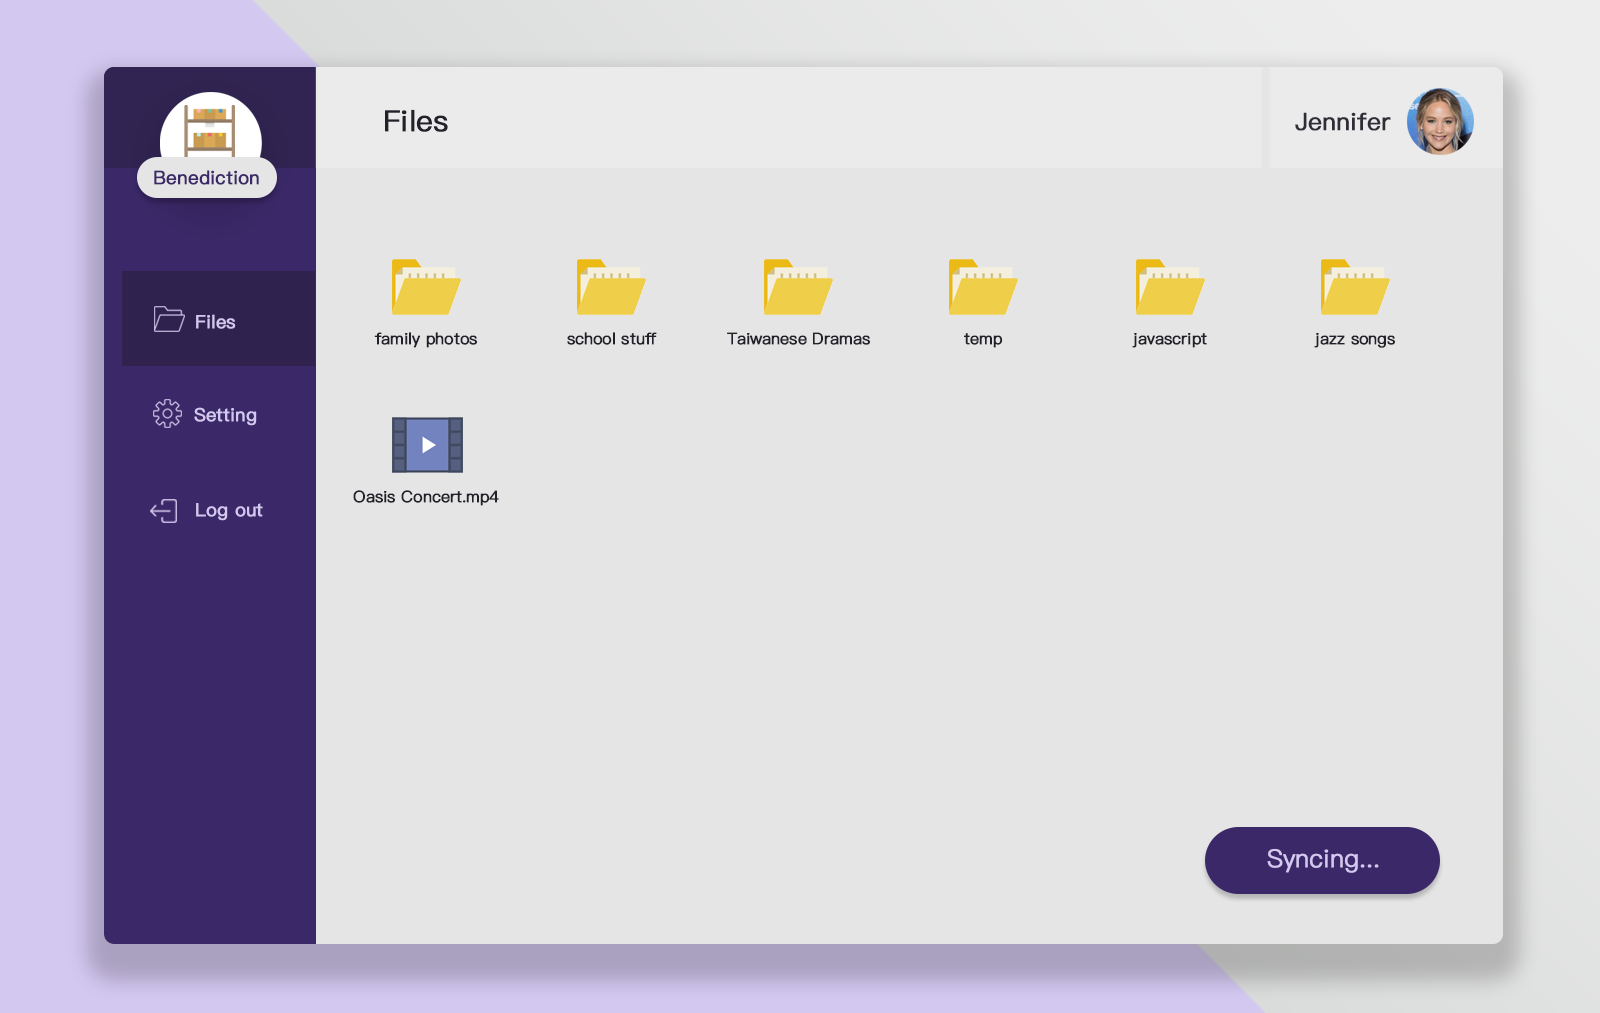
\includegraphics[width=9.5cm]{desktop-client.png}
\end{center}
\caption{Desktop client User Interface.}\label{ex4}
\end{figure}

The web application user interface has two main components. Firstly is the navigation bar on the left hand-side which allows the users to navigate through different features(pages) of the application. The team has decided to have \textbf{Files}, \textbf{Settings} and \textbf{Log out} in the navigation bar. The \textbf{Files} navigates to display the file page which contains the synchronized files from the server and allow the users to upload files on their local machine to the server. The \textbf{Settings} will take the users to the setting page which allows them to edit their personal details or find the system support. The \textbf{Log out} button is essential as mentioned above, the users will require to log in before using the system, thus naturally they will need to be able to log out of the system by using the logout button.
Secondly, the main component interface which comprises of 2 sections: the top bar and the main content container. The top bar will displays the directory and the user's profile while the main content container will displays the corresponding page the user is currently in.

To upload a file onto the server, the team will be using a drag and drop function to allow users to drag any files in their local repository into any areas of the main content container. The file would be automatically upload onto the system and would trigger the process of synchronization. The synchronized status for each file will be presented with corresponding icons, with the types of the status include uploading, downloading, synchronization failure, Up-to-date and pending to upload.

For a user to download a file, the team is inspired by the double-clicked to open file function. So instead of having a download button, the team has thought that it would be more appropriate for the user to double-click on the file they want to trigger the download function on the UI.

The front-end development will be developed in React, which is a open-source JavaScript library. This is used because it is much easier than the need to manually build user interfaces with native Web APIs and JavaScript. React also provides a component-based library which allows the team to build high-quality user-interfaces for the system web application by coding HTML and CSS inside JavaScript which makes it easier to connect the front end UI with back-end language (Node.js).

\subsubsection{File Synchronisation}

Server to client synchronisation in real time is through a FileWatcher service on the client side that monitors for any file changes on a specified application directory. The desktop application used \emph{./benedictionFiles} as the local client synchronisation folder for every user that will be monitored and files synced with those of the server. Any changes done by the user in this folder will automatically be synced with the server. If a user wants a file stored and accessed by other clients on the server, they can copy or drop it into the sync folder and it will automatically be available on the server. The same process is applied for deleting a file in the sync folder – it will also be deleted from the server. Making local changes to files in this folder will also trigger the synchronisation to the server. However, to be able to save these changes, the local file version is checked with the server file version and changes are permitted only when the versions match. Otherwise, the user will have to download the current version from the server and makes changes to that before saving to the server.

\begin{figure}[H]
\begin{center}
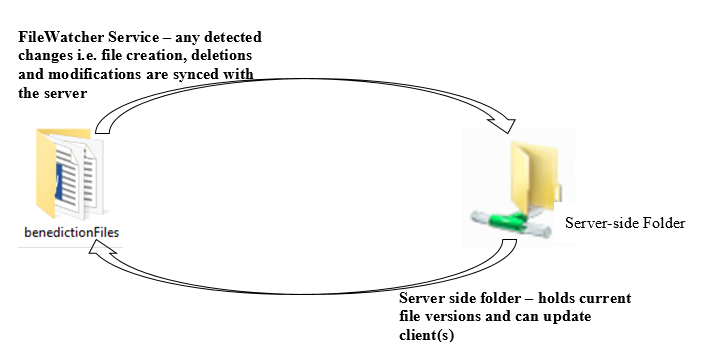
\includegraphics[width=15cm]{fileSync.PNG}
\end{center}
\caption{Client-Server File Synchronisation}\label{ex4}
\end{figure}

To enable successfully synchronisation, DirectoryWatcher service \cite{c14} was used to provide monitoring events such as new file added, file deleted and file changed to the local folder. However, the events were extended to provide functionality that would help synchronise local files with the server as can be seen below for an event when a new file is added to the local sync folder.

\begin{figure}[H]
\begin{center}
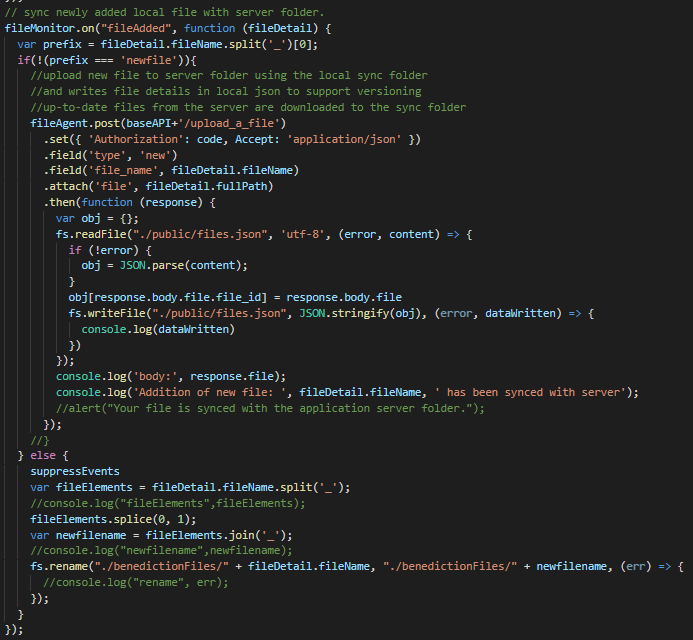
\includegraphics[width=15cm]{fileAdded.PNG}
\end{center}
\caption{Local sync folder 'file added' Synchronisation trigger}\label{ex4}
\end{figure}

The snippet shows that when a file is added it's checked for a prefix new file; if prefixed, then the file has been downloaded from the application server and is not a new file. No synchronisation is required if the file has the above prefix as it has been downloaded straight from the server, however, the prefix is removed. 
If it is indeed a new file, an API call is made to upload it to the server as well as store its version received as a response back from the server in a JSON file. The file details in the JSON file help support when a user is updating a file on the server. The file version in the JSON file is checked against the server before the update process. Only files with similar versions can be modified, and this can be from other users updating the same file previously. 


\subsubsection{Back-end Server Application}
\item\textbf{Overview}

The back-end server application is responsible for handling every business logic, file storage, database connection for this project. For serving different types of clients, the endpoints of the server application should be able to used by different sources including mobile application and desktop application. To achieve the goal, the team decides to follow disciplines of Restful API.

The team-working plays a huge role in the technical stacks. At first, two members assigned to work on the back-end application could not reach an agreement on which language to use. One of the members is more familiar with Java but the other member has no experience with it at all and more familiar to JavaScript/Nodejs. After several discussions in the team as well as initial review midway through development, the team came with a consensus of switching roles and change the language to JavaScript considering the factors described below. 

First, JavaScript is a language that works both on the client side on web development and back-end side with Nodejs, so the team members for desktop client and back-end can share their experiences, fix errors on syntax, and help each other. On top of that, JavaScript is well known to most of the group members. Most importantly, one of the members in the team has three years of industrial experience on JavaScript development. 

Overall, the team uses JavaScript and Nodejs as its main language on the back-end side as well as MongoDB and JSON as a solution for data storage. For the file storage, the server stores the files in a folder within the application. More details of the implementation and difficulties met are described below.
\newline
\item\textbf{Architecture}\newline

\begin{figure}[H]
\begin{center}
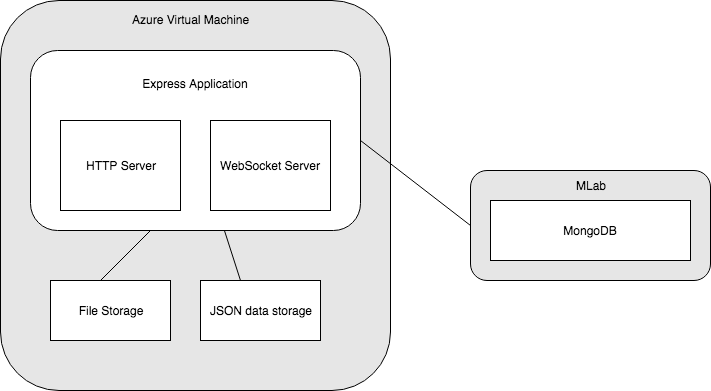
\includegraphics[width=9.5cm]{Backend_Diagram_Archietecture.png}
\end{center}
\caption{Architecture Diagram for Back-end Application}\label{ex4}
\end{figure}

The team uses Express.js as its main framework for back-end application. Express is a back-end framework based on Nodejs. the team chose Express for multiple reasons such as its simplicity, which means that each function can choose any components to build. Although each function has its own scaffolding, it will take less time to build an integrated basic framework.

Additionally, other advantages such as flexibility, a vast number of plug-ins, free to use and frugal, and its suitability for simple business logic models.  Express mainly adds routing, middleware and template mechanism on the basis of HTTP library, which provides basic tools for rapid development.
\begin{figure}[H]
\begin{center}
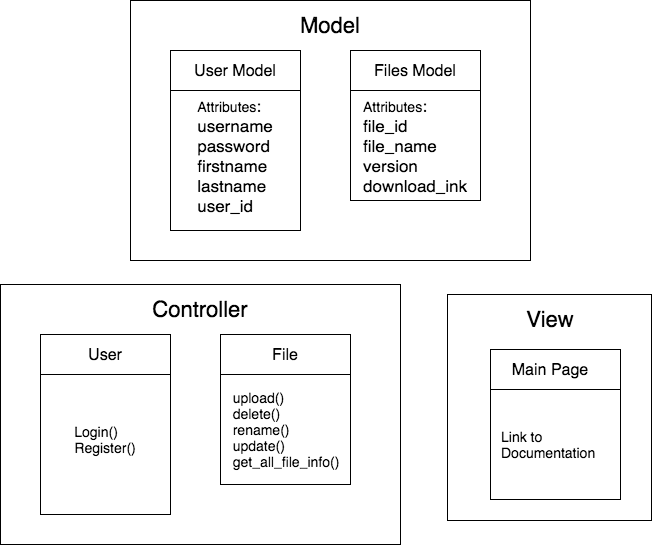
\includegraphics[width=9.5cm]{Backend_Diagram_MVC.png}
\end{center}
\caption{Back-end Diagram for MVC Model}\label{ex4}
\end{figure}
The team also applies an MVC model to implement the application. The Model-View-Controller (MVC)  is an established architectural design pattern for developing interactive, object-oriented applications. It is an architectural pattern that separates an application into three main logical components: the model, the view, and the controller. Each of these components is built to handle specific development aspects of an application.\cite{c6}

The controllers are the components to deal with business logic. In this project, the team divided the controller functions into two separate controllers. The first controller is designed to handle all the requests related to file operations such as uploading, downloading, renaming, updating and deleting a file on the server, named as \emph{fileRouter.js} in the project. The second controller, \emph{userRouter.js} is designed to handle all requests related to users and authorization such as logging in and user registration. 

The views of the project on the back-end application are not the views on the client side. In other words, in the basic requirements, the back-end team created a page that includes the documentation of the endpoints in order to let other developers have easy access to the developed endpoints.  

The model parts of the application are designed to specify the structure of the data stored and to offer encapsulated modules for other parts of the project to directly access the database. This also avoids redundancy of code for functions that deal with database connections.

\newline
\textbf{Documentation}

The team also made documentation describing all the details for endpoints in the back-end application. The document is hosted in Google Drive platform in a format of Google Doc file. The document consists of three parts. First, an overview of the mechanism of the connection between client and server is described including authorization, logging in/out, and the difference between HTTP connection and WebSocket connection. The second part of the documentation is to offer information for all the HTTP endpoints with details including URL, description, fields in the request body, and the structure of the response. In the last part of the documentation, the team listed all the WebSocket events that should be listened to by the clients as long as its details include event names and their payload.

\newpage
\section{Implementation}
\subsection{Mobile Client}
\subsubsection{Login/Register Authentication}

The Login/Register authentication in mobile client includes register, log-in, log out functions. The mobile client set the GlobalToken as a String variable (in Httphelplers.swift), which can be used on every page where GlobalToken is a returned value sent by severing after a user logging into system successfully. Users must log in before they visit the Cloud page. Since the mobile client will check the length of GlobalToken before giving user' permission to visit Cloud page. In order to login/register, the mobile client uses HTTP.request.post with the help of the SwiftHttp library \cite{c11}. The username and password will also be stored locally as a global structure and the profile (which is used for showing user information) can have access to it.

\subsubsection{TableView Controller and App Data Delegate}
A custom TableView is applied to the mobile client following the design of a library \cite{c10}. As mentioned above, Cloud page, Trash and Local Files all obey this fundamental user interface design. Delegate and data source are set in Xib files. In order to get the precise location of each file in this TableView, a two-dimensional vector is created in each TableView. It records the location of the file since the NSIndexPath (provided by UIKit) contains two parameters: section and index. Then for confirming file's location, both of section and index are required to draw a request (after searching a file, only one parameter index is needed because the section is already confirmed). 

The data source of the Cloud page is connected to the App Delegate. The system aims for achieving synchronization automatically and Websocket acts as a bridge between client and server. As long as there are any changes of files happening in the server, the mobile client will receive the message. However, the connection is not stable and app delegate has to ensure the connection by using websocketdelegegate and socket.connect(). Those functions monitor the connection status and will connect to the server immediately once they detect any disconnection signal. 

\begin{figure}[H]
\begin{center}
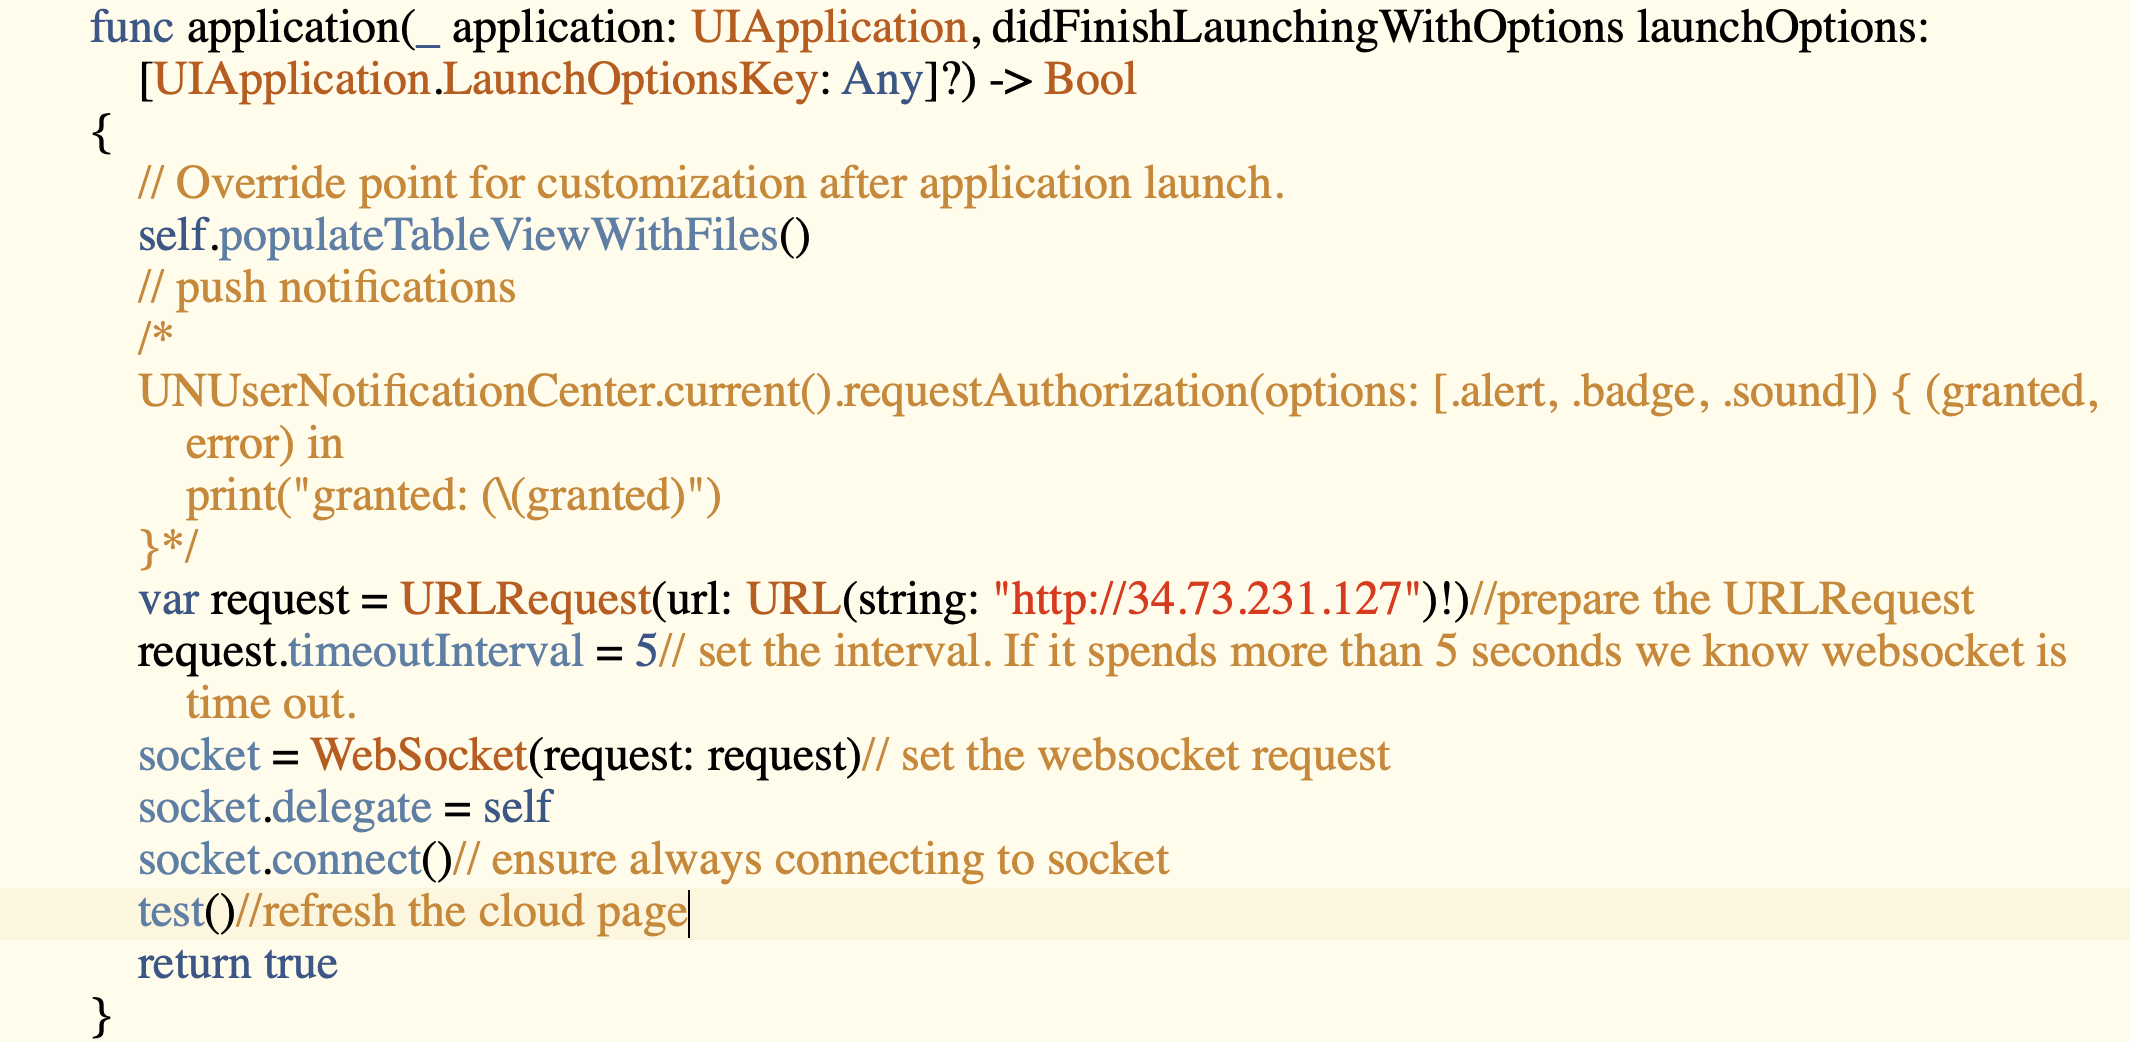
\includegraphics[width=12cm]{29.png}
\end{center}
\caption{Cloud page data source}\label{ex4}
\end{figure}

The file information got from the server and the local file list are all public NSObject classes. Another class named 'TranslateFiles.swift' is created and used as a class list to represent various types of files. All the files in TableView can be viewed by users, although some formats are not supported (like wmv and avi). For providing the preview of files, a framework named quick player is applied and all the three classes (Trash, Cloud and Local Files) are extended with 'UIViewControllerPreviewingDelegate'. The previewingContext gets the location of files in the table view through the index path and calls the related function to show the file contents.

\subsubsection{HTTP Request and WebSocket}

This section supports the mobile client to achieve file synchronization. The SwiftHttp \cite{c11} and a websocket library \cite{c12}) are used for maintaining the connection to the server and sending the request messages. Public structures and classes are created for decoding the JSON response sent from the server. The mobile client has to use a public structure for saving cloud files information because the URL session (used for HTTP request) is an asynchronous function that doesn't support assigning values to local variables. There is a small difference between downloading and other requests. Since downloading makes use of files' URL address (which also need an HTTP header), in this step, there is no need for HTTP POST/GET. Figure \ref{fig:f24} and \ref{fig:f25} are code snippets of HTTP handlers.

\begin{figure}[H]
  \centering
  \subfloat[Download Request]{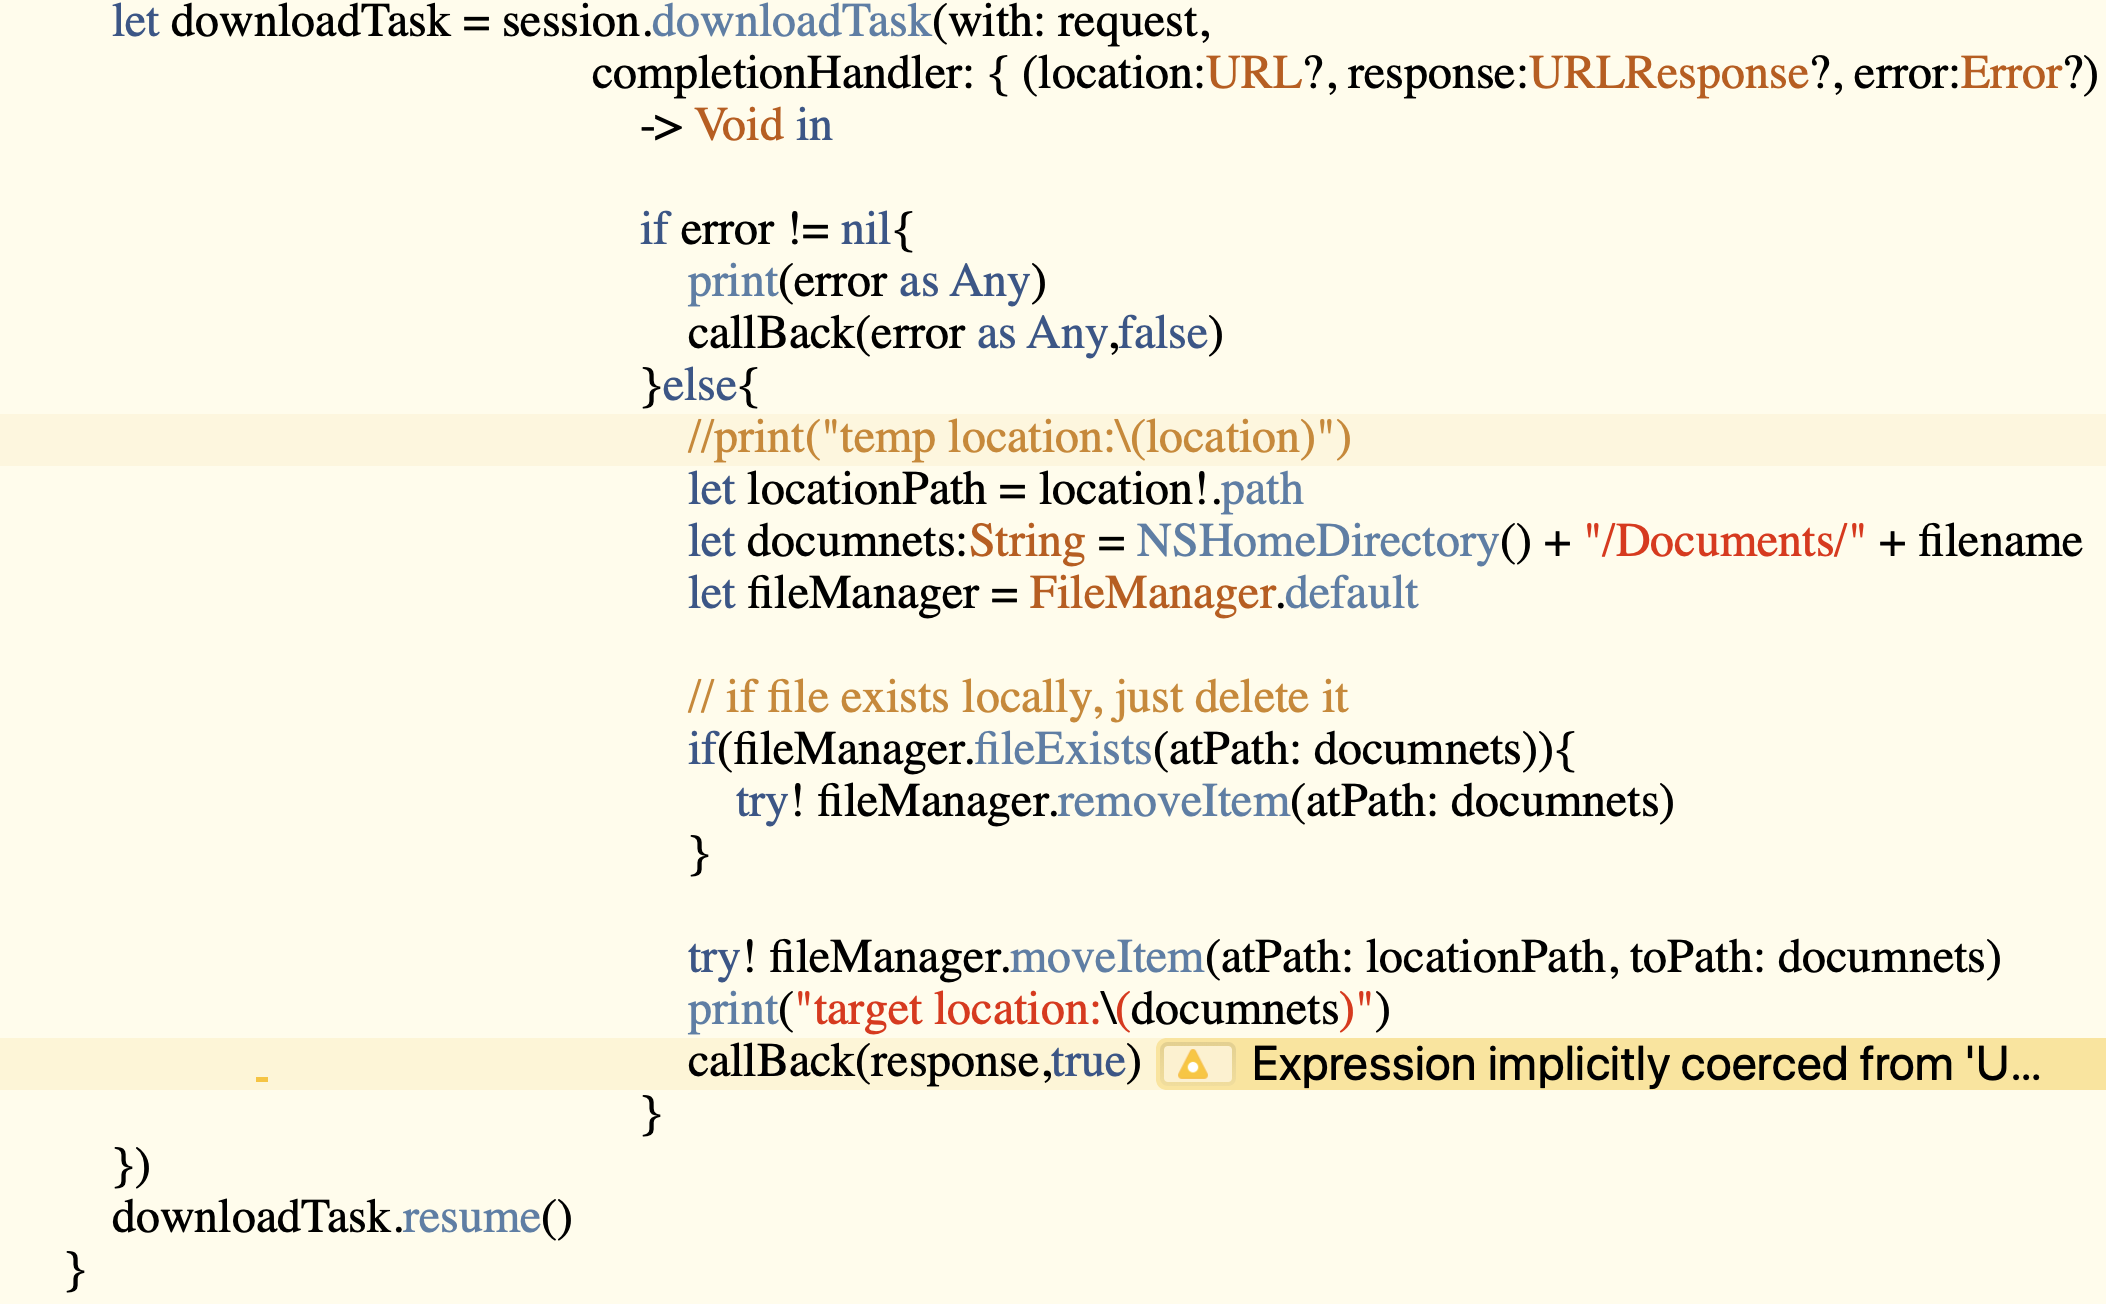
\includegraphics[width=0.49\textwidth]{30.png}\label{fig:f24}}
  \hfill
  \subfloat[Upload Request]{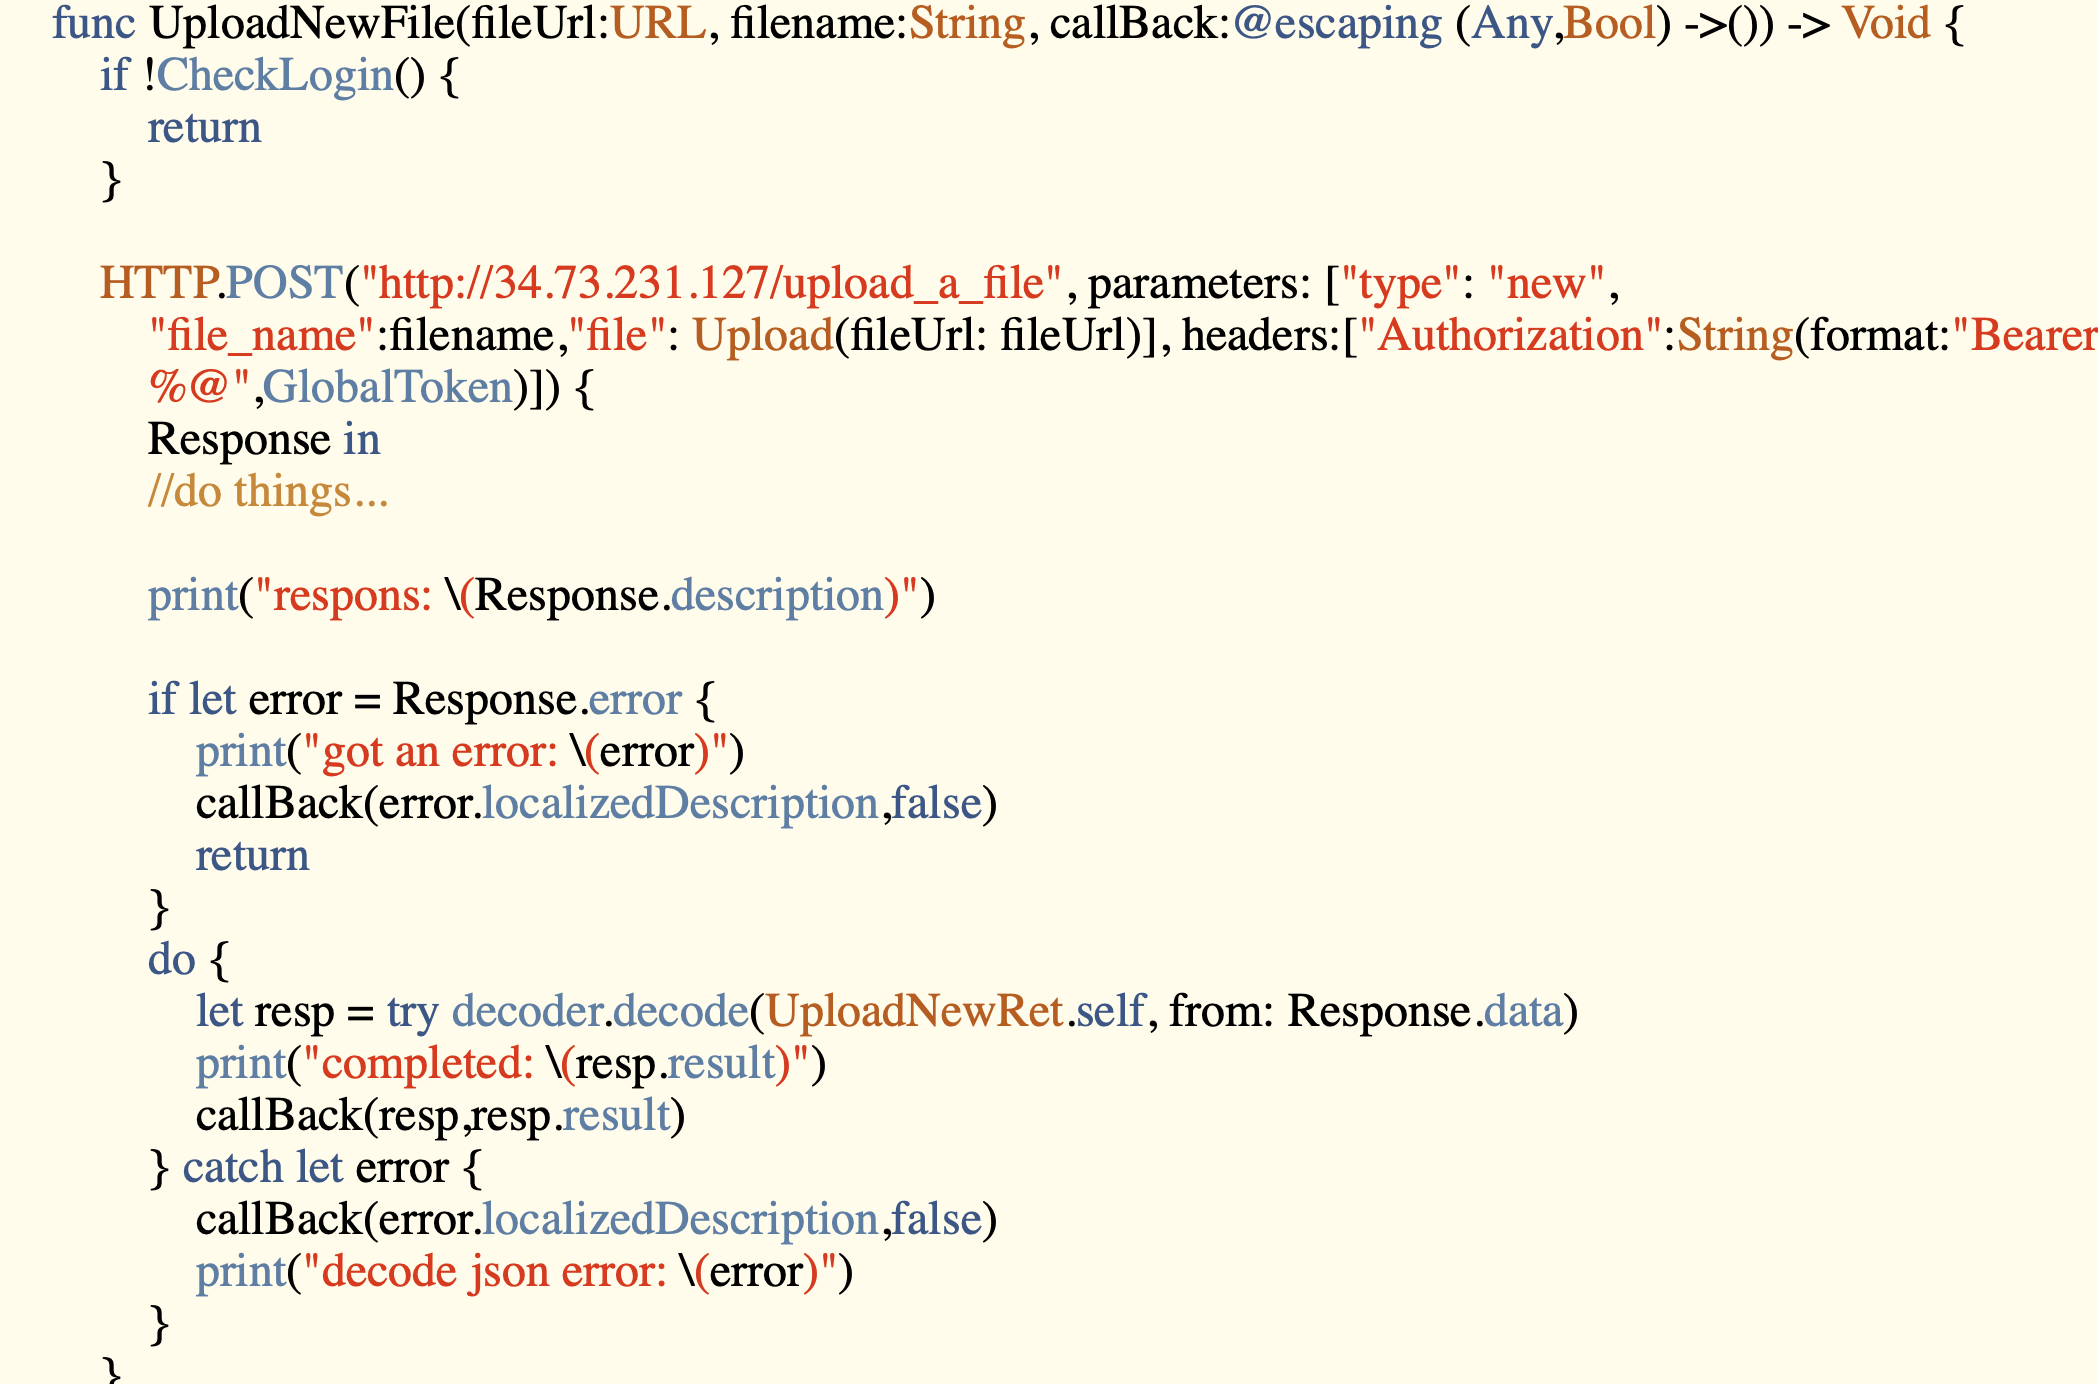
\includegraphics[width=0.46\textwidth]{31.png}\label{fig:f25}}
  \caption{HTTP handlers}
\end{figure}

WebSocket allows the mobile client to keep in touch with the server and have real-time updates. The delegate of WebSocket is applied as a combination of functions which are responsible for checking the WebSocket status and returning the information of received data and messages (shown in Figure \ref{ex011}). HTTP handler acts as a public class that provides uploading, renaming, downloading, deleting, getting files information, logging in and registering. An extension of UIWindow is used for specifying the current view controller. 

\begin{figure}[H]
\begin{center}
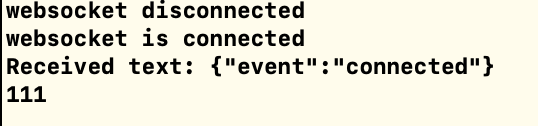
\includegraphics[width=9cm]{36.png}
\end{center}
\caption{Monitoring messages of WebSocket status in console}\label{ex011}
\end{figure}

The mobile client address the issue of solving conflicts in this part. For example, when a cloud file is renaming by a user in a mobile client, and this file is deleted from the iCloud in another client. After the user finishes rename and upload request, there will be a conflict. With the aim of solving this problem, a Boolean variable is set for checking if a conflict exists. When this Boolean variable is false, then the rename of that could file will be forbidden locally. The downloading request sent by HTTP in the mobile client will always fetch the newest version that is saved in the server and all the files downloaded from the server can be found in Local Files. 

\subsubsection{Foundamental Operations}

The TableView provides an icon matching for each type of files. All the files are recognised in the same way. First, an enumeration is created to save all the formats' name (like mp3, mp4 and so on). Then the file's extension is cut from String lists and saved as a class type. The TableView also has five main functions, which are responsible for renaming, uploading, downloading, deleting and recovering a file. The situations are different with respect to different Swift view controllers. The download function of Cloud page combines HTTP request and table cell selection. Files that have been downloaded are saved via a local folder string (NSHomeDirectory() plus the folder name). Deleting a file in the server will call the API and send a request to the server. Deleting a file locally means that we transfer a file from local files to Trash. FileManager.Default.moveItem(atPath:toPath:) is used in this step. FileManager is an interface provided by Apple, which helps developers to interact with the file system. Deleting a file in Trash or in Cloud means that this file has been removed permanently. 

The HTTP API of server actually provides six kinds of fundamental operations. The function of getting files information from the server is performed in two ways. One of them stands for automatically updating the Cloud TableView, and another is related to the synchronization button shown in the navigation bar. The former one depends on both HTTP request and WebSocket messages. The latter one only has interaction with HTTP API. 

\begin{figure}[H]
\begin{center}
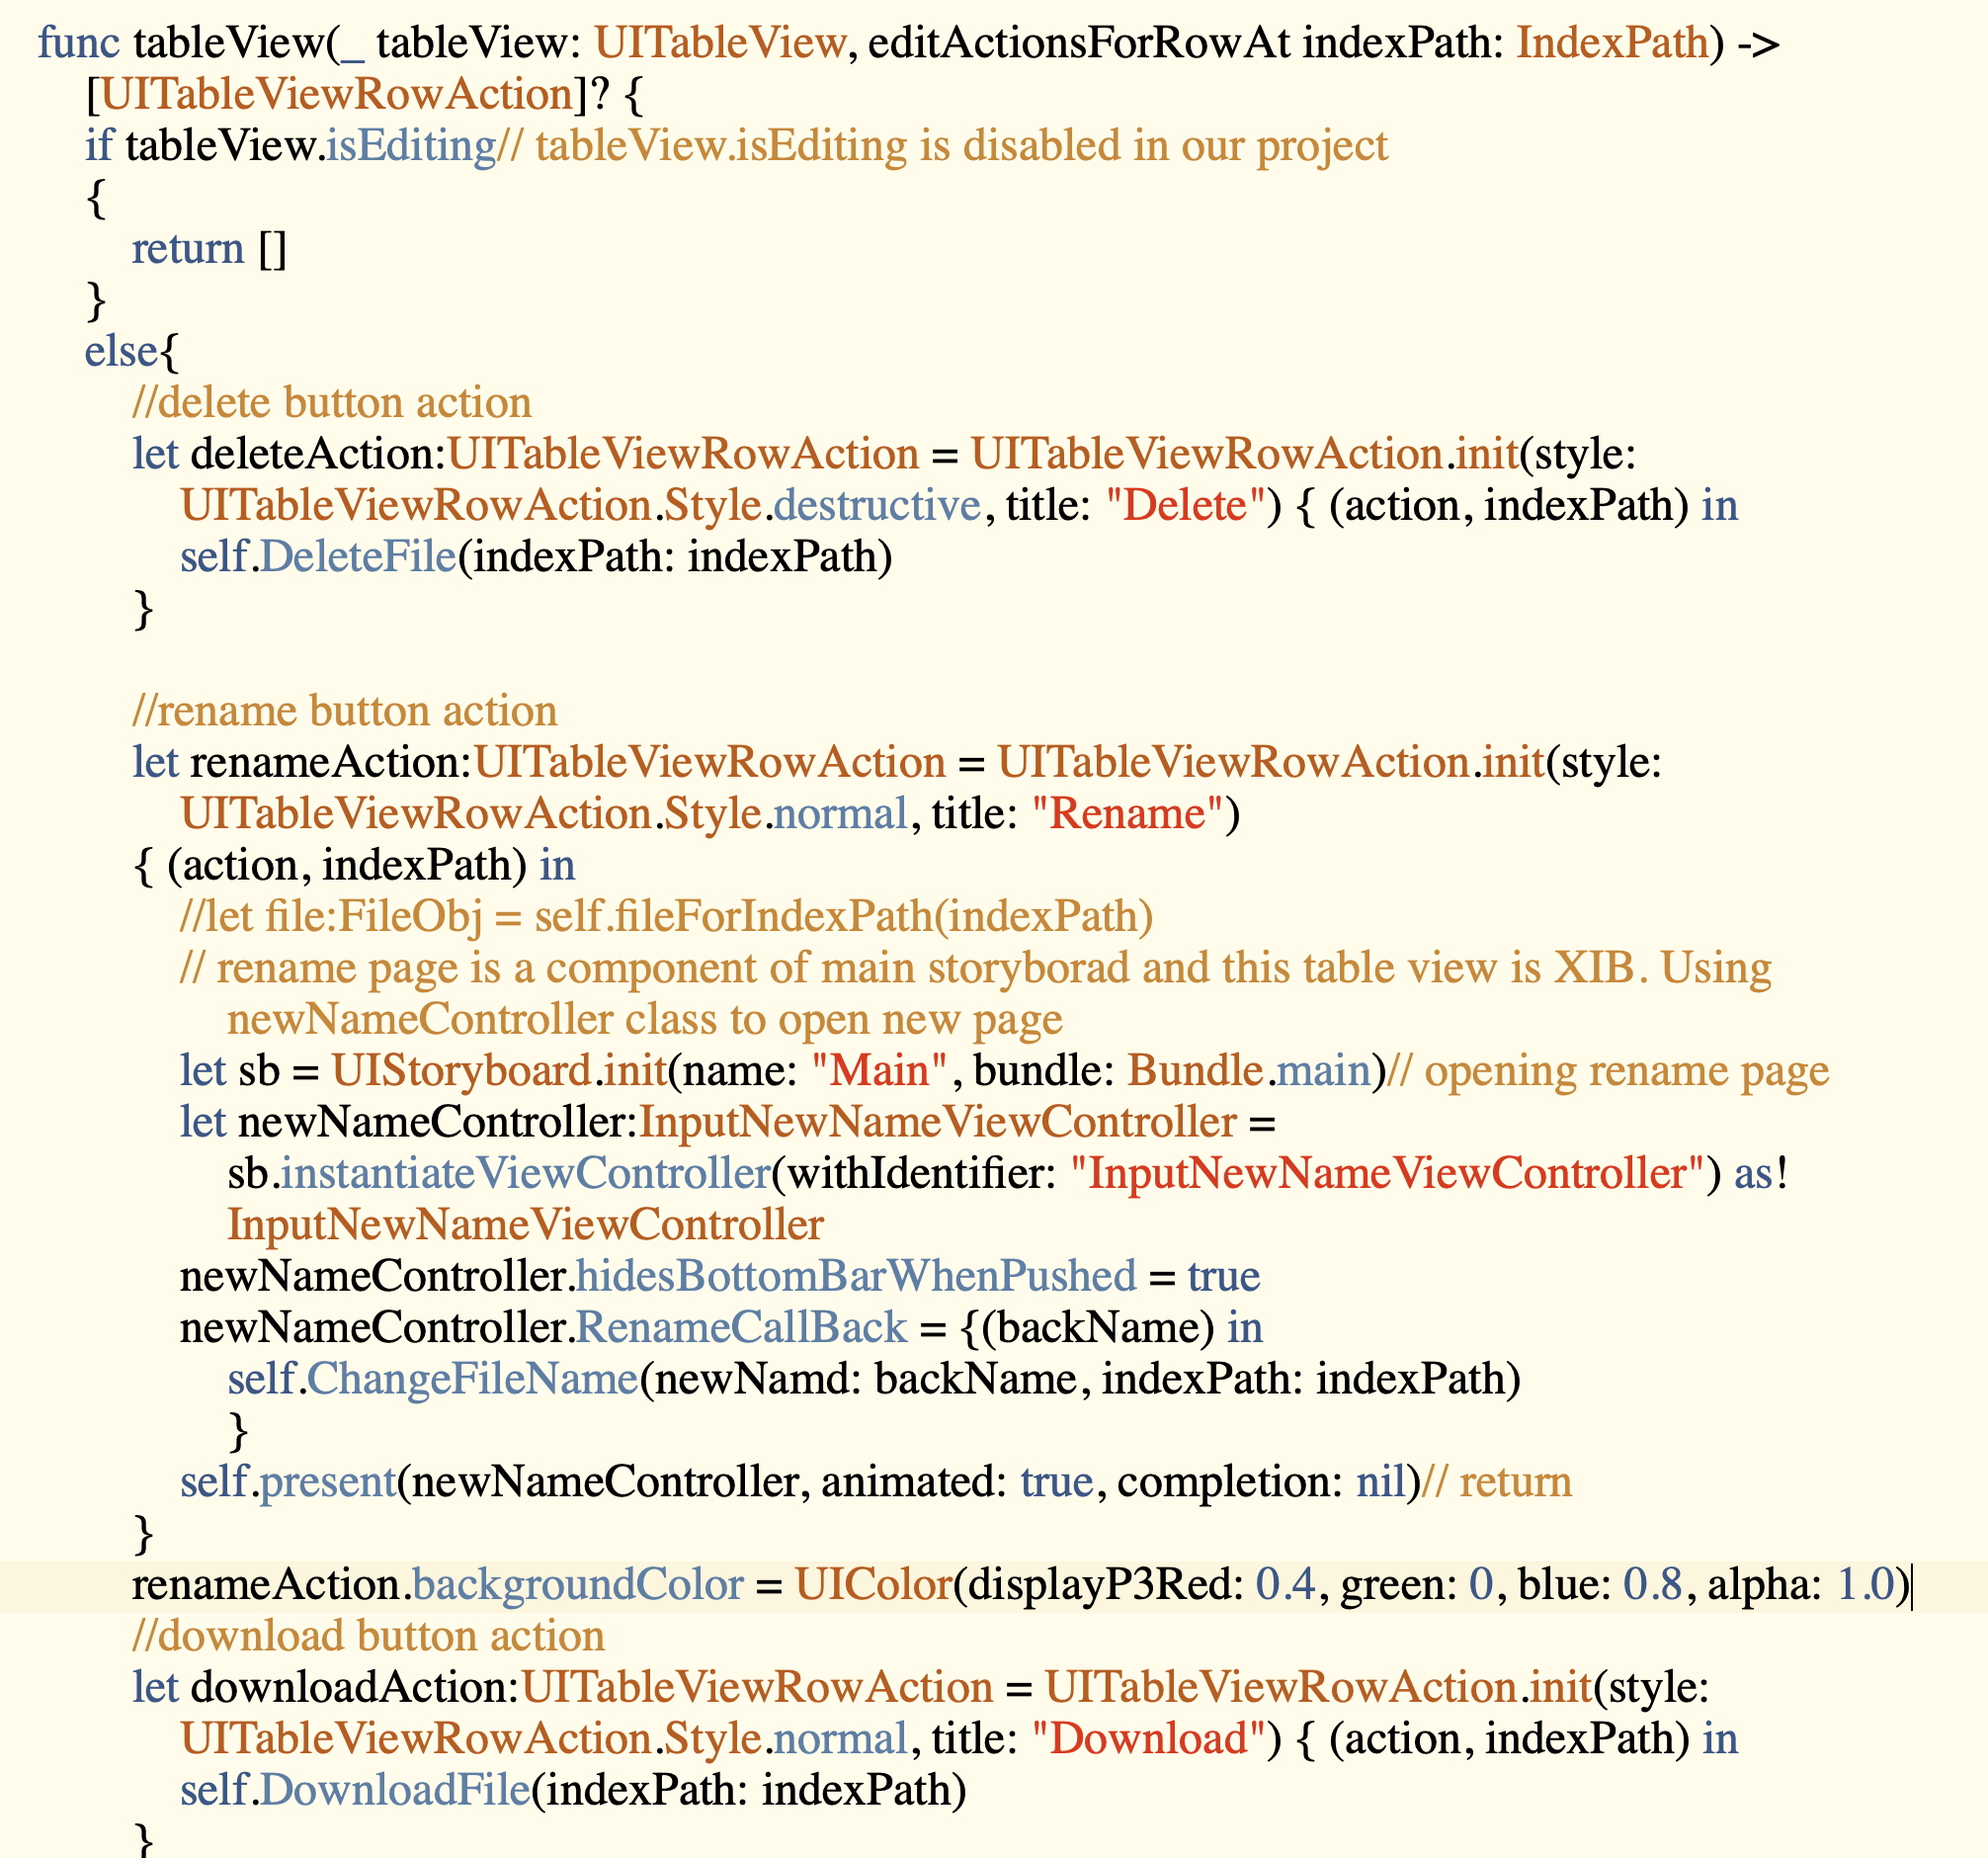
\includegraphics[width=9cm]{32.png}
\end{center}
\caption{Button actions in Cloud Page}\label{ex4}
\end{figure}

Another operation applied to Cloud page is multi-selecting and downloading files. Firstly by activating the multi-select function of TableView cells, then iterate each file in the file list (saving as a NSMutableArray) and call for HTTP to download one by one. Figure \ref{47} below demonstrates the code snippet of this part. 

\begin{figure}[H]
\begin{center}
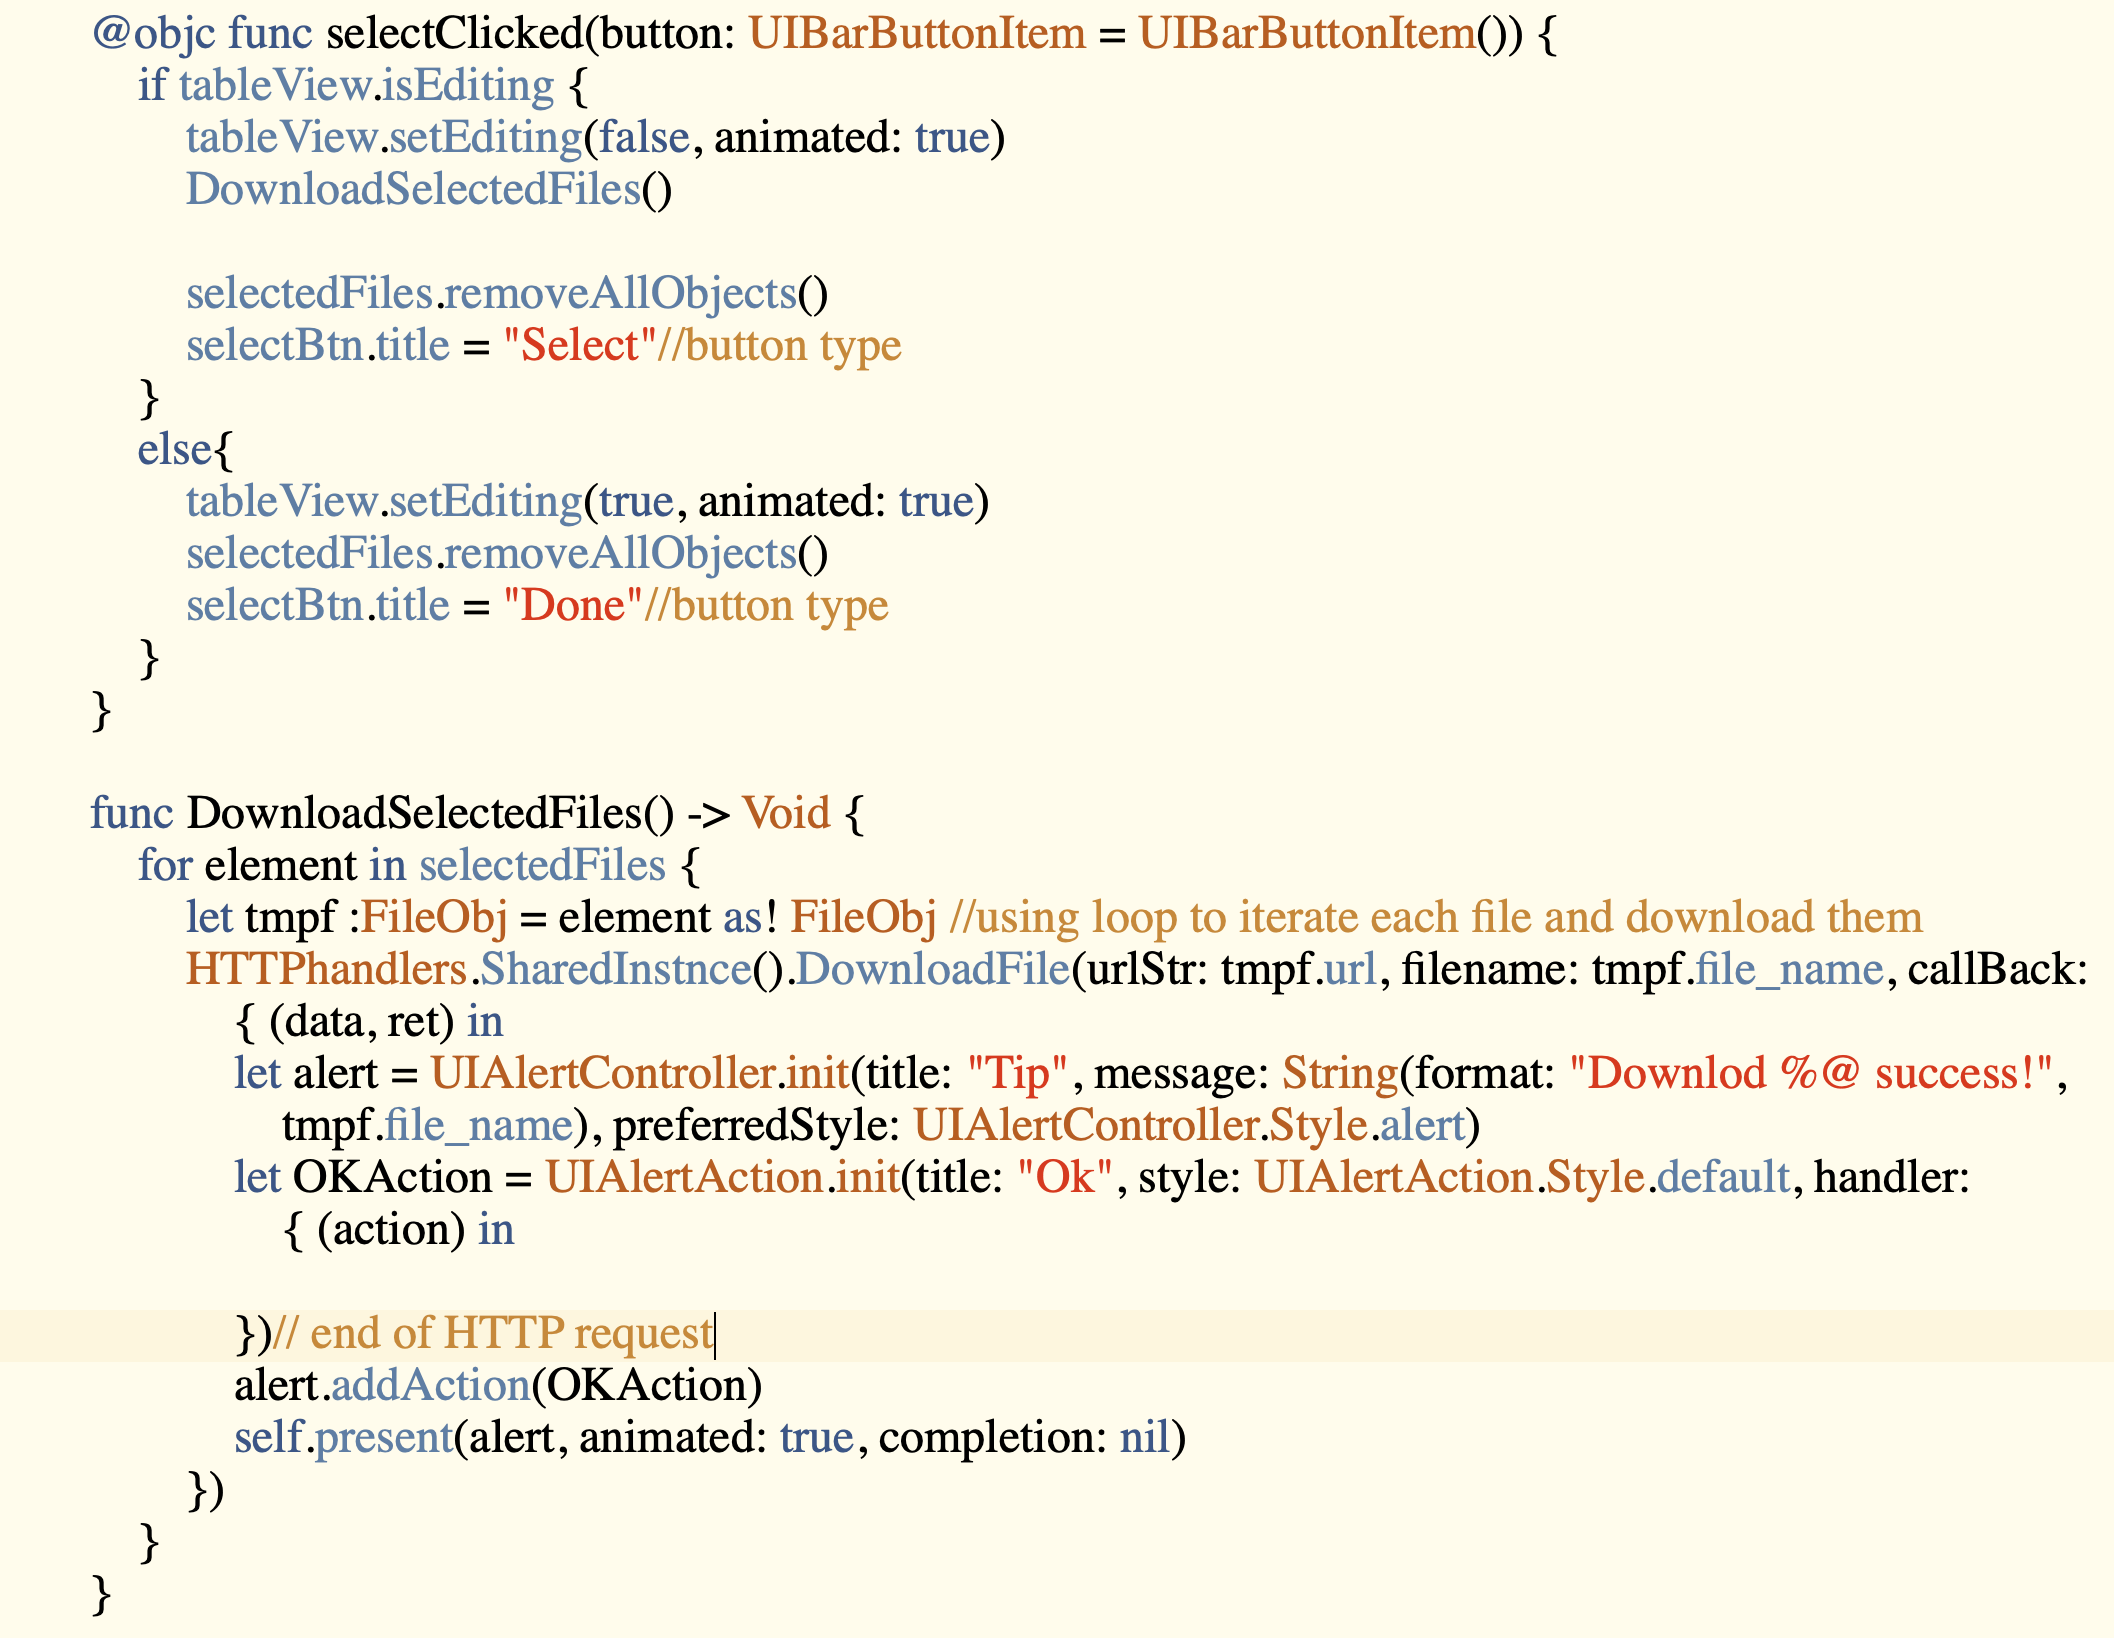
\includegraphics[width=9cm]{35.png}
\end{center}
\caption{Multi-select and download files}\label{47}
\end{figure}

\subsubsection{Selecting and Uploading Photos}

The navigation menu of the mobile client is actually another TableView that is cropped and has a sliding transmission to the Home View Controller. Since all the XIB files (custom TableView) we mentioned above are a kind of class. They can be called directly with the help of notification and observation functions in Swift, a Photo album is an exception. The view controller is extended in this part to open the local album for users. Figure \ref{ex41} shown below is a code snippet of the Home View Controller extension, and it helps users to pick a photo then uploading the file to the server. 

\begin{figure}[H]
\begin{center}
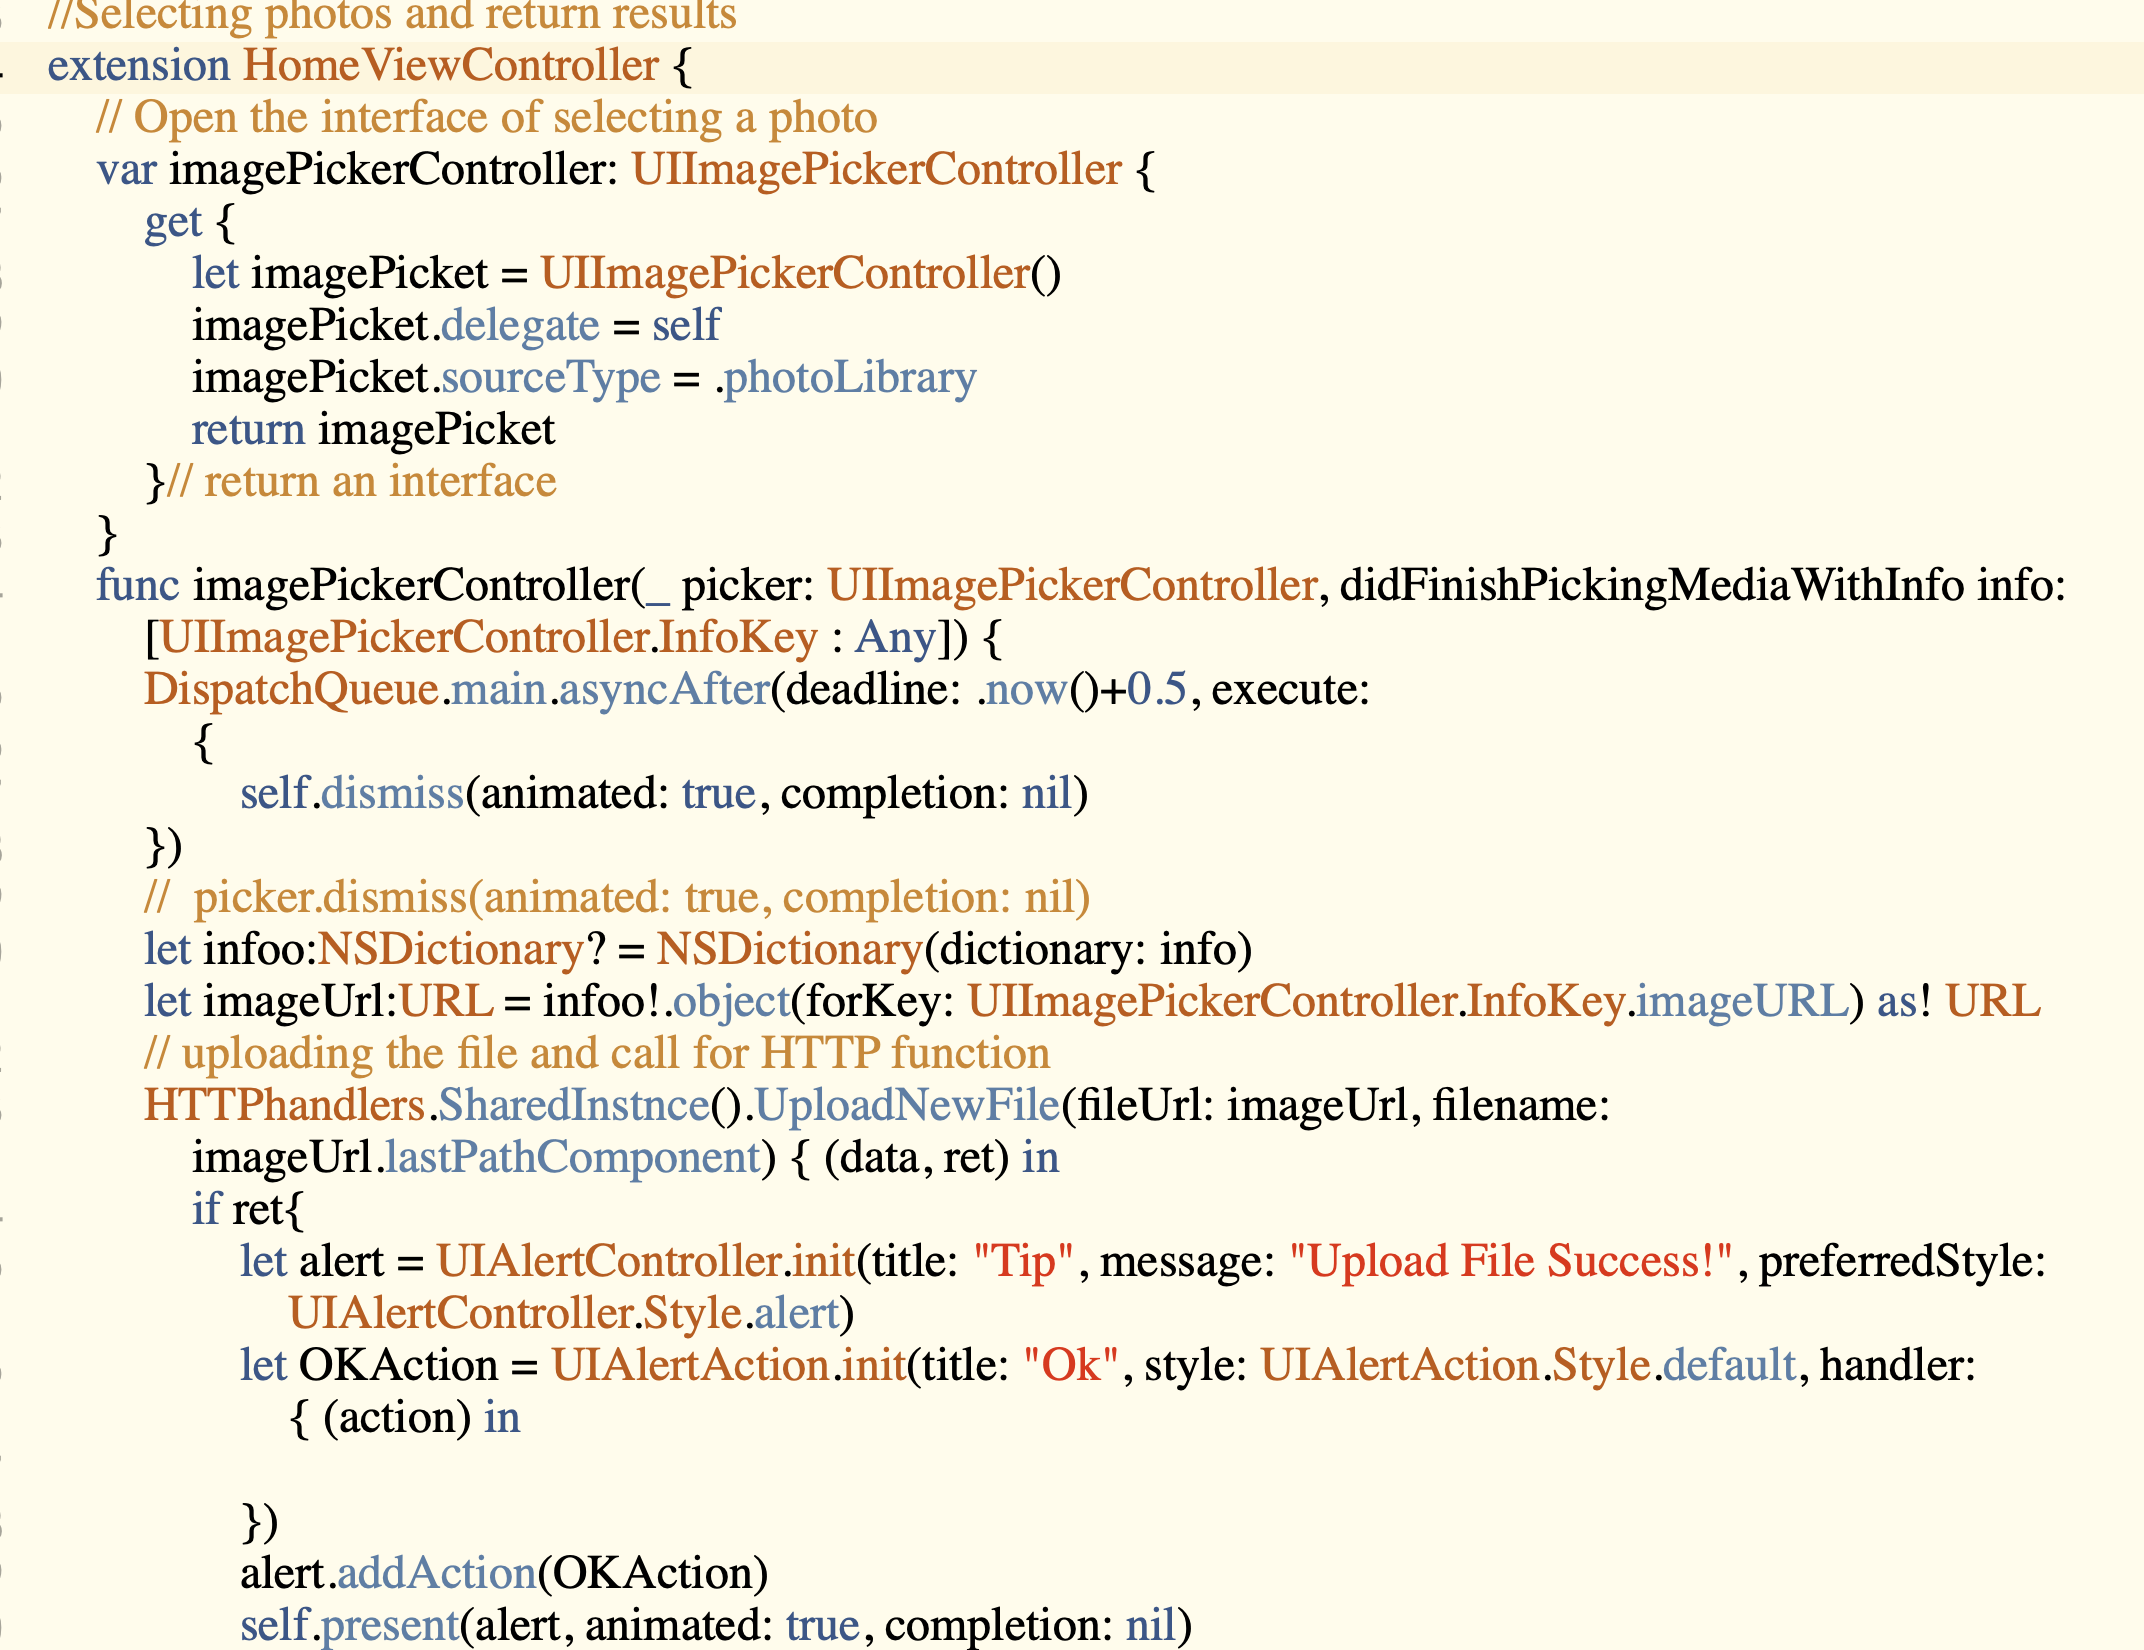
\includegraphics[width=9cm]{33.png}
\end{center}
\caption{Home View Controller Extension}\label{ex41}
\end{figure}
 
\subsubsection{Search Bar}

Search bar function is achieved by extending the TableView with UISearchBarDelegate and UISearchControllerDelegate. A function named 'search controller is active' helps us to ensure the status of a search bar, which is very important when performing fundamental operations. Since the parameters used for specifying a file is different in Table Cells and a Search result. Figure \ref{ex42} shows the differences between those two situations.

\begin{figure}[H]
\begin{center}
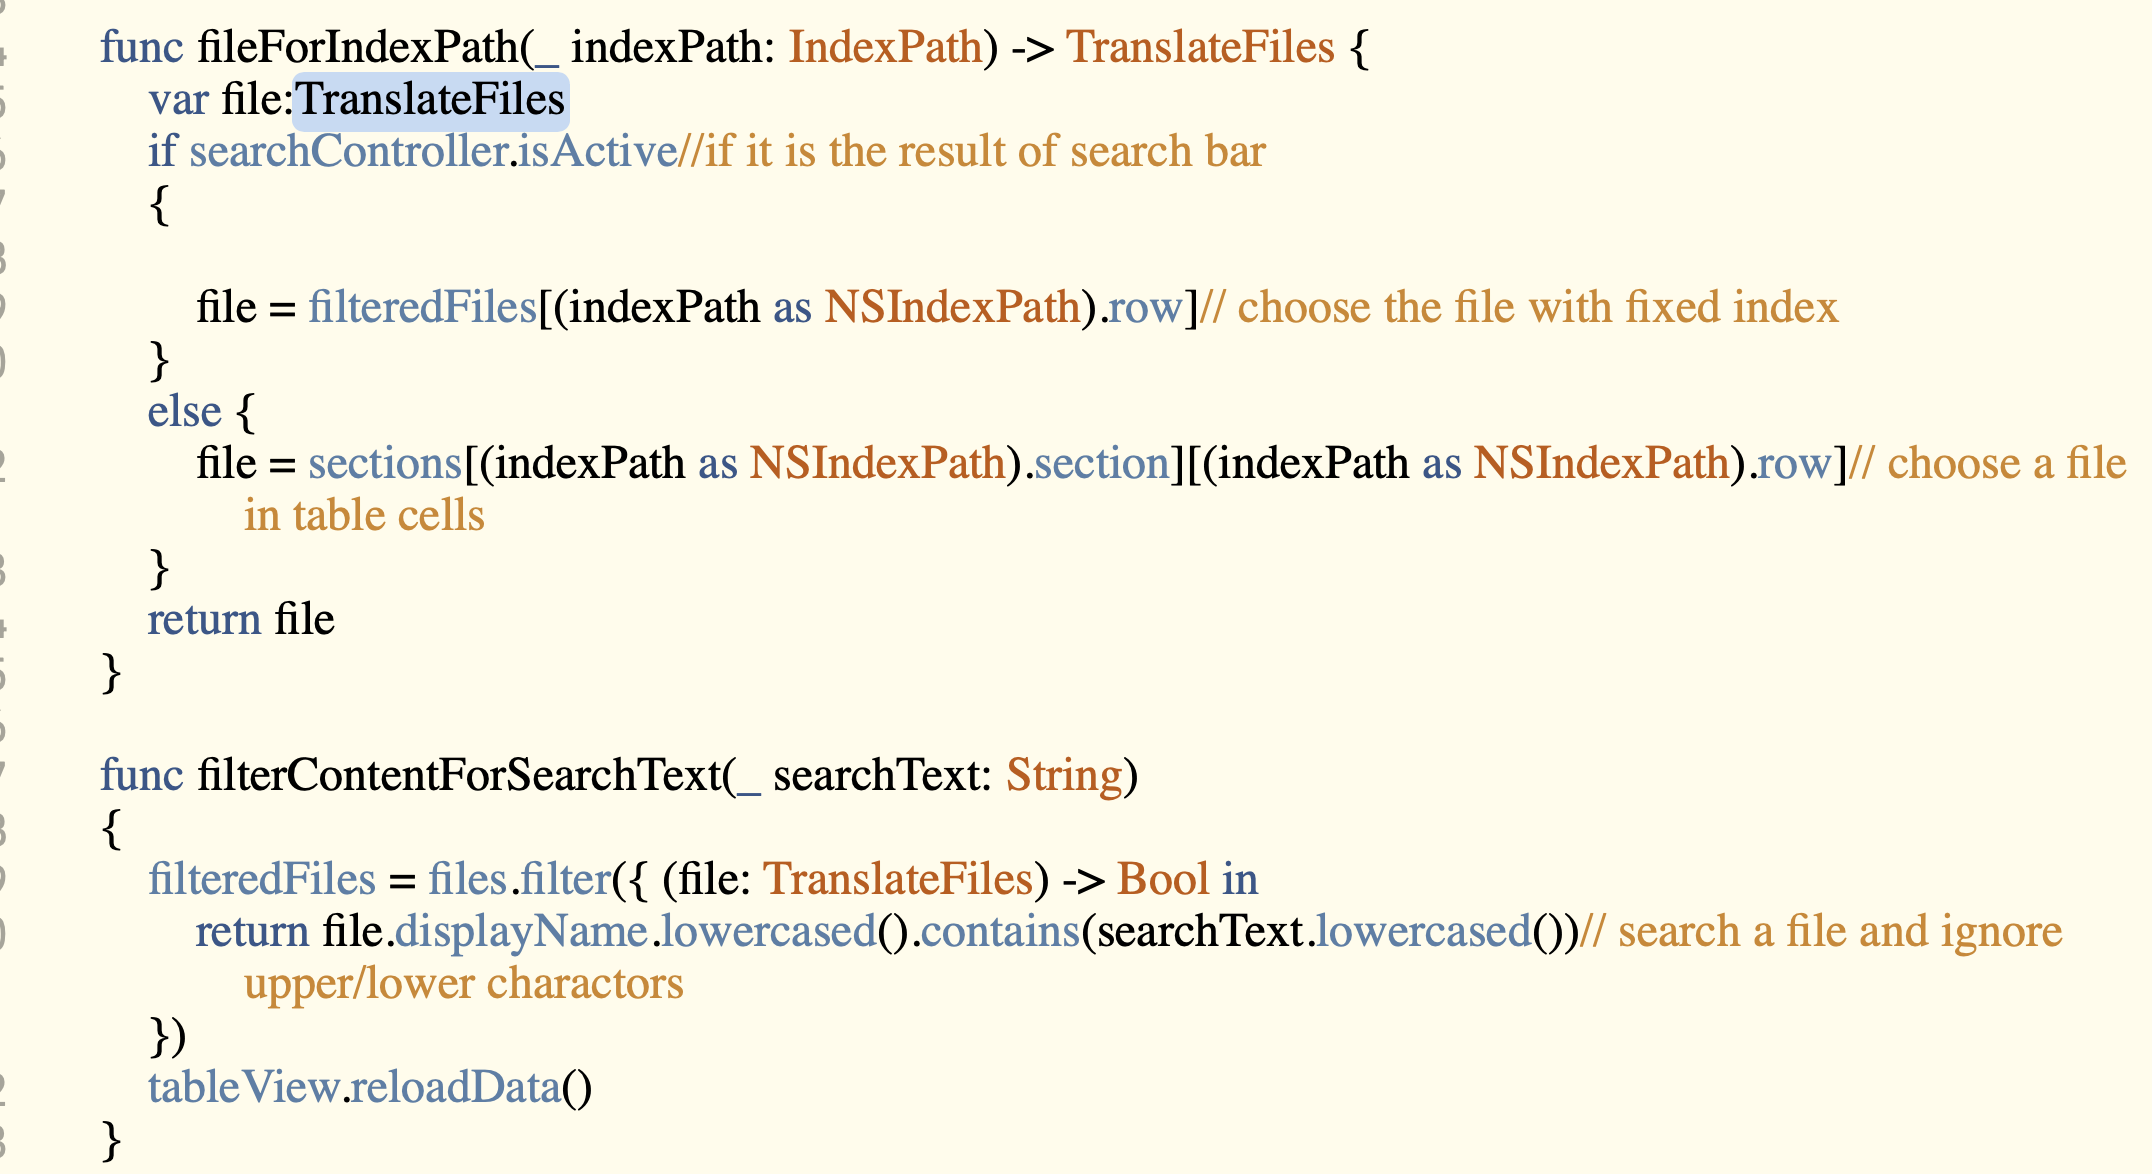
\includegraphics[width=9cm]{34.png}
\end{center}
\caption{Different parameters filters based on search bar}\label{ex42}
\end{figure}

\subsubsection{Handling Conflicts Locally}

\paragraph{Upload Conflicts}\mbox{} \\

\begin{figure}[H]
  \centering
  \subfloat[File upload Successfully]{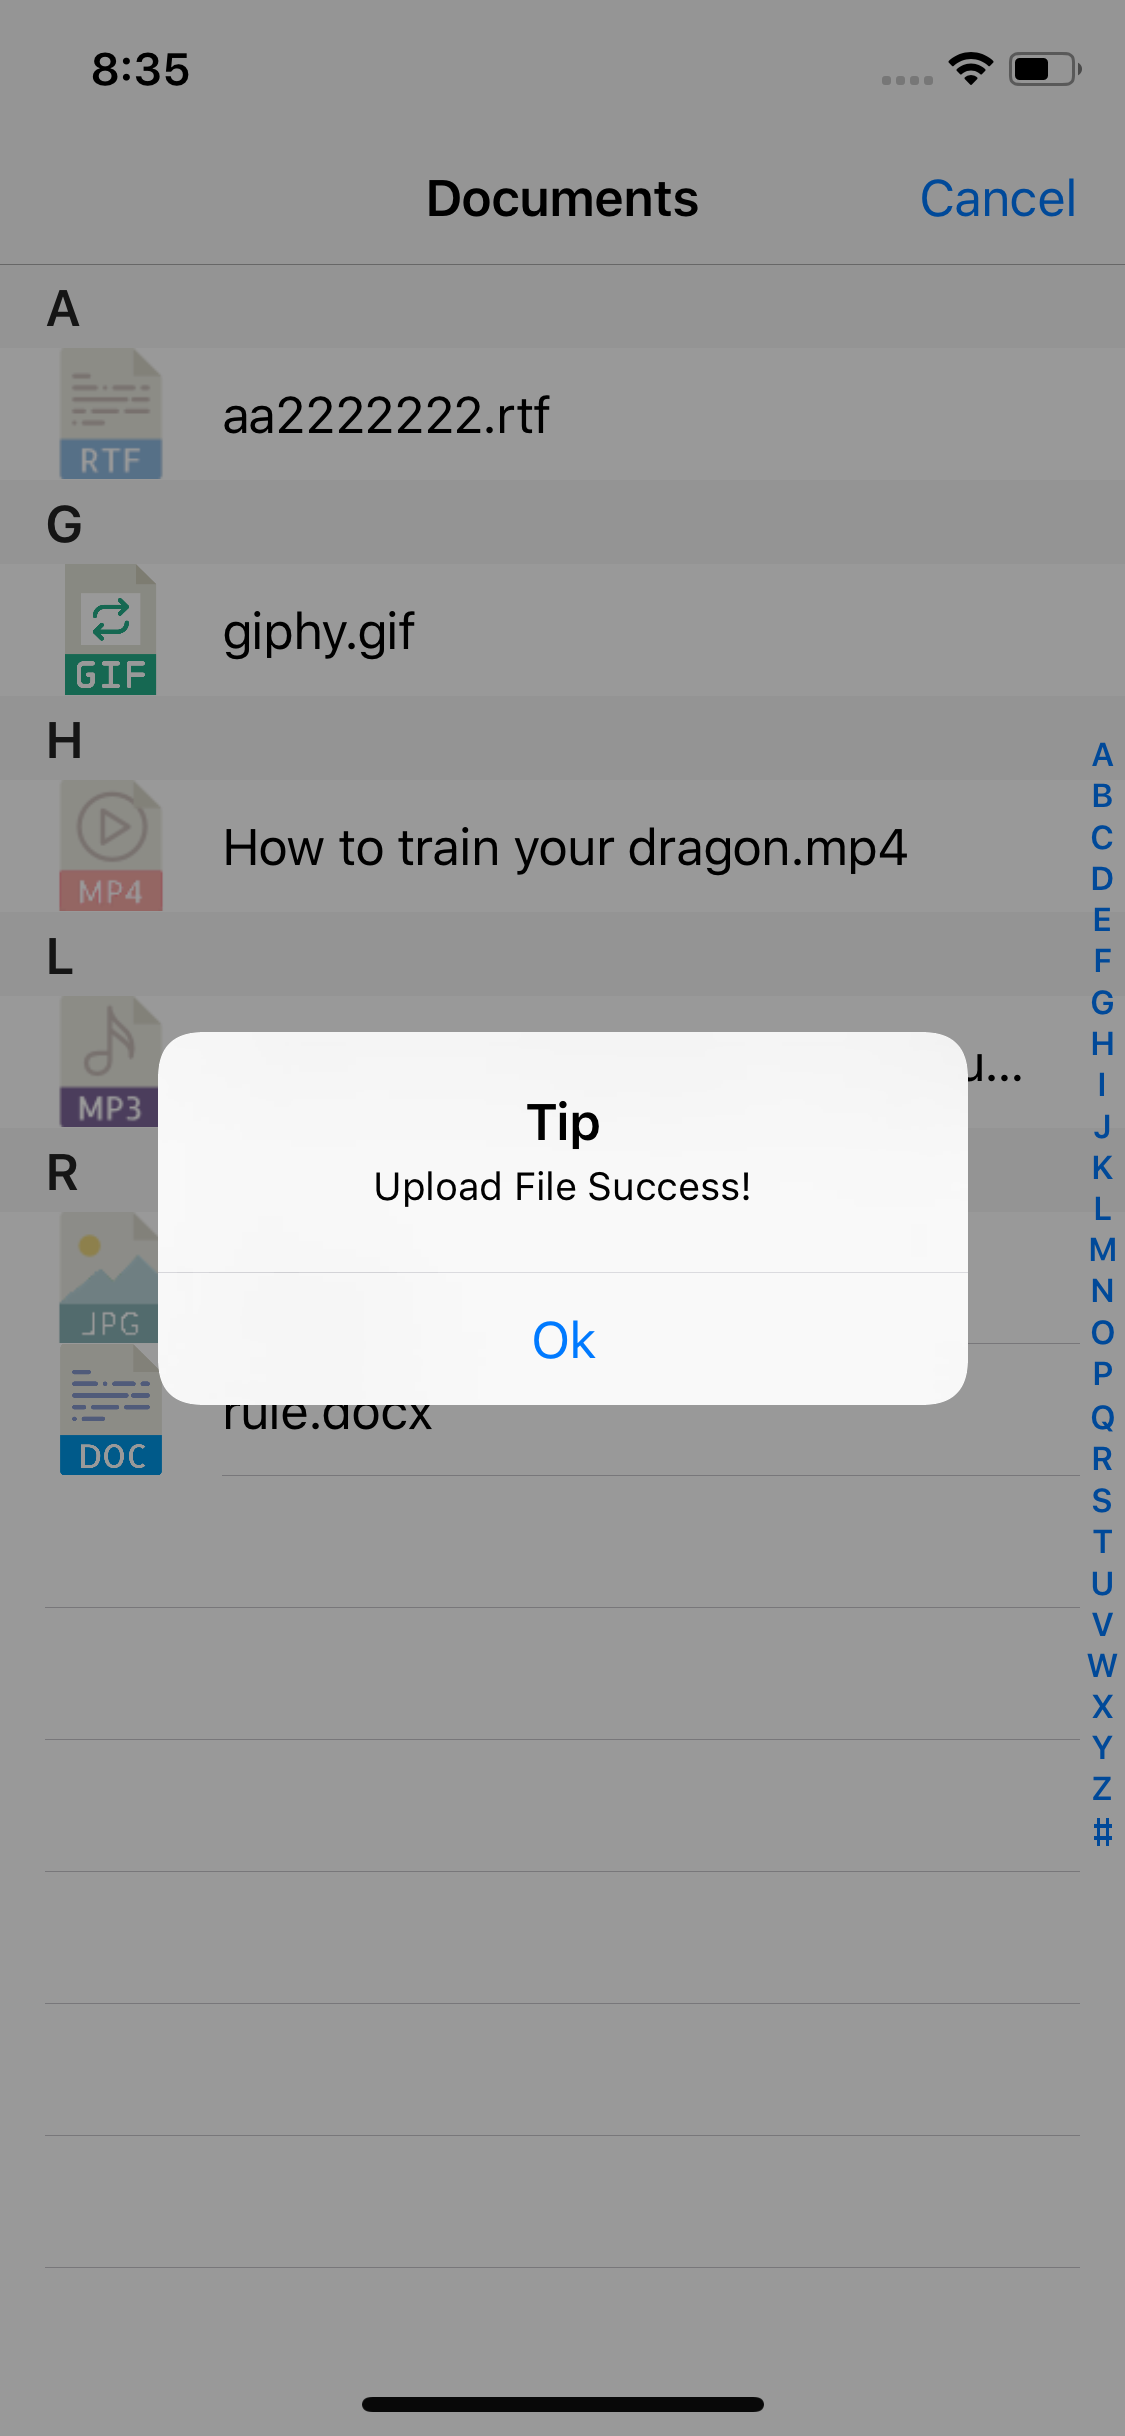
\includegraphics[width=0.19\textwidth]{37.png}\label{fig:f91}}
  \hfill
  \subfloat[Upload the same file will fail]{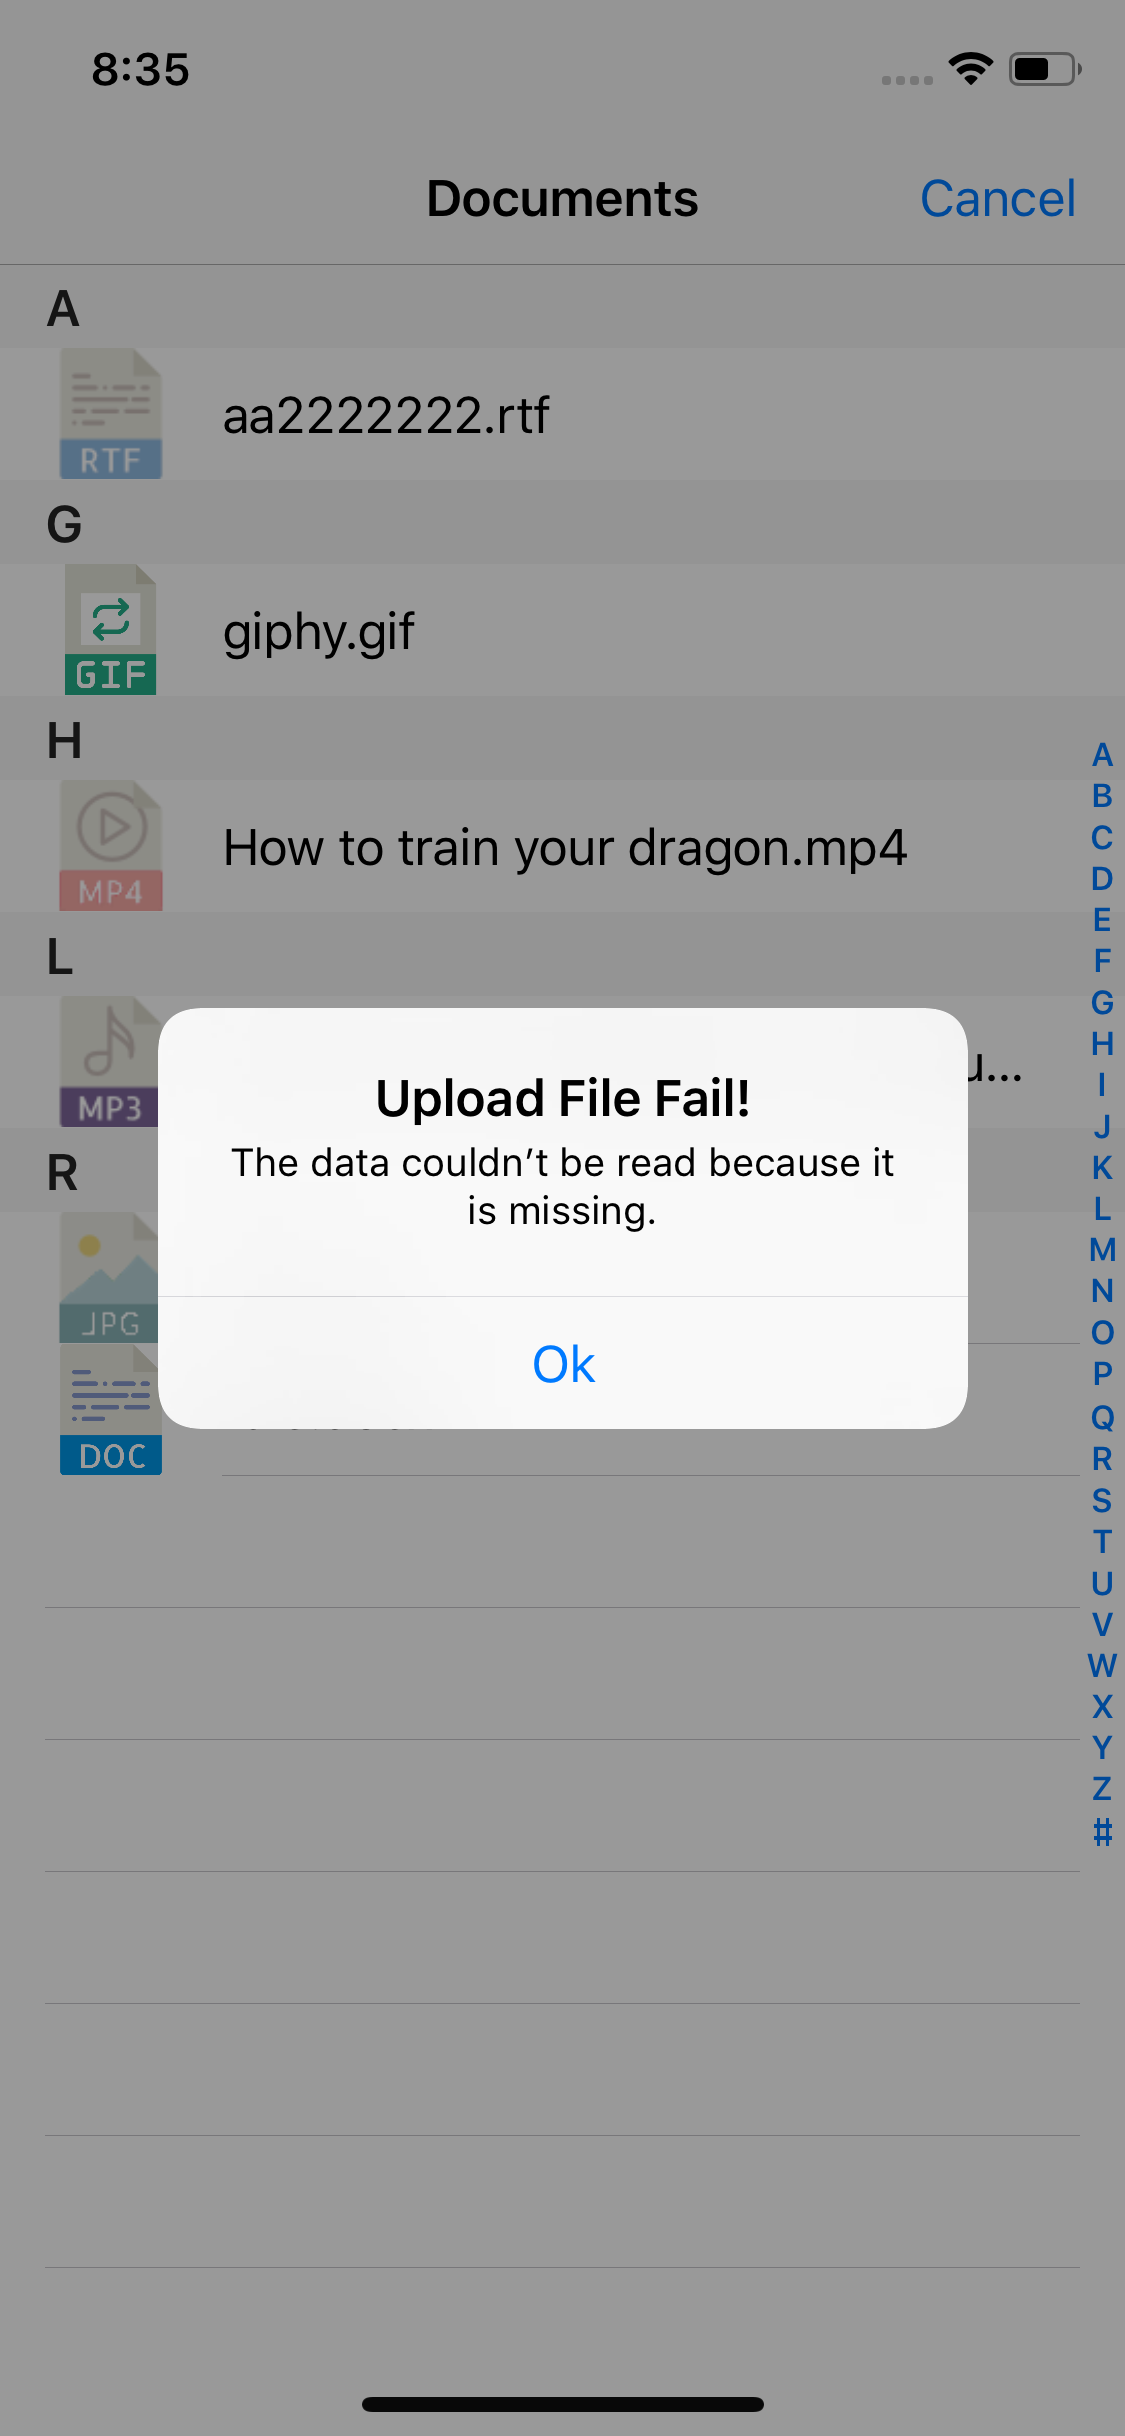
\includegraphics[width=0.19\textwidth]{38.png}\label{fig:f92}}
  \hfill
  \subfloat[Version Comparison]{
\includegraphics[width=0.19\textwidth]{40.png}\label{fig:f93}}
  \hfill
  \subfloat[Upload a big file will fail]{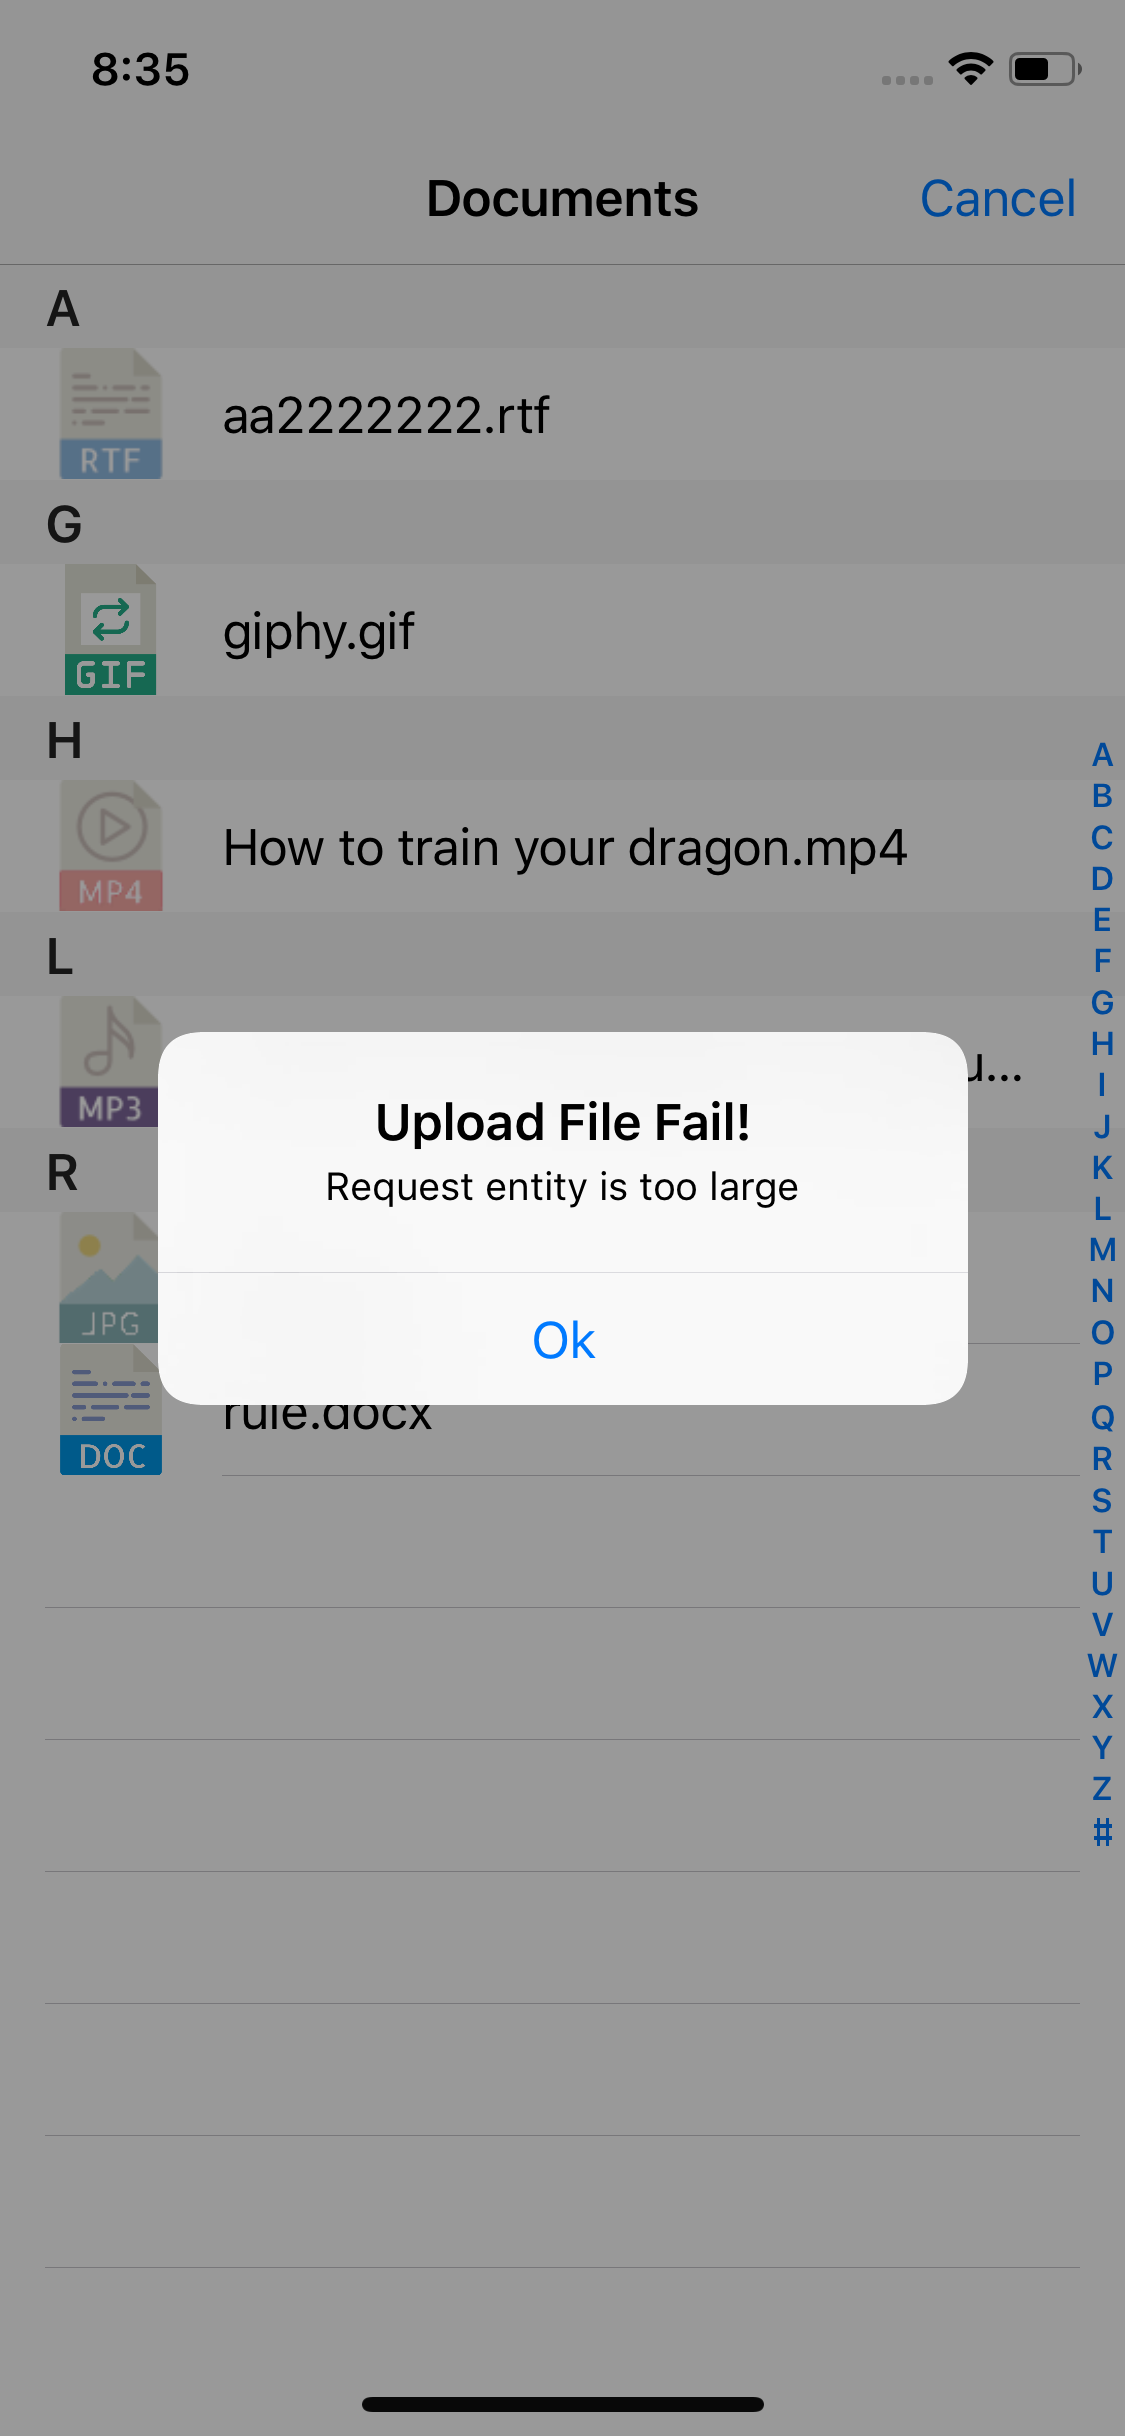
\includegraphics[width=0.19\textwidth]{39.png}\label{fig:f94}}
  \caption{Uploading Conflicts}
\end{figure}

One of this mobile client deficiencies is that the alert window just decodes the message sent by server. When dealing with conflicts, all the information is notified by server via HTTP response. Figure \ref{fig:f91} shows upload an image successfully. Figure \ref{fig:f92} shows when the user upload the same file as \ref{fig:f91}, server will give a failure response. Figure \ref{fig:f93} concerning the question of latest version file, this problem will also cause a failure in uploading. Finally, if a user upload a file exceeding the size limitation of server, failure response will be shown as an alert. 

\paragraph{Operational conflicts}\mbox{} \\

Mobile client can be installed in various iPhone models. Testing have been done in iPhone 5(s), iPhone SE, iPhone 6(s), iPhone 7, iPhone 8, iPhone X, iPhone XR, IPhone XS and all the plus versions in simulators supported by Xcode. However, It is found that conflicts would happen if one user was editing the name of a file and another user deleted it. Thus, the mobile client use a Boolean value to check the status and avoid operational conflicts. Besides, if a user download the same file for more than once, Tips as "download successfully" will be shown but in fact it won't change the Local Files.  


\subsection{Desktop Client}

\begin{figure}[H]
\begin{center}
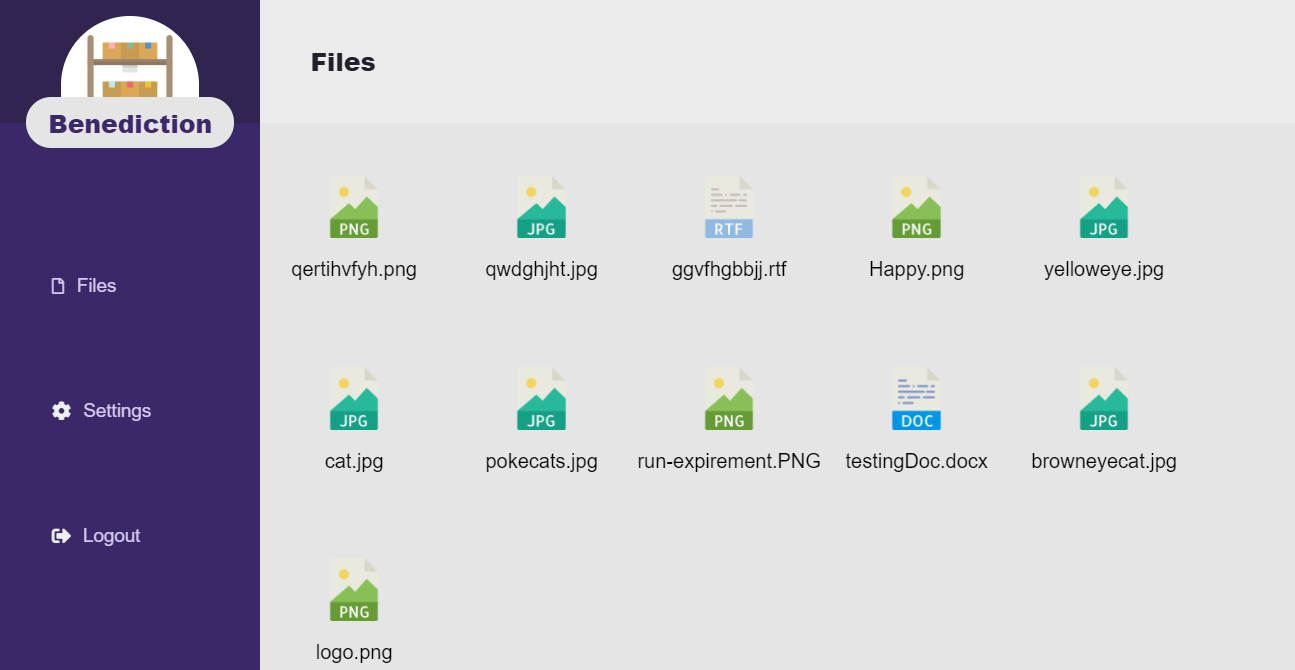
\includegraphics[width=12cm]{webui.PNG}
\end{center}
\caption{Web application User Interface}\label{ex4}
\end{figure}

\subsubsection {Front-End Application}
The application uses react and electron to run. It will need to start the react-script in order to render the UI and run this on electron to allow the Node.js function properly. Electron is a JavaScript-based framework which allows it to be available across all platforms, due to the web technologies that are supported by all platforms \cite{c4}. This framework helps to develop cross-platform application much more straightforward than having to deploy the app using different languages. It also allows Node.js to work with HTML,CSS and JavaScript to develop for both client-side and server-side application.

Websocket is used to keep the web application run in real-time. It provides a persistent connection between a client and server to allow data to be send over at anytime \cite{c13}. Below is the variable and function used to establish a websocket connection.

\begin{figure}[H]
\begin{center}
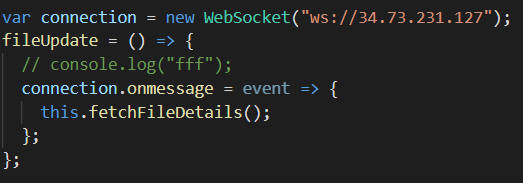
\includegraphics[width=6cm]{websocket.PNG}
\end{center}
\caption{Initialising WebSocket connection}\label{ex4}
\end{figure}

With websocket connected, the UI will retrieved data from the server automatically without the need to refresh the page. Whenever there are changes made, the websocket will ensure that there is a low latency connection that can support data transfer initiated by both client and server. This eliminates the problem of transferring large amount of data and increasing latency in order to keep the application running smoothly.

\subsubsection {Front-End Authentication}
This is a core function that ensures all users must be authenticated and logged in before accessing the web application.
In the code, there is a \emph{user} object that stores the user's username and password in order to check for their rights in entering the application. \emph{AuthService.jsx} file is used to fetch user's input and sends it to the back-end server via API. When a user have sign up to the system, the system will alert the user that they have successfully registered and will redirect the user to the login page automatically. Additionally, when the registered user is logged in, a token is assigned to them from the API server. This allows them to fetch the data using the token (within timed session) instead of using their username and password to authenticate each protected data.
When logged in, the token is saved in the local storage for further usage and fetching data from the server. The token will get cleared when the user is logged out of the application. This is shown by the figure below.

\begin{figure}[H]
\begin{center}
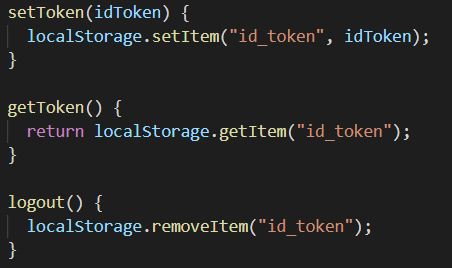
\includegraphics[width=6cm]{tokenAuth.PNG}
\end{center}
\caption{Setting,getting and removing token.}\label{ex4}
\end{figure}

A small browser library (jwt-decode npm package) \cite{c15} is used to help decoding the token in order to send the required authorisation headers to the API server. This is done by setting the authorisation header to \emph{Authorisation: Bearer xxxxxxx.xxxxxxxx.xxxxxx}. This is shown by the figure below.

\begin{figure}[H]
\begin{center}
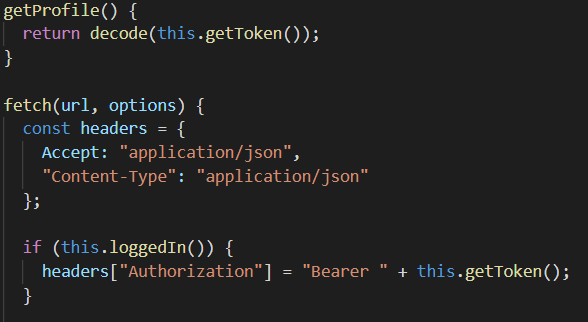
\includegraphics[width=6cm]{decodeToken.PNG}
\end{center}
\caption{Decoding token to set authorisation header}\label{ex4}
\end{figure}

\emph{WithAuth.jsx} file checks the state of the user to ensure that the user is logged in before accessing the main page. It relies on the data retrieved from \emph{AuthService.jsx} file to check the state of a user - whether the user is authorised or is currently logged out of the system.

\begin{figure}[H]
\begin{center}
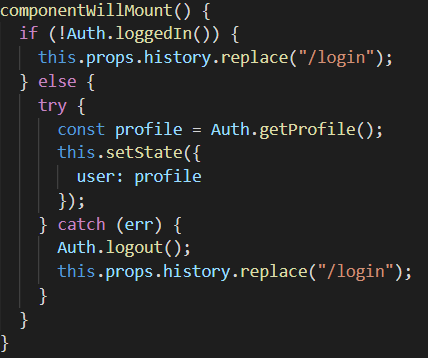
\includegraphics[width=6cm]{withauth.PNG}
\end{center}
\caption{Authorisation state of a user}\label{ex4}
\end{figure}

\subsubsection {Upload and Download Files}

\begin{figure}[H]
\begin{center}
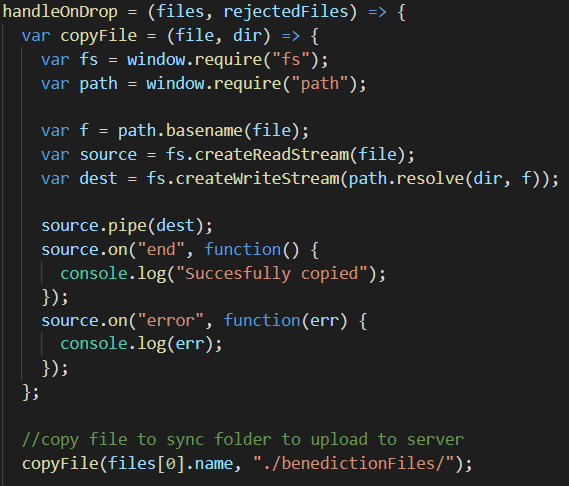
\includegraphics[width=6cm]{uploadDrop.PNG}
\end{center}
\caption{Upload file function}\label{ex4}
\end{figure}

To upload files onto the server, the user can either drag files into the UI or into the local file directory created by the web application. In the figure above, is a function with Node.js that handles the file that the user has dragged into the UI. \emph{copyFile} function make sure that the file is copied into the \emph{benedictionFile} folder to trigger the automatic upload function and sync it to the server.

For downloading a file, the user can double-clicked on the file element and this will download the file to the local sync folder (\emph{benedictionFiles}) using Node.js. This ensure that only files the user wanted will be download to their local machine and not every files on the server.

\subsubsection{Improvements}
From the UI design shown in section 3.2.2, there are still some implementation that were not included in the final UI. This includes displaying the user profile on the top right and syncing bar on the bottom right of the UI. This is due to the implementation were a little bit behind schedule. Nevertheless, these 2 components does not have any effect on the main goal which is allowing the user to upload/download file from the server and sync to their local file directory.

Moreover, set timeout could also be implement on the authorisation functions as it automatically log the user our if the user is inactive or have closed the application.

\subsection{Back-end Server Application}

\subsubsection{Real-time Communication: WebSocket}
\begin{figure}[H]
\begin{center}
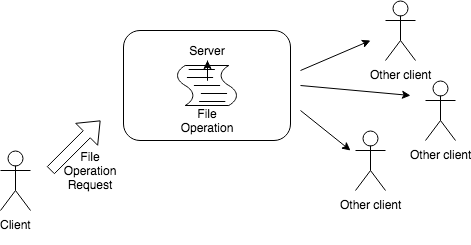
\includegraphics[width=9.5cm]{Backend_Diagram_WebSocket.png}
\end{center}
\caption{Diagram for WebSocket}\label{ex4}
\end{figure}
To achieve the requirement of synchronization of files. All the clients should be able to receive all the data in real-time. As a result, a real-time communication protocol should be applied in the project. In order to let the mobile client and the desktop client to be supported in the same solution. The team chooses WebSocket.

WebSocket is a protocol for full-duplex communication over a single TCP connection. WebSocket makes data exchange between client and server simpler and allows server to push data to client actively. \cite{c6}In WebSocket API, browsers and servers only need to shake hands once to create a persistent connection and carry out bidirectional data transmission.

The events broadcasted by WebSocket service should include all the event related to file changed on server. As the result, the team implemented:
\begin{itemize}
  \item File Update
  \item File Locked
  \item File UnLocked
  \item File Deleted
  \item File Created
\end{itemize}
All of the events broadcasted by the server is in the same structure that specify the name of the event and the data related to the event.

\subsubsection{Security: JSON Web Token}

To allow every client to process the authorization, a general standard should be selected. After conduct research among different approach, the team decides to use JSON Web Token as the solution for this project.

JSON Web Token (JWT) is a compact, URL-safe means of representing claims to be transferred between two parties. There are several advantages to use JWT as the solution.\cite{c7} First, High security to prevent token from being forged and tampered with Self-contained to reduce storage overhead. Second cross-language, multi-language implementation Support expires, publisher validation.
Of course there are still some disadvantages for using JWT,such as the message body can be decrypted to plain text by base64. Besides, JWT is not suitable for storing large amounts of information, and unexpired JWT can not be abolished.

The team use a Node.js module called node-jsonwebtoken to achieve the objective. To integrate the module into the Express framework, another module called express-jwt is used as a middleware that check the authorization before the request is processed by the function in the controllers. 

An JSON web token is generated when the user makes a log in request to the server. Once the server finishes the password and username checking with MongoDB, the server would generate a token based on secret string and the id of the user. After logging in, the client should put the token in the header in order to provide authorized evidence to the server application. 

\subsubsection{Security: MD5 Hashing}

In order to avoid password to be exposed once the database is hacked, the way of storing password should be guaranteed to protect the data to be revealed. Hashing could provide as a solution to this requirement. The team chooses MD5 as the algorithm for hashing. 

 MD5 is an implementation of information digest. The MD5 arbitrary length of plain text string generates 128 bits of hash value.Information digest generates a hash value of plain text content according to certain rules. Even if the plain text message changes only a little bit, the result will be totally different.

The underlying principle of MD5 algorithm:
Simply summarized, the process of MD5 algorithm is divided into four steps: 
\begin{itemize}
 
\item Processing the original text
\item Set the initial value
\item cycle processing
\item Stitching results

\end{itemize}

In the implementation, the team protects the password by, firstly, hashing the password in the endpoint of registration. Secondly, when the user tries to log in, the password would be hashed and then compared to the data in the database. Also, for every endpoint to offer the information of user, the endpoint would avoid offering any information related to the password.

\subsubsection{File Conflict Solution}

\begin{figure}[H]
\begin{center}
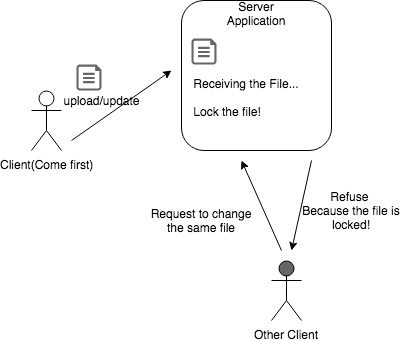
\includegraphics[width=9cm]{Backend_Diagram_FileLock.png}
\end{center}
\caption{File Conflict Solution}\label{ex412}
\end{figure}

When more than two clients are trying to request the server to do operations on files at the same time, a conflict file will appear on the cloud. To deal with this, the team applies file locking as a solution to the file conflict.

File lock is a mechanism to lock the document, which can control the reading and writing of files, prevent multiple methods of reading and writing the same file caused by inconsistency.

In the implementation, the server application uses a JSON file to store every details for files on the server. This includes the locking status of the file. So if an user is uploading a file, the file would be locked and any other user who intents to update the file would be refuse and receive a error message telling the fact that the file is locked.

Further, to avoid users to update a file and overwrite a new version of a file without noticing it, the API for updating the file is designed to require the user to offer the last version name of the file to ensure the user to know the latest version and confirm to overwrite the latest version of the file.

\subsubsection{Server Application Hosting: Google Cloud Platform}

To provide access for all the clients, the application should be deployed on a machine in the public network. The team selects virtual machine on Google Cloud Platform as the solution.

Due to the fact that Google is a powerful company with some advantages. The advantages include:
\begin{itemize}
    \item  Google has built a powerful platform, especially good at data applications. In order to support a popular network,GOOGLE is regarded as a leader in management
    \item  Sometimes it is considered a special supplier for specific tasks and used in conjunction with another major IaaS supplier.Instead of enterprise agreement discount, the longer users use it, the lower the price.
\end{itemize}
On the other hands ,the disadvantages exist.
\begin{itemize}
    \item Compared with the other two platforms, Google's cloud platform has more limited functions and other functions are still developing. 
    \item Compared with AWS or Azure, it is not mature, and users are in the basic stage.
\end{itemize}

To compare with other platform AWS is the largest and most mature public cloud IaaS provider, with the most advanced and diverse functions, and is a very safe choice.As the leader and creater of the market,the product of AWS always neoteric.Otherwise,there are some disadvantages below:
\begin{itemize}
    \item For customers,Amazon Market provides the most extensive third-party tools that can be used immediately on AWS and help consumers make good use of the platform.However,AWS product updates are too fast for users to keep up with the pace. Because of its wide range of functional functions, unskilled customers may be suppressed by the implementation principles. 
    \item Third-party professional service contracts are needed. The most important thing is that the unit price pricing is complicated through pre-purchase.
    
\end{itemize}

Compared with Microsoft, 
\begin{itemize}
    \item Microsoft Azure is an ever-expanding collection of cloud services that can help organizations cope with various business challenges. 
    \item Users can use their favorite tools and frameworks to build, manage and deploy applications on large-scale global networks at will.
\end{itemize}
There are some disadvantages exist either
\begin{itemize} 
    \item Although Microsoft meets most of Gartner's standards, it is neither mature nor friendly in some respects compared to the other two platform products and APIs.
    \item Unlike AWS, Azure does not have the concept of "region", which makes it difficult to backup data across regions. Despite its great efforts in open source and non-Microsoft technologies, Azure is still not the leader of open source, while AWS and Google's cloud technologies can bear the workload originating from open source.\cite{c8}
   
\end{itemize}

Overall, Google has built a powerful platform, especially good at data applications. GCP provides virtual machines, container engines and registries, as well as Cloud Functions. It has an object cloud storage service, cloud SQL plus Cloud Bigtable and cloud data storage, and the last two are NoSQL databases. Cloud Spanner is a relatively new highly scalable relational database service. Google is the best choice for this team to use.

By using virtual machine on google, the team can easily scale the service if needed. In addition to that, the platform offer services include bind an ip address with the machine that help the service to be able to provide service in a fixed location on the Internet.

\subsection {Testing}

The development application was tested in a number of ways starting with \emph{white box testing} where each developer tested independently before pushing commits to Git for review. Independent testing enabled each group member identify any defects and or bugs before committing code that would be merged with already working code. Identified defects or bugs would have to be corrected and code re-tested before pushing it to Git.
After pushing each commit to git – \emph{black box testing} according to story journeys as seen below and functional specifications would be carried. Additionally, reviewer(s) (another team member different to the code committer) would pull the committed code and test functionality to determine the code performs as it’s supposed to. However, before black box testing – peer review is done on the code to check for any coding standards and identifying or finding any bugs where possible. If the above identified any incorrect functionality, inconsistent coding standards or any bugs, the reviewer would notify the group member that pushed the code to pull and fix the issues, test and if corrected, push again. For mobile application development, the application was installed on the group members' iOS phones and functionality as well as appearance and crashing tested as a whole.

Once the above run smoothly, integration would be carried to connect back-end to front-end user interface. Once successfully connected, \emph{Integration testing} would be carried out at this point to evaluate the end to end communication between front-end and back-end modules. This would identify any faults between the two modules as well as evaluate the various interaction between different functionalities and how the work successfully together within whole system. 

Each group member is involved at every stage during testing from independently testing their own code to testing code pushed by others as well as integration testing of the whole system. Furthermore, a small number of students were used to test the system as a whole to identify any possible variations in the requirements specified. The feedback generated from these students was used to iterate changes to the system.

Black box, grey box combination and white box testing enable teams to benefit from the strengths of each approach and offset the weaknesses.

\subsubsection{Testing Cases}

\begin{itemize}

\item\textbf{File upload}
    \begin{itemize}
        \item{Test Scenario: Verify the function of uploading the file}
        \item{Test Case: Prepare a file to upload. In this test, a text file is created for the text.}
        \item{Test Step(s): make a POST HTTP request on the endpoint upload a file to upload the file.}
        \item{Test Result/Expectation: The file should be successfully uploaded in the file storage folder given a file id and version in the file.json in the file folder. The WebSocket event for a new file uploaded should be triggered}
        \item{Test Status: Pass}
    \end{itemize}
\item\textbf{File update}
    \begin{itemize}
        \item{Test Scenario: Verify the function of updating the file to update a file}
        \item{Test Case: Prepare a file to upload. In this test, a text file is created for the text.}
        \item{Test Step(s):}
            \begin{enumerate}
                \item{make a POST HTTP request on the endpoint upload a file to upload the file.}
                \item{change the content in the file}
                \item{make another POST HTTP request on the endpoint upload a file to update the file.}
            \end{enumerate}
        \item{Test Result/Expectation: The file should be successfully uploaded in the file storage folder given a file id and version in the file.json in the file folder. The WebSocket event for a new file uploaded should be triggered. After the second upload, the file in the folder should be changed and the version of the file should be edited. All the clients should receive notification by WebSocket for file update}
        \item{Test Status: Pass}
    \end{itemize}
\item\textbf{File rename}
\begin{itemize}
        \item{Test Scenario: Verify the function of renaming the file}
        \item{Test Case: Select a file on the server and change the name of a file on the server. In this case, the team uses the file they uploaded from the first test}
        \item{Test Step(s): make a POST HTTP request on the endpoint to rename a file on the server.}
        \item{Test Result/Expectation: The file specified should be successfully renamed}
        \item{Test Status: Pass}
\end{itemize}
\item\textbf{File delete}
\begin{itemize}
        \item{Test Scenario: Verify the function of deleting the file}
        \item{Test Case: Select a file on the server and delete the name of a file on the server. In this case, the team uses the file they uploaded from the second test}
        \item{Test Step(s): make a POST HTTP request on the endpoint to delete a file on the server.}
        \item{Test Result/Expectation: The file specified should be successfully deleted}
        \item{Test Status: Pass}
\end{itemize}
\item\textbf{User register}
\begin{itemize}
        \item{Test Scenario: Verify the function of registation of a new user}
        \item{Test Case: A set of user information is prepared. This includes the username to be testuser, password to be pwdtest, firstname to be Danny, and last name to be Yao}
        \item{Test Step(s): make a POST HTTP request on the endpoint to register a new user.}
        \item{Test Result/Expectation: The response should be successful with the user data just created, and a user should be created in the database.}
        \item{Test Status: Pass}
\end{itemize}
\item\textbf{User log In}
\begin{itemize}
        \item{Test Scenario: Verify the function of logging in of a user}
        \item{Test Case: The username and password from last test are used here to test the log in process.}
        \item{Test Step(s): make a POST HTTP request on the endpoint to log in a user.}
        \item{Test Result/Expectation: The response should include a token for the user's authorization in other HTTP request.}
        \item{Test Status: Pass}
\end{itemize}
\item\textbf{User Authorization}
\begin{itemize}
        \item{Test Scenario: Verify the authorization middleware to block the request without authorization}
        \item{Test Case: Nothing to provided as testing data set.}
        \item{Test Step(s): make a GET HTTP request on the endpoint to get all the information for all the files on server.}
        \item{Test Result/Expectation: The response should be an error response.}
        \item{Test Status: Pass}
\end{itemize}
\item\textbf{File Download}
\begin{itemize}
        \item{Test Scenario: Verify the download process of the file on the server}
        \item{Test Case: A file id is provided to specify the file to be downloaded}
        \item{Test Step(s):}
        \begin{enumerate}
                \item{make a GET HTTP request on the endpoint to get a file on the server.}
                \item{check the files stored in the local folder}
            \end{enumerate}
        \item{Test Result/Expectation: The response should be an successful response following a download to be started.}
        \item{Test Status: Pass}
\end{itemize}
\item\textbf{Upload Conflicts Handling}
\begin{itemize}
        \item{Test Scenario: Clients upload files in simultaneously }
        \item{Test Case: each client will get command window to re-upload or blocked to upload}
        \item{Test Step(s):}
        \begin{enumerate}
                \item{each client will download the same file into a local folder}
                \item{edit the file contents and re-upload with the same files name}
            \end{enumerate}
        \item{Test Result/Expectation: the command window pop-up successfully, induce clients to change the file name}
        \item{Test Status: Pass}
\end{itemize}
\item\textbf{Rename Conflicts Handling}
\begin{itemize}
        \item{Test Scenario: During renaming a file, the other clients delete the file}
        \item{Test Case: renaming finished a warning window pop-up and the renaming request will not send to the server}
        \item{Test Step(s):}
        \begin{enumerate}
                \item{client A rename the file id}
                \item{client B delete the file}
                \item{client A finish renaming work}
            \end{enumerate}
        \item{Test Result/Expectation: cannot find the file id in the server, the renaming request is rejected}
        \item{Test Status: Pass}
\end{itemize}

\end{itemize}
\subsection{Data Storage}
\subsubsection{MongoDB}

The team chooses MongoDB as its database solution. MongoDB aims to provide a rich document orientated structure with dynamic queries that you'll recognize from RDMBS offerings such as MySQL. MongoDB, a cross-platform NoSQL database, is the fastest-growing new database in the world. MongoDB documents are difinetly similar to the JSON objects. Field values can contain other documents, arrays and others.
\cite{c9}\newline 
By default, MongoDB pays more attention to high insertion speed and handles large-scale single tables than transaction security. Database expansion is very challenging, and MySQL table performance will undoubtedly decrease when the single table size reaches 5-10GB. MongoDB will be able to do this easily when you need to fragment and split your database. Reliable environment guarantees high availability. And then it use location-based data queries to search faster.Without a professional DBA and without structuring your data and joining queries, MongoDB would be our first choice. MongoDB is very suitable for class persistence. Classes can be serialized into JSON and stored in MongoDB.


\subsubsection{Table Scheme}

For the project, the team designed two tables to store the structured data. First, a table called user is to store all the data related to users' information. The fields include id of the user as the primary key, username, hashed password, first and last name of the user. Besides, A table called files is to store detailed information of files. This include the id of the file as primary key, version, locking status, file name, and the location of the file.

\subsubsection{Difficulties: Stability of Database Connection }

Due to the fact that the upload process of the files could be very fast, the data storage application should be able to update the locking status of file very fast. Further, If the the locking status fail to be changed, the result could be that a file to be locked forever, or a file to be overwritten by another conflict file. To avoid these situations, the data storage should be able to avoid failure on data updates. 

Regarding the problems addressed above, the connection between MongoDB server and back-end side application should be stable to reach the requirements. But there is no guarantee that the connection will always be stable. To solve the problem, the team decides to store the information of the files in a local JSON file. By using JSON files in the local machine, the applications does not require a stable connection between database server and back-end application server, and all the data can be managed easily.

\section{Teamwork}
Because of lack of communication in the original back-end sub team, the back-end team has spent almost a month researching different solutions and languages to choose for the back-end application without discussion between the members, this causes conflicts and no agreed solutions were decided. After receiving the feedback on the project initial report and presentation. The sub team for back-end development struggled to find conclusions on which languages to use and solution for real-time synchronization. Thus, after discussion as a team, an agreement was reached and roles were switched to further more development. This action effected the whole team in terms of time that would have been used for implementation of the project work. Two members switched roles as one had more experience on WebSocket as a real-time and Nodejs communication that was going to be used including JavaScript (Yao Te-Chien) while the other team member with less experience contributed to front end Nodejs (Isaac Muhumuza) implementing all the features related to file system on desktop client.

However, for the back-end team, due to the lack of experience of another member (Zhang, Yiwei Harper), even though Harper tried to contribute a few times, but the qualities of the code did not meet the standard therefore not integrating it with the code written by others, resulted in having zero contribution to the program. The code written by Harper each time could not successfully run and as a consequence, Yao Te-Chien finished all the back-end tasks on implementation alone. Harper mostly helped on describing the back-end knowledge in the report. 

For the mobile team; Yan Li and Jihye Hwang, the UI design has been decided, the team separate the job into tasks assigned to each member. Each member took one by one function and start working on their code. Once a task is done, the member will move to working on the next tasks. Li has some experience about iOS but this development is new for Jihye. Fortunately, Jihye used to C and C++ so she can handle the Swift language. The team has met three or four times a week. During the meeting, the members discuss, coordinate some part of the code, combined the code and solve the problem together.

As mentioned above, the members have switched between the back-end and desktop team. So the desktop team; Chayanit Krairit is responsible for developing the user interface part in React and Issac Muhumuza is responsible for developing the file system to sync with the server in Nodejs. With that said, Isaac was not familiar with Nodejs as he was fairly new to coding in web development, this cause the implementation phase to be slower than first planned in the Gantt chart. Nevertheless, he insisted on helping the team and learnt Nodejs from scratch in order to help weigh out the workload on the other team members.


\section{Evaluation}
\subsection{Possible Improvements on Team Work}
In terms of the team-working in this project, there are multiple improvements that can be made. Firstly, the division of the jobs can be more specific and the responsibilities of every member should be more clear. At the beginning of the project, the team is divided into three sub teams as back-end, mobile client and desktop client division. However, further division on tasks should be conducted earlier, so the members are assigned own duties from the start. This could offer more time for all the members to investigate any technology choices and learn skills required to complete project. Moreover, the dispute on the technologies to use should also be settled earlier so that more time can be spent on the developing the system. 

Secondly, the communication between the members, even though, the team has set up a team meetings every week to give an update of what each member has been doing but because the tasks were not clearly defined after switching to sub teams, which causes some members to have different approaches on developing their code. In addition, the team also have a group chatroom for members to ask or give their opinion on the project, however, some members were not actively responsive to messages which causes a difficulty in communication between the team. This is believed to cause the sub team switching and the delaying on development of this project. 

Overall, the team has worked well together in order to get the project done due in time. Even though, it was a rough start and many unexpected events along the way, the team has tried to group together without having big conflicts between the members so that it affect the scheduled timeline as little as possible but at the same time ensure that all members have assigned to a job.

\subsection{Further Improvements}
\subsubsection{Mobile Client}

One of the mobile app's disadvantages is the User Interface design. Firstly, the welcome page only has a navigation bar and introduction information. The navigation bar that only appears in the welcome page might be not convenient for users to transfer between various pages. A replication of the navigation menu should be situated as a sidebar button for every page. In addition, the page of log-in/log-out status checking should be refined in further work. For those who are not familiar with this mobile client might intend to click the Cloud page at first. Then the warning alerts will suddenly appear and urge them to log into the system. In the Settings page, this mobile client could have some functions which allow the users to have a selection in language, region and time and so on. In addition, the pages that provide the main functions are designed to have TableView to enable the scrolling up and down. However, a Scroll View Controller should be implemented in login/register part for the user's convenience and is compatible with every size of the iPhone screen. Remedies are required for these parts to provide better services.

Secondly, the mobile client doesn't have a number of Simulators for testing the program simultaneously. A better level of testing should be achieved to observe the program running status. The mobile client might not consider all the possibilities of conflicts happening locally.

Thirdly, both of the coding style and coding methods of the mobile client have some problems. There are two languages provided by Apply to developing an iOS client: Swift and Objective-C. Comparing with Objective-C, Swift is a new language and the public sources are not as many as Objective-C. Then the Swift changes every year and has several versions. The coding style of the mobile client is disorganised and not professional enough and doesn't keep up with the newest changes in Swift. 

Last, for handling the errors returned by server, the mobile client just decodes the JSON messages and show them as Tips (UIAlertController). However, the mobile client should analyse every situation and make the tips clear and understandable for users. There is also another issue. For unknown reason, sometimes tips don't show up after finishing work of uploading a photo in album.

\subsubsection{Desktop Client}
Further work is required in terms of the security issues of accessing the web application UI, where further authorisation steps could be made, this includes having email address to verify the user's account but also used as password reminder links.

Secondly, the setting page could also be further developed to allow the user to report any issues or change/edit their personal information, i.e. changing their password or edit their email address. Furthermore, if cookies are implemented, they could also use this page to set the cookies according to their preferences.

Lastly, more work could be through providing status notifications in the application such as time status when files are being uploaded or downloaded and whether the UI is syncing to the server. This will inform more information to the user so that they can decide or know which step they should proceed to next.

\subsubsection{Back-end Server Application}

Further implementation and enhancement for the back-end application would involve optimization of the file storage system. The architecture of the back-end application now in this project is to store the file shared in a folder in the directory of the back-end application. This might cause multiple issues including the file being accidentally deleted when developing the application and the mechanism does not provide multiple file requests in a short period. By using file storage service offered by Azure, AWS or other service providers, the file could be more secured and be able to serve many request at a short period of time. Beside, combing a CDN could make the cost lower and faster.

In term of service design, the server application can not only store the latest version of the files, three or even more versions can be stored in the file system in case the user wanted to access the older versions of the files. This could also fix the issue that the user might accidentally overwrite a file as multiple versions of it exist. Furthermore, a mechanism for comparing files of different version could be implemented to provide users with more choice and ability to pick which changes should be stored. In other word, if only the difference of a files in a new version should be uploaded in updating scenario, less information is sent to server and the task can be done faster.

Additionally, the idea of providing logs of changes made to files in the system would benefit users in case they need to revert to older changes. The user can also track all the change, and remove any errors they encounter in the file in a well-organized fashion. Combing the user system, this file synchronization system can be used as a collaboration tool for any scenario on digital content.

\section{Peer assessment}

\begin{center}
 \begin{tabular}{||c c c||} 
 \hline
 Student Number & Name & Points\\ [0.5ex] 
 \hline\hline
 1862457 & Chayanit Krairit & 18 points \\ 
 \hline
 1781404 & Isaac Muhumuza & 18 points \\
 \hline
 1846353 & Jihye Hwang & 18 points \\
 \hline
 1863752 & Yan Li & 18 points \\
 \hline
 1833095 & Yao Te-Chien & 23 points \\ 
 \hline
 1876334 & Yiwei Zhang & 5 points \\ 
 \hline
\end{tabular}
\end{center}

\begin{thebibliography}{99}

\bibitem{c11} ``SwiftHTTP is a thin wrapper around NSURLSession in Swift to simplify HTTP requests", github.com, 2019. [Online]. Available: https://github.com/daltoniam/SwiftHTTP. [Accessed: 13-Feb-2019].

\bibitem{c19} ``A view that presents data using rows arranged in a single column", developer.apple.com, 2019. [Online]. Available: https://developer.apple.com/documentation/uikit/uitableview. [Accessed: 17-Feb-2019].

\bibitem{c3} L. Sharma, ``WaterFall Model in Software Developement Life Cycle | SDLC", Toolsqa.com, 2019. [Online]. Available: https://www.toolsqa.com/software-testing/waterfall-model/. [Accessed: 21-Jan-2019].

\bibitem{c1} Manning, J., Buttfield-Addison, P. and Nugent, T., 2018. Learning Swift: building apps for macOS, iOS, and beyond. `` O'Reilly Media, Inc.".

\bibitem{c14} ``DirectoryWatcher is a node.js module for monitoring changes to a directory", GitHub.com, 2019. [Online]. Available: https://github.com/gmethvin/directory-watcher. [Accessed: 21-Feb-2019].

\bibitem{c6} W. Liu, ``Research on the Development of WebSocket Server", scientific.net, 2019. [Online]. Available: https://www.scientific.net/AMR.886.694. [Accessed: 12-Feb-2019].

\bibitem{c10} ``marmelroy iOS FileBrowser in Swift Release 1.0.0 version", github.com, 2019. [Online]. Available: https://github.com/marmelroy/FileBrowser/tree/master/FileBrowser. [Accessed: 24-Feb-2019]

\bibitem{c12} ``Starscream is a conforming WebSocket (RFC 6455) client library in Swift", github.com, 2019. [Online]. Available: https://github.com/daltoniam/Starscream. [Accessed: 13-Mar-2019].

\bibitem{c4} ``What Is Electron and Why Should We Use it? - DZone Web Dev Tutorial", 2019. [Online]. Available: https://dzone.com/articles/what-is-electron-amp-why-should-we-use-it. [Accessed: 08-Feb-2019].

\bibitem{c13} M. West, ``An Introduction to WebSockets - Treehouse Blog", Treehouse Blog, 2019. [Online]. Available: https://blog.teamtreehouse.com/an-introduction-to-websockets. [Accessed: 08-Mar-2019].

\bibitem{c15} ``jwt-decode", npm, 2019. [Online]. Available: https://www.npmjs.com/package/jwt-decode. [Accessed: 07-Mar-2019] 

\bibitem{c7} ``JSON Web Token (JWT) draft-jones-json-web-token-10", tools.ietf.org, 2019. [Online]. Available: https://tools.ietf.org/html/draft-jones-json-web-token-10. [Accessed: 02-Mar-2019].

\bibitem{c8} M. Carey, ``AWS vs Azure vs Google: What's the Best Cloud Platform for Enterprise?", ComputerworldUK, 2019. [Online]. Available: https://www.computerworlduk.com/it-vendors/microsoft-azure-vs-aws-vs-google-cloud-public-cloud-comparison-which-cloud-is-best-for-enterprise-3624848/. [Accessed: 06-Feb-2019].

\bibitem{c9} T. MongoDB, P. Membrey, E. Plugge and D. Hawkins, ``The Definitive Guide to MongoDB - The NoSQL Database for Cloud and Desktop Computing Peter Membrey Apress", Apress.com, 2019. [Online]. Available: https://www.apress.com/gb/book/9781430230519. [Accessed: 22-Feb-2019].

\bibitem{c2} ``380 free vector icons of Essential Collection designed by Smashicons", Flaticon, 2019. [Online]. Available: https://www.flaticon.com/packs/essential-collection/5. [Accessed: 09-Feb-2019].

\end{thebibliography} 

\end{document}
